\chapter{Initialization}
\index{Initialization}
\label{c:init}

\tao is customized for specific machines and specific calculations using input files and custom
software routines. Writing custom software is covered in the programmer's guide section. This
chapter covers the input files.

In general, the input files tell \tao:
\begin{example}
  * What \bmad lattice or lattices to use (\sref{s:init.lat}).
  * What the variables and data should be when running optimizations (\sref{c:opti}).
  * What to plot and how plots should be laid out in the plotting window (\sref{s:init.plot}).
  * What kind of calculations are to be done. EG: a dynamic aperture calculation, etc.
  * Etc.
\end{example}

Example initialization files can be found in the \tao distribution in sub-directories of the
directory:
\begin{example}
  tao/examples
\end{example}

%-----------------------------------------------------------------
\section{Tao Initialization Command Line Arguments}
\index{command line}
\label{s:command.line} 

The syntax of the command line for starting \tao is:
\begin{example}
  EXE-DIRECTORY/tao \{OPTIONS\}
\end{example}
where \vn{EXE-DIRECTORY} is the directory where the tao executable lives. If this directory is
listed in your \vn{PATH} environmental variable then the directory specification may be omitted.

The optional arguments, which will always supersede equivalent parameters set in an initialization
file are:
\begin{description}
%
\item[-beam_file <file_name>] \Newline
Sets the name of the file containing the \vn{tao_beam_init} namelist (\sref{s:beam.init}).
Overrides the setting of \vn{beam_file} (\sref{s:init.global}) specified in the \tao initialization
file.
%
\item[-beam_track_data_file <file_name>] \Newline
Overrides the setting of \vn{beam_track_data_file} (\sref{s:beam.init}) specified in the
\vn{tao_beam_init} namelist.
%
\item[-beam_init_position_file <file_name>] \Newline
Specifies the file containing initial particle positions.  Overrides the setting of
\vn{beam_init%position_file} (\sref{s:beam.init}) specified in the \vn{tao_beam_init} namelist.
%
\item[-building_wall_file <file_name>] \Newline
Overrides the \vn{building_wall_file} (\sref{s:init.global}) specified in the \tao initialization
file.
%
\item[-command <command_list>] \Newline
List of commands to run at startup. This will be in addition to the commands run by the startup file
(\sref{s:init.global}). The startup file commands will be run before the commands specified by
\vn{-command}. Put the \vn{<command_list>} in quotes in order to embed blanks or if semicolons are
used to separate multiple commands. The \vn{-command} option is useful when running \tao from a
script. Example:
\begin{example}
  tao -command "show lat 12:14; quit"
\end{example}
In this example \tao will print some information on lattice elements 12 through 14 and then quit. The
output of the \vn{show} command can be captured by a script and processed.
%
\item[-data_file <file_name>] \Newline
Overrides the \vn{data_file} (\sref{s:init.global}) specified in the \tao initialization file.
%
\item[-disable_smooth_line_calc] \Newline
Disable computation of the ``smooth curves'' used in plotting.  This can be used to speed up \tao as
discussed in \sref{s:curve.line}.
%
\item[-external_plotting] \Newline
This tells \tao that plotting is done externally to \tao. This is done, for example, when using a
Graphics User Interface (GUI) (\sref{s:gui.plot}).
%
\item[-geometry <width>x<height>] \Newline
Overrides the plot window geometry. \vn{<width>} and \vn{<height>} are in Points. This is equivalent
to setting \vn{plot_page%size} in the \vn{tao_plot_page} namelist \sref{s:init.plot}.
%
\item[-hook_init_file] \Newline
Specifies an input file for customized versions of Tao. Default file
name is \vn{tao_hook.init}.
%
\item[-init_file <file_name>] \Newline
Replaces the default \tao initialization file name (\vn{tao.init}). Note: A \tao initialization file
is actually not needed. If no \tao initialization file is used, the use of the \vn{-lattice_file}
switch is mandatory and \tao will use a set of default plot templates for plotting.
%
\item[-lattice_file <file_name>] \Newline
Overrides the \vn{design_lattice} lattice file specified in the \tao initialization file
(\sref{s:init.lat}). Example:
\begin{example}
  tao -init my.init -lat slac.bmad
\end{example}
If there is more than one universe and the universes have different lattices, separate the different
lattice names using a "|" character.  Do not put any spaces in between. Example:
\begin{example}
  tao -lat slac.bmad|cesr.bmad
\end{example}
%
\item[-log_startup]
If there is a problem with starting \tao, \vn{-log_startup} can be used to create a log file of the
initialization process.
%
\item[-no_stopping] \Newline
For debugging purposes. Prevents \tao from stopping where there is a fatal error.
%
\item[-noinit] \Newline
Suppresses use of a \tao initialization file. In this case the use of the \vn{-lattice_file} switch
is mandatory and \tao will use a set of default plot templates for plotting.
%
\item[-noplot] \Newline
Suppresses the opening of the plot window.
%
\item[-nostartup] \Newline
Suppresses the use of a startup file.
%
\item[-no_rad_int] \Newline
Suppresses the radiation integrals calculation. Radiation integrals are used to calculate such
things as emittances, etc. Generally the calculation is not a problem but in some special
circumstances the calculation can take appreciable time.
%
\item[-plot_file <file_name>] \Newline
Overrides the \vn{plot_file} (\sref{s:init.global}) specified in the \tao initialization file.
%
\item[-prompt_color] \Newline
Sets the prompt string color to Blue. For different colors, use the \vn{set global prompt_color}
command (\sref{s:set}).
%
\item[-rf_on]
Leaves \vn{rfcavity} elements on. Normally \tao turns off these elements since Twiss and dispersion
calculations do not make sense with them on.  Note: If you want to see orbit changes with RF
frequency changes then you will need to set \vn{parameter[absolute_time_tracking]} to True. See the
``Relative Versus Absolute Time Tracking'' section in the\bmad manual for more details.
%
\item[-slice_lattice <element_list>]
If present, discard from the lattice all lattice elements that are not in the \vn{<element_list>}.
Overrides the setting of \vn{design_lattice(N)%slice_lattice}. Note: A \vn{slice_lattice} command
may also be put directly in the lattice file. See the \bmad manual for more documentation.
%
\item[-start_branch_at <element>]
If present, shift the starting point of a lattice branch while keeping the relative order of the
elements the same. This is useful, for example, in storage rings. Note A \vn{start_branch_at}
command may also be put directly in the lattice file. See the \bmad manual for more documentation.
%
\item[-startup_file <file_name>]
Overrides the \vn{startup_file} (\sref{s:init.global}) specified in the
\tao initialization file.
%
\item[-symbol_import]
Import symbolic constants defined in any lattice files? (the default is not to). Symbols are
imported lower cased. Also see \vn{global%symbol_import} (\sref{s:tao.global.struct}) for more
details.
%
\item[-var_file <file_name>] \Newline
Overrides the \vn{var_file} (\sref{s:init.global}) specified in the
\tao initialization file.

\end{description}

To negate an argument, use a two dash prefix instead of a single dash prefix. For example:
\begin{example}
  tao -noplot --noplot
\end{example}
The \vn{-noplot} argument turns off plotting and the following \vn{--noplot} argument negates the
effect of \vn{-noplot} and turns plotting back on. This is useful with the \vn{reinit tao} command
(\sref{s:reinit}) to negate saved command line argument settings.

%-----------------------------------------------------------------
\section{Namelist Syntax}
\label{s:format}

Parameters are read in from an initialization file using Fortran namelist input. Fortran namelist
breaks up the input file into blocks. The first line of a namelist block starts with an ampersand
``\&'' followed by the block identifying name. Variables are assigned using an equal sign ``='' and
the end of the block is denoted by a slash ``/'' For example:
\begin{example}
  &namelist_block_name
    var1 = 0.123   ! exclamation marks are used for comments
    var2 = 0.456
  /
\end{example}
Variables that have default values can be omitted from the block.  The order of the variables inside
a block is irrelevant except if the same variable appears twice in which case the last occurrence is
determinative.  In between namelist blocks all text is ignored. Inside a block comments may be
included by using an exclamation mark ``!''.

Care must be taken when setting arrays in a namelist as the following example shows:
\begin{example}
  &some_namelist_name
    var_array(8:11) = 34             ! Only sets var_array(8)
    var_array(8:11) = 34 34 81 81    ! OK. Sets all 4 values
    var_array(8:11) = 34, 34, 81, 81 ! OK. Same as above
    var_array(8:11) = 34, 34,        ! Lines may be continued ...
                      81, 81         !   ... like this.
    var_array(8:11) = 2*34 2*81      ! Equivalent to the preceding examples
    var_array(8:)   = 2*34 2*81      ! Also equivalent
    var_array(1:2) = 1 2 3           ! Error: Too many RHS values.
    string_arr = '1st' "2nd" '3rd'   ! Setting a string array.
    string_arr(1:3) = 1st 2nd 3rd    ! Same as above. [Not accepted by all compilers.]
    string_arr(1:3) = 1st,2nd,3rd    ! Same as above. [Not accepted by all compilers.]
    string_arr = 'A B' "2/" "&"      ! Quotes needed here.
  /
\end{example}
The first line to set the \vn{var_array} may look like it is setting the four values
\vn{var_array(8:11)} but the general rule is that with \vn{n} values on the RHS, only \vn{n} values
in the array are set.

{\em IMPORTANT:} The notation \vn{n*number} does not denote multiplication but instead can be used to
denote multiple values. There should be no blank spaces here. Some compilers may accept something
like ``2 * 34'' but you cannot count on it. Using ``2*34'' is safe. Also the gfortran compiler has a known
repeat count bug.

For string input it is always best to use quotes. Some compilers will accept strings without
quotes. Even those that do will generally not accept strings with special characters.  Thus the
following characters should not be used in unquoted strings:
\begin{example}
  Blank or Tab character.
  Period if it is the first character in the string.
  &   ,   /    !   %   *   (   )   =   ?   '   "
\end{example}
Note: While there are exceptions, in general \tao string variables are
case sensitive.

{\em WARNING:} Namelists cannot do expression evaluation. Thus the following will not work
\begin{example}
  &some_namelist_name
    a = 3.7/148
    b = 5
  /
\end{example}
The slash in the intended expression ``3.7/148'' will be taken as the namelist terminator. This
will result in variable \vn{a} having the value 3.7 and the value of variable \vn{b} will not
be set!

{\em WARNING:} Currently there is a bug in the gcc/gfortran compiler up to version 9 (GCC Bugzilla
\#82086) where repeat counts used with structure components cause \tao to halt with an error
message. For example:
\begin{example}
  &tao_template_graph
    curve(1:3)%y_axis_scale_factor = 3*1e3  ! Will not work with gfortran!!!
  /
\end{example}
Here \vn{curve} is a structure and \vn{y_axis_scale_factor} is a component of that structure. The
work around here is to eliminate the repeat count:
\begin{example}
  &tao_template_graph
    curve(1:3)%y_axis_scale_factor = 1e3, 1e3, 1e3
  /
\end{example}

Logical variables should be set to \vn{T} or \vn{TRUE} when true and \vn{F} or \vn{FALSE} when
false. This is case insensitive. It is possible to use the words \vn{.true.} and \vn{.false.} for
logicals, however this may not always work. The reason for this is that a variable that is
documented to be a logical may actually be a string variable! In this case a beginning period will
cause problems. Why use string variables? String variables are used in place of logical variables
when \tao needs to know if the variable has been explicitly set.

When setting an array in a namelist where the array components are a structure, the set can be
structured in several ways. To make this clear, consider the \vn{ele_shape(:)} array that can be set
in the \vn{lat_layout_drawing} namelist as explained in \sref{s:shapes}. Each component
of the \vn{ele_shape(:)} array is a structure and the elements of this structure are:
\begin{example}
  ele_shape(N) = "<ele_id>" "<shape>" "<color>" "<size>" "<label>" <draw> <multi> <line_width>
\end{example}
Setting a given \vn{ele_shape(:)} array component looks like:
\begin{example}
  &lat_layout_drawing
    !               ele_id                  Shape      Color     Size  Label  ..etc..
    ele_shape(2) = "quadrupole::*"          "xbox"     "red"     0.75  "none" 
  /
\end{example}
This sets the \vn{ele_id} component of \vn{ele_shape(2)} to \vn{"quadrupole::*"}, etc.

Alternatively, a given structure component can be set for multipole array components. Example:
\begin{example}
  &lat_layout_drawing
    ele_shape(5:6)%line_width = 5, 6
    ele_shape(3)%multi = T
  /
\end{example}
Here the \vn{line_width} structure component for \vn{ele_shape(5)} and \vn{ele_shape(6)} is set along
with the \vn{multi} structure component for \vn{ele_shape(3)}.

%-----------------------------------------------------------------
\section{Beginning Initialization}
\index{Initialization!beginning}
\label{s:init.global} 

\index{tao_start}\index{tao.init}\index{lattice_file}
\index{data_file}\index{var_file}\index{plot_file}
\index{single_mode_file}\index{startup_file}\index{startup_single_mode}
\index{beam_file}\index{hook_init_file}
The initialization starts with the \vn{root} \tao initialization file. The default name for this
file is \vn{tao.init} but this default may be overridden when \tao is started using the \vn{-init_file}
switch (\sref{s:command.line}). The first namelist block read in from the root initialization file is a
\vn{tao_start} namelist. This block is optional (in which case the defaults are used).  This
namelist contains the variables:
\begin{example}
  &tao_start
    beam_file          = "<file_name>"  ! Default = Tao root init file.
    building_wall_file = "<file_name>"  ! No Default.
    data_file          = "<file_name>"  ! Default = Tao root init file.
    var_file           = "<file_name>"  ! Default = Tao root init file.
    plot_file          = "<file_name1> \{<file_name2>\} ..."  
                                        ! Default = Tao root init file.
    single_mode_file   = "<file_name>"  ! Default = Tao root init file.
    startup_file       = "<file_name>"  ! Default = "tao.startup"
    hook_init_file     = "<file_name>"  ! Default = "tao_hook.init"
    init_name          = "<init_name>"  ! Default = "Tao"
  /
\end{example}
Rule: A file name obtained from the \tao root initialization file (as opposed to being present on
the command line) is always relative to the directory that the \tao root initialization file lives
in. Example: If \tao is started from the system command line like:
\begin{example}
    tao -data data.cl -init ../tao.init
\end{example}
And if the \vn{tao_start} namelist in \vn{../tao.init} looks like:
\begin{example}
  &tao_start
    data_file = "dat.in"
    plot_file = "plot.in"
    var_file  = "/nfs/var.in"
  /
\end{example}
Then, relative to the current working directory, the files used will be
\begin{example}
  data_file: "data.cl"      ! Command line arguments have preference
  plot_file: "../plot.in"   ! Relative to ../tao.init.
  var_file:  "/nfs/var.in"  ! Absolute paths are never modified.
\end{example}

\vn{init_name} is for naming the initialization. This is useful to distinguish between multiple
initialization files with custom versions of \tao. The other parameters specify which files to find
the other initialization namelists. The \vn{plot_file} variable can be an array of plot files.

\tao will open an execute a command file (\sref{s:command.files}) at startup if it exists.  The
default name is \vn{tao.startup} but this name can be changed by setting the \vn{startup_file}
component in the \vn{tao_start} namelist.

The following sections describe each of these initialization namelists and their locations are
listed in table~\ref{t:init.files}. Note: If \vn{plot_file} specifies multiple files, the
\vn{tao_plot_page}, \vn{lat_layout_drawing} and \vn{floor_plan_drawing} namelists are taken from the
first file on the list. All files, however, can contain \vn{tao_template_plot} and
\vn{tao_template_graph} namelists.

\index{tao_design_lattice}\index{tao_params}
\index{tao_beam_init}\index{tao_var}\index{tao_d2_data}
\index{tao_d1_data}\index{tao_plot_page}\index{tao_template_plot}
\index{tao_template_graph}\index{lat_layout_drawing}
\index{floor_plan_drawing}
\begin{table}[ht]
\centering {\tt
\begin{tabular}{llll} \toprule
  {\it Namelist}                     & {\it Type of Parameters Initialized}  & {\it Section} \\ \midrule
  \vn{lat_layout_drawing}            & Plotting           & \sref{s:shapes}            \\ 
  \vn{floor_plan_drawing}            & Plotting           & \sref{s:shapes}            \\ 
  \vn{tao_beam_init}                 & Particle beams     & \sref{s:beam.init}         \\ 
  \vn{building_wall_section}         & Building Walls     & \sref{s:building.wall}     \\ 
  \vn{symbolic_number}               & Symbolic Number    & \sref{s:init.sym}          \\
  \vn{tao_design_lattice}            & Lattice Files      & \sref{s:init.lat}          \\ 
  \vn{tao_d1_data}                   & Data               & \sref{s:init.data}         \\ 
  \vn{tao_d2_data}                   & Data               & \sref{s:init.data}         \\ 
  \vn{tao_dynamic_aperture}          & Dynamic Aperture   & \sref{s:da.calc}           \\
  \vn{tao_params}                    & Global Parameters  & \sref{s:globals}           \\ 
  \vn{tao_plot_page}                 & Plotting           & \sref{s:init.plot}         \\ 
  \vn{tao_template_graph}            & Plotting           & \sref{s:init.plot}         \\ 
  \vn{tao_template_plot}             & Plotting           & \sref{s:init.plot}         \\ 
  \vn{tao_var}                       & Variables          & \sref{s:init.var}          \\ \bottomrule
\end{tabular}}
\break
\caption{Table of \vn{tao} Initialization Namelists.}
\label{t:init.files}
\end{table}

%-----------------------------------------------------------------
\section{Lattice Initialization}\index{initialization!lattice}
\label{s:init.lat} 

In the \vn{tao_start} namelist (\sref{s:init.global}), the \vn{lattice_file} variable gives the name
of the file that contains the \vn{tao_design_lattice} namelist. The default, if \vn{lattice_file} is
not present is to look in the \tao root initialization file. The \vn{tao_design_lattice} namelist
defines where the lattice input files are. The variables that are set in the \vn{tao_design_lattice}
namelist are:
\index{tao_design_lattice}\index{design_lattice}\index{design_lattice!file}
\index{design_lattice!parser}\index{n_universes}\index{common_lattice}
\begin{example}
  &tao_design_lattice
    n_universes        = <integer>      ! Number of universes. Default = 1.
    unique_name_suffix = "<string>"
    combine_consecutive_elements_of_like_name = <logical>
    common_lattice = <logical>                        ! Default = False
    design_lattice(N) = "<lattice_file>", \{"<lattice2_file>"\}
    design_lattice(N)%one_turn_map_calc = <logical>     ! Default = False
    design_lattice(N)%dynamic_aperture_calc = <logical> ! Default = False
    design_lattice(N)%reverse_lattice = <logical>      ! Default = False
    design_lattice(N)%slice_lattice = "<element_list>"             
  /
\end{example}

\vn{n_universes} is the number of universes to be created not counting the possible common universe
created when using \vn{CRL} analysis. The default is 1.  \vn{design_lattice(N)} gives the lattice
file name for universe \vn{i}.  The syntax for \vn{<lattice_file>} is:
\begin{example}
  \{<parser>::\}<lattice_file>\{@<use_line>\}
\end{example}
Possible choices for the <parser> are:
\index{bmad}\index{digested}
\begin{example}
  bmad      ! For a standard bmad lattice file. This is the default.
  digested  ! For a digested BMAD file.
\end{example}
The \vn{@<use_line>} optional suffix is used to specify what \vn{line} in the lattice file to use as
a basis for constructing the lattice. This overrides the \vn{use} statement in the lattice file.
Note: If the \vn{lattice_file} parameter is not set for the N\Th universe, the parameters for the 
previous universe are used.

If the \vn{%reverse_lattice} logical is present, the lattice will be reversed. That is, the elements
will be in reversed order. The sign of the charge of the tracked particle will be reversed for
proper tracking. This is useful for simulating beams that go in the backward direction. Note: If there
are any electric fields, the orbit in the reversed lattice will not be the reverse of the trajectory
in the unreversed lattice. Currently, lattice reversal only works if the lattice has a single branch.

The \vn{%slice_lattice} parameter specifies a list of elements to be used to pare down the lattice
so that the only elements that appear in the list are kept in the lattice.  In addition, any lord
elements that control elements in the list are also retained. This is identical to putting a
\vn{slice_lattice} command directly in the lattice file. For example:
\begin{example}
  design_lattice(1)%slice_lattice = "Q1:35"
\end{example}
In this example, everything outside of the range from element \vn{Q1} to the element with index 35
will be discarded.  See the \bmad manual for more details about the \vn{slice_lattice} command.
Note: There is also a \vn{-slice_lattice} initialization argument (\sref{s:command.line}) that can be
used.

Example:
\begin{example}
  &tao_design_lattice
    n_universe = 4
    design_lattice(1) = "this.lat"              ! Default: Bmad format lattice file.
    design_lattice(1)%slice_lattice = "Q1:Q2"   ! Discard element outside range [Q1:Q2]
    design_lattice(2) = "that.lat", "floor_coords.bmad"  ! For universe \#2 
    design_lattice(3) = "third.lat@my_line"     ! Specify a different line.
    design_lattice(3)%one_turn_map_calc = True  ! Calculate higher order maps.
  /
\end{example}
In this example, the lattice of universe 1 is given by the file \vn{this.lat} and the lattice of
universe 2 is given by the file \vn{that.lat}. \vn{design_lattice(2)} in the example also specifies
a ``secondary lattice file'' called \vn{floor_coords.bmad} which will be parsed after the
``primary'' \vn{that.lat} file is read. This secondary lattice file must only have statements that
are valid post lattice expansion.  See the \bmad manual manual for a discussion of lattice
expansion. Note: If a \vn{%slice_lattice} parameter is used with a secondary lattice file then the
paring specified by \vn{%slice_lattice} is applied before the secondary lattice file is parsed.

If there is no \vn{design_lattice} specified for a given universe then the last \vn{design_lattice}
is used. Thus, in the above example, universes 4 use the same lattice as universe 3.

The \vn{design_lattice(N)%one_turn_map_calc} sets whether a one-turn-map calculation for a ring
using PTC will be done. If the calculation is made, the \vn{normal.} and \vn{chrom_ptc.} data types
are populated.  See Eq.~\ref{normalform1} and Eq.~\ref{normalform2}. After startup, the map
calculation can be toggled on/off by using the \vn{set universe one_turn_map_calc} command
(\sref{s:set}).

The \vn{design_lattice(N)%dynamic_aperture} component sets whether the dynamic aperture calculation
(\sref{s:da.calc}) will be done. After startup, this calculation can be toggled on/off by using the
\vn{set universe dynamic_aperture_calc} command (\sref{s:set}).

Normally, a lattice file will specify which ``line'' will be used to specify the
lattice. Occasionally, it is convenient to override this specification and to use a different
line. To do this in \tao, the name of the line to be used to specify the lattice can be appended to
the lattice file name. Thus, in the example above, universe 3 will have the lattice specified by the
line ``my\_line'' from the lattice ``third.lat''.

\vn{global%combine_consecutive_elements_of_like_name} takes a lattice and combines all pairs of
consecutive elements that have the same name and attributes. Why is this useful? Some programs, not
based on \bmad, cannot generate the Twiss parameters inside the element. If the Twiss parameters at
the center of an element are desired, a lattice where the element has been split into two identical
pieces is needed. This, however, makes tasks like setting up lattice optimization cumbersome. Note:
The recombination of like elements happens when the lattice is read in during initialization.

\vn{unique_name_suffix} is used to append a unique character string to element names that are not
unique. \vn{unique_name_suffix} uses element list format (\sref{s:ele.list.format}). The class is
used to restrict which elements can have their names changed. The \vn{name} part is used as a
suffix. This suffix must have a single \vn{``?''}  character.  When this suffix is applied to an
element's name, a unique integer is inserted in place of the \vn{``?''}. For example, if
\vn{unique_name_suffix} is \vn{"quad::_?"}, and if the following quadrupoles are in the lattice:
\begin{example}
        QA    QB    QX    QA    QB     QB
\end{example}
then after initialization, the names will be:
\begin{example}
        QA_1  QB_1  QX    QA_2  QB_2   QB_3
\end{example}

Setting \vn{aperture_limit_on} to \vn{False} will turn off the aperture limits set in all
lattices. This overrides the setting of \vn{parameter[aperture_limit_on]} in a lattice file.

%-----------------------------------------------------------------
\section{Symbolic Numbers}
\index{initialization!symbolic numbers}
\label{s:init.sym} 

Symbolic numbers may be defined in the root initialization file using the \vn{symbolic_number}
namelist. Example:
\begin{example}
  &symbolic_number aaa = 37 /
  &symbolic_number my_const = 17 * pi /
\end{example}
There may be multiple \vn{symbolic_number} namelists and each namelist defines one and only one
symbolic number. In this example, there are two namelists defining two numbers \vn{aaa} and
\vn{my_const}. Notice that the value of a symbolic number may be an expression. This is unlike any
other namelist in \tao where expressions will generate an error. Expressions for symbolic numbers
are immediately evaluated.

Once defined, symbolic constants may be used in expressions. For example:
\begin{example}
  &tao_d1_data
    ...
    datum(1)%data_type = "expression: my_const * data::beta.a"
    ...
  /
\end{example}
Notice that here the ``value'' of \vn{datum(1)%data_type} is a string which will be evaluated after
the namelist is parsed.

Besides setting symbolic numbers in the main initialization file, symbolic numbers can be defined
using the \vn{set symbolic_number} command (\sref{s:set.symbolic}) and a list of symbolic numbers
can be printed using the \vn{show symbolic_number} command (\sref{s:show.symbolic}).

%-----------------------------------------------------------------
\section{Initializing Global Parameters}
\index{initialization!globals}
\label{s:globals} 

\index{tao_params}\index{global}\index{bmad_com}\index{csr_param}\index{opti_de_param}
Global parameters are grouped into a number of structures. Four global structures are of interest here:
\begin{center}
\tt
\begin{tabular}{llll} \toprule
  {\it Instance Name}  & {\it Structure}       & {\it Notes}              &                               \\ \midrule
  global               & tao_global_struct     & Tao global parameters    & \sref{s:tao.global.struct}    \\
  bmad_com             & bmad_common_struct    & Bmad global parameters   & \sref{s:bmad.com.struct}      \\
  csr_param            & csr_parameter_struct  & CSR global parameters    & \sref{s:csr.param.struct}     \\
  opti_de_param        & opti_de_param_struct  & DE optimizer parameters  & \sref{s:opti.de.param.struct} \\ \bottomrule
\end{tabular}
\end{center}
These instances are initialized in the root initialization file using a namelist named
\vn{tao_params}. Example:
\begin{example}
  &tao_params
    global%optimizer = "lm"               ! Set the default optimizer.
    bmad_com%radiation_damping_on = True  ! Include radiation damping when tracking.
  /
\end{example}
The \vn{show global} command (\sref{s:show.global}) can be used to show global parameter values. The
\vn{set} command (\sref{s:set}) can be used to set global parameter values. The \vn{show global} and
\vn{show optimizer} (\sref{s:show}) commands.

The \vn{tao_params} namelist is read after reading of the lattice file so settings of \vn{bmad_com}
and \vn{csr_param} structures in the lattice file will be overwritten by settings in the
\vn{tao_params} namelist. And settings in any startup command file (\sref{s:init.global}) will
supersede everything else.

%-----------------------------------------------------------------
\subsection{Tao\_global\_struct Structure}
\label{s:tao.global.struct} 

\index{n_opti_cycles}\index{ix_key_bank}
\index{n_lat_layout_label_rows}\index{phase_units}
\index{bunch_to_plot}\index{random_seed}\index{concatenate_maps}
\index{beam_random_engine}\index{beam_random_gauss_converter}
\index{track_type}\index{prompt_string}\index{Optimization!setting the optimizer}
\index{write_file}\index{var_limits_on}\index{only_limit_opt_vars}
\index{plot_on}\index{opt_with_ref}\index{opt_with_base}
\index{single_mode}\index{lm_opt_deriv_reinit}
\index{label_lattice_elements}\index{label_keys}\index{derivative_recalc}
\index{lattice_calc_on}\index{print_command}\index{default_init_file}\index{derivative_uses_design}
\index{current_init_file}\index{var_out_file}\index{draw_curve_off_scale_warn}
The \vn{tao_global_struct} structure contains \tao global parameters. The components of this structure are:
\begin{example}
type tao_global_struct:
  lm_opt_deriv_reinit = -1         ! Derivative matrix cutoff. -1 => ignore this.
  de_lm_step_ratio = 1             ! Step sizes between DE and LM optimizers.
  de_var_to_population_factor = 5 
  lmdif_eps = 1e-12                ! tolerance for lmdif optimizer.
  lmdif_negligible_merit = 1d-30   ! lmdif stops if merit is smaller.
  svd_cutoff = 1e-5                ! SVD singular value cutoff limit.
  unstable_penalty = 1e-3          ! Used in unstable.lattice datum merit calculation.
  merit_stop_value = -1            ! Value below which an optimizer will stop.
  dmerit_stop_value = 0            ! Fractional change below which an optimizer will stop.
  random_sigma_cutoff = -1         ! Cut-off in sigmas.
  delta_e_chrom = 0                ! delta E used from chromaticity calc.
  n_opti_cycles = 20               ! number of optimization cycles
  n_opti_loops = 1                 ! number of optimization loops
  n_lat_layout_label_rows = 1      ! How many rows with a lat_layout
  datum_err_messages_max = 10      ! Max number of error messages per cycle.
  phase_units = radians\$           ! Phase units on output.
  bunch_to_plot = 1                ! Which bunch to plot
  random_seed = 0                  ! use system clock by default
  n_top10_merit = 10               ! Number of top constraints to print.
  random_engine = "pseudo"         ! Random number engine to use
  random_gauss_converter = "exact" ! Uniform to gauss conversion method
  track_type = "single"            ! "single" or "beam" 
  prompt_string = "Tao"
  prompt_color = "DEFAULT"         ! See read_a_line routine for possible settings.
  optimizer     = "de"             ! optimizer to use.
  print_command = "lpr"
  var_out_file  = "var#.out"
  history_file = "\~/.history_tao"  ! Command history file.
  beam_timer_on = F                ! For timing the beam tracking calculation.
  concatenate_maps = F             ! False => tracking using DA.
  derivative_recalc = T            ! Recalc derivatives before each optimizer loop?
  derivative_uses_design = F       ! Derivative matrix uses the design lattice?
  disable_smooth_line_calc = F     ! Disable the plotting smooth line calc?
  draw_curve_off_scale_warn = T    ! Display warning on graphs when any part of the 
                                   !   curve is out-of-bounds
  label_lattice_elements = T       ! For lat_layout plots
  label_keys = T                   ! For lat_layout plots
  lattice_calc_on = T              ! Turn on/off beam and single particle calculations.
  only_limit_opt_vars = F          ! Apply limits only if variable is used in optimization?
  opt_with_ref = F                 ! use reference data in optimization?
  opt_with_base = F                ! use base data in optimization?
  optimizer_allow_user_abort = T   ! See below.
  optimizer_var_limit_warn = T     ! Warn when vars reach a limit when optimizing?
  plot_on = T                      ! Do plotting?
  quiet = "off"                    ! Print to the terminal when using a command file?
  rf_on = F                        ! RF cavities on?
  svd_retreat_on_merit_increase = T    
  single_step = F                  ! Single step through a command file?
  stop_on_error = T                ! For debugging: True -> Tao will not exiting on an error.
  symbol_import = F                ! Import symbols defined in any lattice files?
  var_limits_on = T                ! Respect the variable limits?
\end{example}

In an initialization file, this structure is set in the \vn{tao_params} namelist (\sref{s:globals})
using ``\vn{global}'' as the instance name. All global parameters can be changed from their initial
value using the \vn{set} command (\sref{s:set}).

  \begin{description}
  \item{\vn{global%concatenate_maps}} \Newline
When constructing transfer Taylor maps the default method, used with \vn{global%concatenate_maps} =
False, is to use Differential Algebra (DA) to integrate the map from the starting point to the
ending point.  Alternatively, with \vn{global%concatenate_maps} = True, if an element within the
integration region has an associated map, that map is concatenated with the map under construction.
This saves time but the potential drawback is a loss of accuracy. Note that a lattice element
will only have an associate map if the \vn{tracking_method} or \vn{make_mat6_method} components
of the lattice element are such that a map is needed for tracking (see the \bmad manual for more
details).
%
  \item{\vn{datum_err_messages_max}} \Newline
Sets the maximum number of error messages per cycle generated when evaluating all datums. A
``cycle'', which generally happens after most commands or every optimization cycle, consists of the
reevaluation of lattice parameters and subsequent datum evaluations. Limiting the number of error
messages is useful when many essentially similar error messages are being generated.
%
  \item{\vn{global%derivative_recalc}} \Newline
The \vn{global%derivative_recalc} logical determines whether the derivative matrix is
recalculated every optimization loop. The \vn{global%derivative_uses_design} logical
determines if the design lattice is used in the derivative matrix calculation instead of
the model lattice.
%
  \item{\vn{global%disable_smooth_line_calc}} \Newline
The \vn{global%disable_smooth_line_calc} is used to disable computation of the ``smooth
curves'' used in plotting.  This can be used to speed up \tao as discussed in
\sref{s:curve.line}.
%
  \item{\vn{global%dmerit_stop_value}} \Newline
When optimizing, if the fractional change in the merit function over one \vn{loop} (set by
\vn{global%n_opti_loops}) is below the value of \vn{global%dmerit_stop_value}, optimization 
will stop. The default value is zero. Also see \vn{global%merit_stop_value}.
%
  \item{\vn{global%lattice_calc_on}} \Newline
\vn{global%lattice_calc_on} controls whether lattice calculations are done when there are changes in
the lattice. Lattice calculations include the calculation of orbits, Twiss parameters, beam
tracking, etc. This switch is useful in controlling unnecessary calculational overhead.  A typical
scenario where this switch is used involves first setting \vn{%lattice_calc_on} to \vn{False} (using
the \vn{set} command (\sref{s:set})), then executing a set of commands, and finally setting
\vn{%lattice_calc_on} back to \vn{True}. This saves some of the calculational overhead that each
command generates. Similarly, \vn{global%plot_on} can be toggled to save even more time. Also see
the \vn{set universe} command (\sref{s:set.universe}) for ways to suppress certain types of
calculations (for example, calculating the Twiss parameters) that are not needed.
%
  \item{\vn{global%force_plot_data_calc}} \Newline
Sometimes it is convenient to have \tao calculate plotting curve points even when \tao is not doing
any plotting (that is, \vn{global%plot_on} = F). For example, when \tao is run as a server by a client
(such as a graphic user interface) program where the client program is taking care of the plotting but
the data to be plotted is calculated by \tao. In this case by setting \vn{global%force_plot_data_calc} to
True will force \tao to always calculate curve data points even when \vn{global%plot_on} = F.
%
  \item{\vn{global%history_file}} \Newline
The commands typed in by a user are saved in a ``history file'' so that they can be recalled using
the up-arrow key and eve recalled between run sessions. The default is to save the command history
to the file \vn{\~/.history_tao}. Sometimes is is convenient to have multiple history files and
in this case the setting of \vn{global%history_file} can varied from init file to init file.
%
  \item{\vn{global%merit_stop_value}} \Newline
The \vn{global%merit_stop_value} establishes a point such that, during optimization, if
the merit function falls below that value, the optimization stops. If the value is
negative (the default), \vn{global%merit_stop_value} is ignored. Also see \vn{global%dmerit_stop_value}.
%
  \item{\vn{global%opt_with_ref}} \Newline
Use the \vn{reference} data and variable values in the calculation of the merit function
(\sref{s:opt.main})? Default is False.
%
  \item{\vn{global%opt_with_base}} \Newline
Use the \vn{base} lattice data and variable values in the calculation of the merit function
(\sref{s:opt.main})? Default is False.
%
  \item{\vn{global%optimizer_allow_user_abort}} \Newline
Normally \vn{optimizer_allow_user_abort} defaults to True which allows the optimizer, when
it is run, to look for user input from the terminal (\sref{s:tao.opti}). If the user types
a period ``.'', the optimization is aborted cleanly. However, if \tao is started with
standard input redirected from a file (using the ``<'' character) \tao will not be able to
distinguish between input meant as a \tao command and input meant for aborting the
optimization. In this case, \vn{optimizer_allow_user_abort} will default to False so that
the optimizer will not do any checking.
%
  \item{\vn{global%quiet}} \Newline
For use with command files. May be set to one of:
\begin{example}
  off     ! Normal verbose output
  all     ! Suppress command echo and other output.
  output  ! Suppress output except for command echo.
\end{example}
If set to \vn{all}, output to the terminal during command file running will be suppressed (except
for warning and error messages) until the command file (or files) returns to the command line level
at which point \vn{global%quiet} is automatically reset to \vn{off}. That is, \vn{global%quiet}
must be set each time it is desired to run a command file(s) silently.
%
  \item{\vn{global%random_engine}} \Newline
\vn{global%random_engine} selects the algorithm used for generating the random
numbers. \vn{"pseudo"} causes \tao to use a pseudo-random number generator. \vn{"quasi"}
uses Sobel quasi-random number generator which generates a distribution that is smoother
then the pseudo-random number generator. \vn{"pseudo"} is the default.
%
  \item{\vn{global%random_gauss_converter}} \Newline
\vn{global%random_gauss_converter} selects the algorithm used in the conversion from a
uniform distribution to a Gaussian distribution.  \vn{"exact"} is an exact conversion and
\vn{"limited"} has a cut-off so that no particles are generated beyond. This cutoff is set
by \vn{global%random_sigma_cutoff}.
%
  \item{\vn{global%random_sigma_cutoff}} \Newline
See \vn{global%random_gauss_converter}.
%
  \item{\vn{global%random_seed}} \Newline
\vn{global%random_seed} sets the seed number for the pseudo-random number generator. A
value of \vn{0} (the default) causes the seed number to be picked based upon the system
clock. Use the \vn{show global} command to see what the seed number is.

  \item{\vn{global%rf_on}} \Newline
The rf cavities in circular lattices can be be toggled on or off using the \vn{global%rf_on}
switch. The default is False. Notice that with the RF off, the beam energy will be independent of
the closed orbit which is not the case when the RF is on.  Note: If you want to see orbit changes
with RF frequency changes then you will need to set \vn{parameter[absolute_time_tracking]} to
True. See the ``Relative Versus Absolute Time Tracking'' section in the\bmad manual for more
details.
%
  \item{\vn{global%single_step}} \Newline
For use with command files. If set True, this is equivalent to putting a "pause -1" after
each line in a command file. Useful for debugging or for talk demonstrations. 
%
  \item{\vn{global%symbol_import}} \Newline
Symbolic constants can be defined in lattice files. These symbols can be imported by setting
\vn{%symbol_import} to True (default is False). Alternatively, the \vn{-symbol_import} switch may be
used at startup (\sref{s:command.line}). In \tao, unlike \bmad, symbolic names are case
sensitive. Imported symbolic names are lower cased.

If the value of these symbols is subsequently modified in \tao, this will {\em not} affect the
lattice. For example, control functions used in lattice control elements (\vn{group} and
\vn{overlay} elements), will not be affected even if a control function expression used a symbolic
constant.
%
  \item{\vn{global%track_type}} \Newline
The setting of the \vn{global%track_type} parameter can be
\begin{example}
  "single"
  "beam"
\end{example}
The \vn{"single"} setting is used when single particle tracking is desired and \vn{"beam"}
is used when tracking with a beam of particles. Note that with \vn{"single"} tracking,
synchrotron radiation fluctuations (but not damping) is always turned off.
%
  \item{\vn{global%var_limits_on}} \Newline
The \vn{global%var_limits_on} switch controls whether a variable's model value is limited
by the variable's \vn{high_lim} and \vn{low_lim} settings (\sref{s:init.var}). This is
particularly important during optimization. If a variable's model value moves outside of
the limits, the value is set at the limit and the variable's \vn{good_user} parameter is
set to \vn{False} so it will not be further varied in the optimization.
%
  \item{\vn{global%only_limit_opt_vars}} \Newline
The \vn{global%only_limit_opt_vars} switch controls whether only the variables being
optimized are limited or whether all variables are limited. The
\vn{global%optimizer_var_limit_warn} switch controls whether a warning is printed when a
variable value goes past a limit.
%
  \item{\vn{global%var_out_file}} \Newline
The \vn{global%var_out_file} sets the name of the file that is written when running an optimizer
that stores variable values. The format of the file is such that the file can be used to construct a
lattice with the optimized variables. For example, if ``\vn{lat.bmad}'' is the name of the unoptimized
lattice and the name of the variable file is ``\vn{v.out}'', the following file will can be
used for the optimized lattice
\begin{example}
  call, file = lat.bmad  ! Read in original lattice.
  call, file = v.out     ! Set optimized values.
\end{example}
The default file name is ``\vn{var\#.out}''. If the file contains a hash (``\#'') symbol, a separate
file will be generated for each universe with the universe index substituted for the hash symbol.
For example, with the default file name, the name of the file for universe 1 will be ``\vn{var1.out}''.
If the file name is blank, the results will be printed on the screen and no file will be generated.
\end{description}

Random number generation in \tao is divided into two categories: Random numbers used for
generating the initial coordinates of the particles in a beam and random numbers used for
everything else.  As explained below, there are four parameters that govern how random
numbers are generated. For beam particle generation, three of the four (everything except
the random number seed) are accessed through the \vn{beam_init} structure
(\sref{s:beam.init}). For everything else, these parameters are accessed through the
\vn{tao_global_struct}.

%-----------------------------------------------------------------
\subsection{bmad\_com\_struct Structure}
\label{s:bmad.com.struct} 

The \vn{bmad_com_struct} holds bmad global variables. 
\index{radiation_damping_on}\index{taylor_order}
\index{radiation_fluctuations_on}\index{sr_wakes_on}\index{lr_wakes_on}
\begin{example}
  type bmad_com_struct:
    real(rp) max_aperture_limit = 1e3    
    real(rp) d_orb(6) = 1e-5  ! for the make_mat6_tracking routine
    real(rp) default_ds_step    = 0.2_rp    ! Integration step size.
    real(rp) significant_length = 1e-10     ! meter
    real(rp) rel_tol_tracking = 1e-8
    real(rp) abs_tol_tracking = 1e-10
    real(rp) rel_tol_adaptive_tracking = 1e-8   ! Adaptive tracking relative tolerance.
    real(rp) abs_tol_adaptive_tracking = 1e-10  ! Adaptive tracking absolute tolerance.
    real(rp) init_ds_adaptive_tracking = 1e-3   ! Initial step size
    real(rp) min_ds_adaptive_tracking = 0       ! Min step size to take.
    real(rp) fatal_ds_adaptive_tracking = 1e-8  ! particle lost if step size is below this.
    real(rp) autoscale_amp_abs_tol = 0.1_rp     ! Autoscale absolute amplitude tolerance (eV).
    real(rp) autoscale_amp_rel_tol = 1d-6       ! Autoscale relative amplitude tolerance
    real(rp) autoscale_phase_tol = 1d-5         ! Autoscale phase tolerance.
    real(rp) electric_dipole_moment = 0         ! Particle's EDM.
    real(rp) ptc_cut_factor = 0.006             ! Cut factor for PTC tracking
    real(rp) sad_eps_scale = 5.0d-3             ! Used in sad_mult step length calc.
    real(rp) sad_amp_max = 5.0d-2               ! Used in sad_mult step length calc.

    integer space_charge_mesh_size(3) = [32, 32, 64]  ! Gird size for fft_3d space charge calc.
    integer sad_n_div_max = 1000                ! Used in sad_mult step length calc.
    integer taylor_order = 3                    ! 3rd order is default
    integer runge_kutta_order = 4               ! Runge Kutta order.
    integer default_integ_order = 2             ! PTC integration order.
    integer ptc_max_fringe_order = 2            ! PTC max fringe order (2  = > Quadrupole !).
    integer max_num_runge_kutta_step = 10000    ! Maximum number of RK steps before particle is considered lost.

    logical rf_phase_below_transition_ref = F   ! Autoscale uses below transition stable point for RFCavities?
    logical sr_wakes_on = T                     ! Short range wakefields?
    logical lr_wakes_on = T                     ! Long range wakefields
    logical mat6_track_symmetric = T            ! symmetric offsets
    logical auto_bookkeeper = T                 ! Automatic bookkeeping?
    logical csr_and_space_charge_on = F         ! Space charge switch
    logical spin_tracking_on = F                ! spin tracking?
    logical backwards_time_tracking_on = F      ! Track backwards in time?
    logical spin_sokolov_ternov_flipping_on = F ! Spin flipping during synchrotron radiation emission?
    logical radiation_damping_on = F            ! Damping toggle.
    logical radiation_fluctuations_on = F       ! Fluctuations toggle.
    logical conserve_taylor_maps = T            ! Enable bookkeeper to set ele%taylor_map_includes_offsets = F?
    logical absolute_time_tracking_default = F  ! Default for lat%absolute_time_tracking
    logical convert_to_kinetic_momentum = F     ! Cancel finite vector potential edge kicks with symplectic tracking?
    logical aperture_limit_on = T               ! use apertures in tracking?
    logical ptc_print_info_messages = F         ! Allow PTC to print informational messages?
    logical debug = F                           ! Used for code debugging.
\end{example}
See the \bmad manual for more details.

%-----------------------------------------------------------------
\subsection{csr\_param\_struct Structure}
\label{s:csr.param.struct} 

The \vn{csr_parameter_struct} holds global variables for the coherent
synchrotron radiation calculations. 
\begin{example}
  type csr_parameter_struct:
    real(rp) ds_track_step = 0          ! Tracking step size
    real(rp) beam_chamber_height = 0    ! Used in shielding calculation.
    real(rp) sigma_cutoff = 0.1         ! Cutoff for the lsc calc. If a bin sigma
                                        !  is < cutoff * sigma_ave then ignore.
    integer n_bin = 0                   ! Number of bins used
    integer particle_bin_span = 2       ! Longitudinal particle length / dz_bin
    integer n_shield_images = 0         ! Chamber wall shielding. 0 = no shielding.
    integer sc_min_in_bin = 10          ! Min number of particles in a bin for sigmas to be valid.
    logical print_taylor_warning = True ! Print warning if Taylor element is present?
    logical write_csr_wake = False      ! Write the CSR wake? For diagnostics.
    logical lsc_kick_transverse_dependence = F
\end{example}
See the \bmad manual on the \vn{csr_parameter_struct} for more details. In \tao,
Besides setting the \vn{csr_parameter_struct} components, the following must
be done to enable CSR computations:
\begin{Itemize}
\item 
The \vn{global%track_type} (see above this section) must be set to \vn{"beam"} and the appropriate
beam initialization parameters (\sref{s:beam.init}) must be set.
\item 
The parameter \vn{bmad_com%coherent_synch_radiation} (see above this section) must be set to \vn{True}.
\item
In the \bmad lattice file, \vn{csr_calc_on} must be set for the elements where CSR tracking is to be
done (see the \bmad manual).
\end{Itemize}

%-----------------------------------------------------------------
\subsection{opti\_de\_param\_struct Structure}
\label{s:opti.de.param.struct}

The \vn{opti_de_param_struct} holds parameters that influence the behavior
of the \vn{de} optimizer (\sref{s:tao.opti})
\begin{example}
                         Default
  real(rp) CR               0.8    ! Crossover Probability.
  real(rp) F                0.8    !
  real(rp) l_best           0.0    ! Percentage of best solution used.
  logical  binomial_cross   False  ! IE: Default = Exponential.
  logical  use_2nd_diff     False  ! use F * (x_4 - x_5) term
  logical  randomize_F      False  !
  logical  minimize_merit   True   ! F => maximize the Merit func.
\end{example}
See the \bmad manual for more details.

If \vn{ix1_ele_csr} and \vn{ix2_ele_csr} are set, The effect of coherent synchrotron radiation is
only included in tracking in the region from the exit end of the lattice element with index
\vn{ix1_ele_csr} through the exit end of the lattice element with index \vn{ix2_ele_csr}. By
restricting the CSR calculation, the calculational time to track through a lattice is reduced.

See \sref{s:lat.correction} for more details on \vn{global%n_opti_cycles} and
\vn{global%n_opti_loops}.

%-----------------------------------------------------------------
\section{Initializing Particle Beams}
\index{initialization!beams}
\label{s:beam.init}

The default is single particle tracking. To turn on particle tracking the \vn{global%track_type}
parameter must be set to \vn{"beam"}. This can be placed in the \vn{tao_params} namelist above, for
example,
\begin{example}
  &tao_params
    global%optimizer = "lm"  ! Set the default optimizer.
    global%track_type = "beam"
  /
\end{example}

A particle beam is initialized in the \vn{tao_beam_init} namelist block.  The file that \tao looks
in to find this namelist is set by the \vn{beam_file} component of the \vn{tao_start} namelist
(\sref{s:init.global}). The default, if \vn{beam_file} is not set, is the root initialization file.

The syntax of the \vn{tao_beam_init} namelist is:
\index{tao_beam_init}\index{ix_universe}
\index{beam_init}\index{beam_init!a_norm_emit}
\index{beam_init!b_norm_emit}
\index{beam_init!dPz_dZ}\index{beam_init!center}\index{beam_init!sig_e}
\index{beam_init!sig_z}\index{beam_init!n_bunch}\index{beam_init!dt_bunch}
\index{beam_init!n_particle}\index{beam_init!bunch_charge}
\index{beam_init!renorm_center}\index{beam_init!renorm_sigma}
\index{beam_init!center_jitter}\index{beam_init!emit_jitter}
\index{beam_init!sig_z_jitter}\index{beam_init!sig_e_jitter}
\index{beam_init!polarization}\index{beam_track_start}\index{beam_track_end}
\begin{example}
  &tao_beam_init
    ix_universe               = <integer>     ! Universe to apply to.
    always_reinit             = <logical>     ! Always reinit the particle distribution?
    track_data_file           = <string>      ! File used in place of beam tracking.
    saved_at                  = "<ele_list>"  ! At what elements to save beam info.
    dump_file                 = "<file_name>" ! File for saving beam info.
    dump_at                   = "<ele_list>"  ! Save beam info at these elements.
    track_start               = "<ele_id>"    ! Beam tracking start element.
    track_end                 = "<ele_id>"    ! Beam tracking end element.
    beam_init%position_file   = <string>      ! Beam position init file.
    beam_init%distribution_type(3) = "<type>" ! "ELLIPSE", "KV", "GRID", or 
                                              !   "RAN_GAUSS" (default).
    beam_init%ellipse(3)%...  = ...           ! Parameters for an ellipse type distribution.
    beam_init%KV%...          = ...           ! Parameters for a KV distribution
    beam_init%grid(N)%...     = ...           ! Parameters for a grid distribution.
    beam_init%a_norm_emit     = <real>        ! A-mode energy normalized emittance
    beam_init%b_norm_emit     = <real>        ! B-mode energy normalized emittance
    beam_init%a_emit          = <real>        ! A-mode emittance
    beam_init%b_emit          = <real>        ! B-mode emittance
    beam_init%dPz_dZ          = <real>        ! Energy-Z correlation
    beam_init%center          = <real>*6      ! Bunch center offset relative to
                                              !   reference particle (BMAD coords)
    beam_init%sig_e           = <real>        ! e_sigma in dE/E0
    beam_init%sig_z           = <real>        ! Z sigma in m
    beam_init%n_bunch         = <integer>     ! Number of bunches
    beam_init%dt_bunch        = <real>        ! Time between bunches (meters)
    beam_init%n_particle      = <real>        ! Number of particles per bunch
    beam_init%bunch_charge    = <real>        ! charge per bunch (Coulombs)
    beam_init%renorm_center   = <logical>     ! Default is T
    beam_init%renorm_sigma    = <logical>     ! Default is F
    beam_init%center_jitter   = <real>*6      ! Bunch center rms jitter (meters)
    beam_init%emit_jitter     = <real>*2      ! Emittance rms jitter (\(d\epsilon/\epsilon\)) 
    beam_init%sig_z_jitter    = <real>        ! bunch length rms jitter (dz/z)
    beam_init%sig_e_jitter    = <real>        ! bunch energy spread rms jitter (dE/E)
    beam_init%spin(3)         = <real>*3      ! (x, y, z) spin components.
    beam_init%init_spin       = <logical>     ! Initialize the spin (default: False)
    beam_init%random_engine   = "pseudo"      ! random number engine to use
    beam_init%random_gauss_converter = "exact" ! Uniform to gauss conversion method
    beam_init%random_sigma_cutoff = 4.0        ! Cut-off in sigmas.
    beam_init%use_t_coords    = <logical>     ! Use time coords (for e_guns)?
    beam_init%use_z_as_t      = <logical>     ! Use time instead of z (for e_guns)?
  /
\end{example}

\begin{description}
%
\item[always_reinit] \Newline
\tao tracks the beam through the lattice every time a lattice parameter is changed. For example,
during optimizations or when the \vn{set} command (\sref{s:set}) is used. For the retracking, the
default is that the particle distribution at the beginning of the lattice is not recalculated. The
exception here is that if the \vn{set beam} (\sref{s:set.beam}) or \vn{set beam init}
(\sref{s:set.beam.init}) is used (with the exception of the \vn{set beam beginning} command), the
initial beam distribution is automatically reinitialized. To force a new initial beam particle
distribution, use the \vn{reinitialize beam} command (\sref{s:reinit}). Also, if the
\vn{always_reinit} parameter of the \vn{tao_beam_init} namelist is set to True, the initial
distribution is always recalculated.

Not recalculating the initial distribution can be important since, if the initial distribution is
constructed with the help of a random number generator,\footnote
  {
Note that if the initial distribution is read in from a file, no random number generator is used.
  }
variations of the initial distribution will cause values calculated from the beam to ``jitter''. This
can be especially problematical when doing an optimization as it may hinder finding the merit function minimum.
%
\item[beam_init] \Newline
The \vn{beam_init} parameter is an instance of a \vn{beam_init_struct} structure which holds
parameters (for example, the beam emittances) from which a distribution of particles can be
constructed. Documentation on this can be found in the \bmad manual in the \vn{Beam Initialization}
chapter. In particular, \vn{beam_init%position_file} if it is non-blank, specifies a file (which can
be created with the \vn{write beam -at <ele_name>} command) which contains a beam's particle
coordinates which are to be used at the start of the lattice.  Note: The file name can be overridden
by using the \vn{-beam_init_position_file} argument on the command line (\sref{s:command.line}). The
file can either be in binary format (binary files can be created by the \vn{write beam} command), or
written in ASCII.  Note: When the particle coordinates are read in from the
\vn{beam_init%position_file} file, the centroid will be shifted by the setting of
\vn{beam_init%center}.  To vary the centroid of the beam on the \tao command line, the \vn{set
beam_init center} command (\sref{s:set}) can be used.

The emittances used construct to the beam's particle distribution can be set using the energy
normalized emittances \vn{%a_norm_emit} and \vn{%b_norm_emit} or the unnormalized (``geometric'')
\vn{%a_emit} and \vn{%b_emit}. If not set, the emittances set in the lattice file are used. These
emittances are also used as the initial emittance in a linear lattice for the emittance calculation
using the radiation integrals.

When \vn{beam_init%position_file} is blank, the Twiss parameters at the beginning of the lattice are used in
initializing the beam distribution.  For circular lattices the Twiss parameters will be found from
the closed orbit, and the emittance will be calculated using the \bmad routine
\vn{radiation_integrals}.

The charge per particle is
set to $\vn{bunch_charge} / \vn{n_particle}$ and is used when calculating wakefield effects.

If spin tracking is desired then \vn{beam_init%init_spin} must be set to true.  

The three random number generator parameters (\vn{%random_engine}, \vn{%random_gauss_converter}, and
\vn{%random_sigma_cutoff}) used for initializing the beam are set in the \vn{tao_global_struct}
(\sref{s:globals}). They may, however, be overridden for beam particle generation by setting the
corresponding parameters in the \vn{beam_init} structure. That is, separate parameters may be setup
for beam particle generation verses everything else.  These parameters are explained in
Section~\sref{s:globals}.
%
\item[dump_at] \Newline
See documentation on the \vn{dump_file} parameter below.
%
\item[dump_file] \Newline
If the beam size is large or the number of elements at which the beam is to be saved at is large, it
may be problematic to store all the beam particle position information in memory until the end of
tracking. If this is the case, the beam particle position information can be written directly to a
file during tracking (and not saved in memory) by setting \vn{dump_at} to a list of elements at
which the position information is to be saved and setting \vn{dump_file} to the name of the
data file. The data file should have an ".h5" or ".hdf5" suffix to save the data in HDF5
format. Otherwise, an ASCII file will be produced. The syntax for \vn{dump_at} is the same at
\vn{saved_at}. Saving directly to a file using \vn{dump_at} is separate from saving to
memory using \vn{saved_at}. Example
\begin{example}
  &tao_beam_init
    dump_at = "marker::m* *34w*" ! Save beam at all markers starting with "m"
                                      !   and all elements that have "34w" in their name. 
    dump_file = "beam_dump.h5"
  /
\end{example}
%
\item[ix_universe] \Newline
Beam initialization parameters can be set on a universe-by-universe basis by having multiple
\vn{tao_beam_init} namelists. The universe that the namelist is applied to is set by the
\vn{ix_universe} component. If \vn{ix_universe} is not present, or if set to -1, the beam
initialization parameters will be applied to all universes. Universes where beam initialization
parameters are not set will not have beams tracked through them.
%
\item[saved_at] \Newline
\vn{saved_at} is used to specify at what elements the beam particle positions are saved at. Note
that, independent of the setting of \vn{saved_at}, beam statistics (like the beam sigma matrix) are
always saved at each lattice element. Element list format, as explained in \sref{s:ele.list.format},
is used to specify a list of elements for \vn{saved_at}. The beam is automatically saved at the
beginning position and end position of beam tracking and at \vn{fork} and \vn{photon_fork} elements.
\begin{example}
  &tao_beam_init
    saved_at = "marker::m* *34w*" ! Save beam at all markers starting with "m"
                                       !   and all elements that have "34w" in their name. 
  /
\end{example}
The elements where the beam is saved may be modified while \tao is running by using the \vn{set beam
saved_at}, \vn{set beam add_saved_at}, and \vn{set beam subtract_saved_at} commands
(\sref{s:set.beam}). To write the beam particle positions use the \vn{write beam} command
(\sref{s:write.beam}).
%
\item[track_data_file] \Newline
The \vn{track_data_file} component specifies a beam tracking data file (which can be created
with the \vn{write beam} command) which contains the particle coordinates of the tracked beam at
every element where the beam distribution is saved at. This causes \tao to use the data from the
file in lieu of actual tracking. This can be helpful when to reanalyze old data if the time for \tao
to track a bunch through the lattice becomes long. The file name can be overridden by using the
\vn{-track_data_file} argument on the command line (\sref{s:command.line}). Note: \tao will set
the variable \vn{use_saved_in_tracking} to \vn{True} to prevent actual tracking.
%
\item[track_start, track_end] \Newline
\vn{track_start} and \vn{track_end} are used when it is desired to only track the beam
through part of the root lattice branch. \vn{track_start} gives the starting element name or
index. Tracking will start at the exit end of this element so the beam {\em will not} be tracked
through this element. The tracking will end at the exit end of the lattice element with name or
index \vn{track_end}. The default, if \vn{track_start} is not given, is to start at
the beginning of the branch The default for \vn{track_end} is the end of the root branch if the 
branch has an open geometry or beam tracking is beginning at the start of the branch. For a root
branch with a closed geometry and with the beam starting in the middle, the tracking will wrap 
around from the branch end to the beginning of the branch and will end up just before the starting point.

After initialization, the \vn{set beam_init} (\sref{s:set.beam.init}) command can be used to set
\vn{track_start} and \vn{track_end}. Note: Deprecated names for \vn{track_start} and
\vn{track_end} are \vn{track_start} and \vn{track_end} respectively.
\end{description}

%-----------------------------------------------------------------
\section{Initializing Variables}\index{initialization!variables}
\label{s:init.var} 

\tao \vn{variable}s (\sref{c:var} are used in lattice correction or design (\sref{c:opti}). 

The file that \tao looks in to find information on \tao variables is set by the \vn{var_file} component of
the \vn{tao_start} namelist (\sref{s:init.global}). The default, if \vn{data_file} is not set, is
the root initialization file.

Variables are initialized using the \vn{tao_var} namelist. The format for this is
\index{tao_var}\index{v1_var!name}\index{default_universe}
\index{default_attribute}\index{default_weight}\index{default_step}
\index{default_merit_type}\index{default_low_lim}\index{default_high_lim}
\index{ix_min_var}\index{ix_max_var}\index{var!name}
\index{var!ele_name}\index{var!attribute}\index{var!universe}
\index{var!weight}\index{var!step}\index{var!low_lim}
\index{var!high_lim}\index{var!merit_type}\index{var!good_user}
\index{use_same_lat_eles_as}\index{search_for_lat_eles}
\begin{example}
  &tao_var
    v1_var%name          = "<array_name>"  ! Variable array name.
    use_same_lat_eles_as = "<d1_name>"     ! Reuse a previous element list.
    search_for_lat_eles  = "<ele_list>"    ! Find elements by name.
    default_universe     = "<integer>"     ! Universe variables belong in.
    default_attribute    = "<attrib_name>" ! Attribute to control.
    default_weight       = <real>          ! Merit_function weight. Default: 0.
    default_step         = <real>          ! Small step value. Default: 0.
    default_merit_type   = "<merit_type>"  ! Sets how the merit is calculated.
                                           !   Default = "limit"
    default_low_lim      = <real>          ! Lower var value limit. Default: -1e30
    default_high_lim     = <real>          ! Upper var value limit. Default 1e30
    default_key_delta    = <real>          ! Change when key is pressed.
    default_key_bound    = <logical>       ! Variable  to be bound?
    default_good_user    = <logical>       ! Vary for optimization?
    ix_min_var           = <integer>       ! Minimum array index.
    ix_max_var           = <integer>       ! Maximum array index.
    var(N)%ele_name      = "<ele_name>"    ! Name or index of element to be controlled.
    var(N)%attribute     = "<attrib_name>" ! Attribute to be controlled.
    var(N)%universe      = "<uni_list>"    ! Universe containing parameter to 
                                           !    be controlled. "*" => All.
    var(N)%weight        = <real>          ! Merit function weight.
    var(N)%step          = <real>          ! Small step size.
    var(N)%low_lim       = <real>          ! Lower variable value limit
    var(N)%high_lim      = <real>          ! Upper variable value limit
    var(N)%merit_type    = "<merit_type>"  ! Sets how the merit is calculated.
    var(N)%good_user     = <logical>       ! Good optimization variable?
    var(N)%key_bound     = <logical>       ! Variable bound to a key
    var(N)%key_delta     = <real>          ! Change when key is pressed.
    var(N)%meas          = <real>          ! ``Measured'' value (\sref{s:del.v}).
  /
\end{example}
Example:
\begin{example}
  &tao_var
    v1_var%name      = "v_steer"   ! vertical steerings
    default_universe  = "clone 2,3"
    default_attribute = "vkick"     ! vertical kick attribute
    default_weight    = 1e3
    default_step      = 1e-5
    ix_min_var        = 0
    ix_max_var        = 99
    var(0:99)%ele_name  = "v00w", "v01w", "v02w", "    ", "v04w", ...
  /
\end{example}

A \vn{tao_var} block is needed for each variable array to be defined.
\vn{v1_var%name} is the name of the array to be used with \tao
commands. The \vn{var(N)} array of variables has an index \vn{i} that
runs from \vni{ix_min_var} to \vni{ix_max_var}. A lattice element name
\vn{var(N)%ele_name} and the element's attribute to vary
\vn{var(N)%attribute} needs to specified. Not all elements need to
\vn{exist} and the element names of non--existent elements should be
undefined or set to a name with only spaces in it. For those variables
where \vn{var(N)%attribute} is not specified in the namelist the
\vn{default_attribute} will be used.

\vn{var(N)%key_bound} and \vn{var(N)%key_delta} are used to bind
variables to keys on the keyboard. The default values for these
parameters are set by \vn{default_key_bound} and
\vn{default_key_delta}. If not set, \vn{default_key_bound} is set to
\vn{False} and \vn{default_key_delta} is set to \vn{0}.
See~\sref{s:key.bind} for more details.

\vn{var(N)%step} establishes what a ``small'' variation of the
variable is. This is used, for example, by some optimizers when
varying variables. If \vn{var%step(N)} is not given for a
particular variable then the default \vn{default_step} is
used. 

\vn{var(N)%good_user} is a logical that the user can toggle when
running \tao (\sref{c:var}). The initial default value of
\vn{%good_user} is set by \vn{default_good_user}. If \vn{default_good_user}
is not present, the default is True.

\vn{var(N)%universe} gives the universe that the lattice element lives
in. Multiple universes can be specified using a comma delimited list.
For example:
\begin{example}
  var(10)%universe = "2, 3"
\end{example}
If \vn{var(N)%universe} is not present, or is blank, the value of
\vn{default_universe} is used instead. If both \vn{var(N)%universe} and
\vn{default_universe} are not present or blank then all universes are assumed.
In addition to a number (or numbers), 
\vn{default_universe} can have values:
\index{gang}\index{clone}
\begin{example}
  "gang"     -- Multiple universe control (default).
  "clone"    -- Make a var array block for each universe.
\end{example}
\vn{"gang"} means that each variable will control the given attribute
in each universe simultaneously. \vn{"clone"} means that the array of
variables will be duplicated, one for each universe.  To differentiate
variables from different universes, \vn{_u<n>} will be appended to each
\vn{v1_var%name} where \vn{<n>} is the universe number.  For example,
if \vn{v1_var%name} is \vn{quad_k1} then the variable block name for
the first universe will be \vn{quad_k1_u1}, 
second universe will be \vn{quad_k1_u2}, etc. With \vn{"clone"},
individual \vn{var(N)%universe} may not be set in the namelist. The
default if both \vn{default_universe} and all \vn{var(N)%universe} are
not given is for \vn{default_universe} to be \vn{"gang"}. Examples:
\begin{example}
  default_universe = "gang"        ! Gang all universes together.
  default_universe = "gang 2, 3"   ! Gang universes 2 and 3 together.
  default_universe = "2, 3"        ! Same as "gang 2, 3".
  default_universe = "clone 2, 3"  ! Make two var arrays. 
                                   !   One for universe 2 and one for universe 3. 
\end{example}

\vn{var(N)%weight} gives the weight coefficient for the contribution
of a variable to the merit function.  If not present then the default
weight of \vn{default_weight} is used.  \vn{var(N)%low_lim} and
\vn{var(N)%high_lim} give the lower and upper bounds outside of which
the value of a variable should not go. If not present
\vn{default_low_lim} and \vn{default_high_lim} are used. If these are
not present as well then by default
\begin{example}
  low_lim  = -1e30
  high_lim =  1e30
\end{example}
\vn{var(N)%merit_type} determines how the merit contribution is calculated.
Possible values are:
\index{limit}\index{target}
\begin{example}
  "limit"       ! Default
  "target"      
\end{example}
For details on \vn{limit} and \vn{target} constraints see Chapter~\ref{c:opti}
on Optimization.

If elements in the \vn{var} array do not exist the corresponding
\vn{var%ele_name} should be left blank. Lists of names can be reused
using the syntax:
\index{use_same_lat_eles_as}
\begin{example}
  use_same_lat_eles_as = "<d1_name>"     ! Reuse a previous element list.
\end{example}
For example:
\begin{example}
  &tao_var
    v1_var%name     = "quad_tilt"  
    default_attribute = "tilt"
    ...
    use_same_lat_eles_as = "quad_k1"
  /
\end{example}

\index{search_for_lat_eles}
Instead of specifying a list of lattice element names for \vn{var(:)%ele_name}, 
\tao can be told to search for the elements by name using the syntax:
\begin{example}
   search_for_lat_eles = "{-no_grouping} <element_list>"  
\end{example}
Where \vn{<element_list>} is a list of elements using the element list format
(\sref{s:ele.list.format}). The searching will
automatically exclude any superposition and multipass slaves elements.
If the \vn{-no_grouping} flag is not present, the default behavior
is that all matched elements with the same name are grouped under a single
variable. That is, a single variable can control multiple elements.
On the other hand, if the \vn{-no_grouping} flag is present, each
element will be assigned an individual variable.  For example:
\begin{example}
  search_for_lat_eles = "sbend::b*"
\end{example}
will search for all non-lord bend lattice elements whose names begins
with \vn{"B"} followed by any set of characters. In this example, if,
for example, two bends have the name, say "bend0", then a single variable will be
set up to control these two bends.

\vn{Warning}: Generally \vn{-no_grouping} should be used with \vn{unique_name_suffix}
(\sref{s:init.lat}) to avoid the problem that if different lattice elements have the same name but
differing parameter values, the \vn{write bmad_lattice} command (\sref{s:write}) will not produce
a valid lattice.

Note: \vn{search_for_lat_eles} and \vn{use_same_lat_eles_as} cannot be
used together.

%-----------------------------------------------------------------
\section{Initializing Data and Constraints}
\index{initialization!data}\index{initialization!constants}
\label{s:init.data} 

Tao \vn{data} (\sref{c:data}) is used with lattice correction or design (\sref{c:opti}). A set of
data is initialized using a \vn{tao_d2_data} namelist block and one or more \vn{tao_d1_data}
namelist blocks.

The file that \tao looks in to find these two namelists is set by the \vn{data_file} component of
the \vn{tao_start} namelist (\sref{s:init.global}). The default, if \vn{data_file} is not set, is
the root initialization file.

The format of the \vn{tao_d2_data} namelist is
\index{tao_d2_data}
\index{d2_data!name}
\index{Universe}
\index{default_merit_type}
\index{n_d1_data}
\begin{example}
  &tao_d2_data
    d2_data%name = "<d2_name>"          ! d2_data name.
    universe     = "<list>"             ! Universes data belong in.
                                        !   "*" => all universes (default).
    default_merit_type = "<merit_type>" ! Sets how the merit is calculated.
    n_d1_data          = <integer>      ! Number associated d1_data arrays.
  /
\end{example}
For example:
For example:
\begin{example}
  &tao_d2_data
    d2_data%name = "orbit"
    universe     = "1,3:5"  ! Apply to universes 1, 3, 4, and 5
    n_d1_data    = 2
  /
\end{example}
A \vn{tao_d2_data} block is needed for each \vn{d2_data} structure defined. The \vn{d2_data%name}
component gives the name of the structure. The \vn{universe} component gives a list of the universes
that the data is associated with. A value of \vn{"*"} means that a \vn{d2_data} structure is set up
in each universe. Ranges of universes can be specified in the list using a \vn{:}.

The \vn{default_merit_type} component determines how the merit function terms are calculated for the
individual datum points. Possibilities are:
\index{target}\index{max}\index{min}
\index{abs_max}\index{abs_min}
\begin{example}
  "target"
  "max",     "min"
  "abs_max", "abs_min"
  "max-min"                  ! Only used when datum specifies a range of elements.
  "average", "integral"      ! Only used when datum specifies a range of elements.
\end{example}
The \vn{average} and \vn{max-min} merit types are used when there is a range of elements associated
the the datum. That is, \vn{ele_start} is specified (see below). For the \vn{average} data type, the
datum value is the average of the values computed for all lattice elements in the specified
range. With \vn{max-min}, the value of the datum is the difference between the maximum value in the
range minus the minimum in the range. See Chapter~\ref{c:opti} on optimization for more details.

The associated \vn{tao_d1_data} namelists must come directly after their associated \vn{tao_d2_data}
namelist.  The \vn{n_d1_data} parameter in the \vn{tao_d2_data} namelist defines how many
\vn{d1_data} structures are associated with the \vn{d2_data} structure. For each \vn{n_d1_data}
structure there must be a \vn{tao_d1_data} namelist which has the form:
\index{tao_d1_data}\index{ix_d1_data}\index{d1_data!name}
\index{default_data_type}\index{default_weight}\index{ix_min_data}
\index{ix_max_data}\index{data!name}\index{data!data_type}
\index{data!ele_name}\index{data!ele_ref_name}\index{data!ele_start_name}\index{data!merit_type}
\index{data!meas}\index{data!weight}\index{data!good_user}
\index{data!ix_bunch}\index{use_same_lat_eles_as}\index{search_for_lat_eles}
\begin{example}
  &tao_d1_data
    ix_d1_data             = <integer>           ! d1_data index
    use_same_lat_eles_as   = "<d1_name>"         ! Reuse previous element list.
    search_for_lat_eles    = "<element_list>"    ! Find elements by name.
    d1_data%name           = "<d1_name>"         ! d1_data name.
    default_data_type      = <type_name>         ! Eg: orbit.x, e_tot, etc...
    default_weight         = <real>              ! Merit function weight. Dflt: 0.0
    default_data_source    = "<source>"          ! "lat" (dflt), "data", "var", or "beam". 
    ix_min_data            = <integer>           ! Minimum array index.
    ix_max_data            = <integer>           ! Maximum array index.
    datum(j)%data_source    = "<source>"         ! "lat" (dflt), "data", "var", or "beam". 
    datum(j)%data_type      = "<type_name>"      ! Eg: "orbit.x", etc.
    datum(j)%ele_name       = "<ele_name>"       ! Evaluation lattice element name.
    datum(j)%ele_start_name = "<ele_start_name>" ! Start lattice element name.
    datum(j)%ele_ref_name   = "<ele_ref_name>"   ! Reference lattice element name.
    datum(j)%merit_type     = "<merit_type>"     ! Sets how the merit is calculated.
    datum(j)%meas           = <real>             ! Datum "measured" value
    datum(j)%weight         = <weight>           ! Merit function weight.
    datum(j)%good_user      = <logical>          ! Use for optimization and plotting?
    datum(j)%ix_bunch       = <integer>          ! Bunch index. Dflt: 0 = all bunches.
    datum(j)%eval_point     = "<where>"          ! "beginning", "center", or "end" (dflt).
    datum(j)%s_offset       = <real>             ! Default: 0.
    datum(j)%spin_axis      = <struct>           ! For spin G-matix calculations.
  /
\end{example}
For example:
\begin{example}
  &tao_d1_data
    ix_d1_data        = 1 
    d1_data%name      = "x"  
    default_weight    = 1e6
    ix_min_data       = 0
    ix_max_data       = 99
    datum(0:)%ele_name = "DET_00W", " ", "DET_02W", ...
    datum(0:)%weight   = 0.23,      0,   0.45, ...
    ... etc ...
  /
\end{example}
This format is called ``component-by-component'' since different datum components (\vn{ele_name},
\vn{weight}, etc.) are specified together on one line.  See \sref{s:data.anatomy} for a list of
components that are user settable. Alternatively, one can use ``datum-by-datum'' format to specify
individual datums in a single line. For example
\begin{example}
  &tao_d1_data
    ix_d1_data        = 1 
    d1_data%name      = "t"  
    !           data_      ele_ref  ele_start ele     merit    meas   weight good
    !           type       name     name      name    type     value         user ..
    datum( 1) = "beta.a"   "S:2.3"  ""       "Q16_1"  "max"     30    0.1     T  ...
    datum( 2) = "phase.b"  "Q09_1"  "B22"    "Q16##2" "max"     30    0.1     T  ...
    datum( 3) = "floor.x"  ""        ""      "end"    "target"   3    0.01    T  ...     
    datum( 4) = "floor.x"  "B1"      ""      "1>>32"  "target"   3    0.01    T  ...     
    ... etc. ...
  /
\end{example}
When using the datum-by-datum format, the columns are:
\begin{example}
  data_type
  ele_ref_name
  ele_start_name
  ele_name
  merit_type
  meas_value
  weight
  good_user
  data_source
  eval_point
  s_offset
  ix_bunch
\end{example}
Default values will be used if an individual line does not include all columns.

A given \vn{tao_d1_data} namelist may mix both component-by-component and datum-by-datum formats. In
particular, component-by-component format must be used for components that cannot be set by the
datum-by-datum format.

\vn{ix_min_data} and \vn{ix_max_data} give the bounds for the \vn{datum(N)} structure array that is
associated with the \vn{d1_data} structure. 

The \vn{datum(j)%ele_name} name may be set to the appropriate element name or may be specified using element
branch/element index notation (EG: "456", "1>>22", etc.). On input, the datum's \vn{ele_name}
component (\sref{s:data.anatomy}) will be set to the element name irregardless of the setting in the
\vn{tao_d1_data} namelist and the \vn{ix_ele} datum component will be set to the element index.

Like \vn{datum(j)%ele_name}, the \vn{%ele_start_name}, and \vn{%ele_ref_name} names may be specifed
using branch/element index notation and on input the datum's \vn{ele_start_name} and
\vn{ele_ref_name} will be set to the actual element names with the datum's \vn{ix_ele_start} and
\vn{ix_ele_ref} set to the appropriate element indexes.

\vn{datum(N)%good_user} is a logical that the user can toggle when running \tao
(\sref{s:data.anatomy}). The initial default value of \vn{%good_user} is True.

A range of elements can be specified by giving an \vn{ele_start_name} that is not a blank string.
Thus, in the above example, the value of \vn{datum(2)} is the maximum horizontal beta in the range
between the end of element \vn{B22} to the end of element \vn{Q16_1}. Elements can be specified by
name (Eg: \vn{Q16_1}) or by longitudinal position using the notation \vn{"S:<s_distance>"}. This
will match to the element whose longitudinal position at the exit end is closest to
\vn{<s_distance>}.

\index{data_source}
\index{default_data_source}
The \vn{datum(:)%data_source} component specifies where the data is 
coming from. Possible values are:
\begin{example}
  "beam"        ! Value is from multiparticle beam tracking.
  "data"        ! Used with expressions.
  "lat"         ! Value is from the lattice.
  "var"         ! Used with expressions.
\end{example}
With \vn{%data_source} set to \vn{"beam"}, the particular bunch that the data is extracted from can
be specified via \vn{datum(:)%ix_bunch}.  The default is \vn{0} which combines all the bunches for
the datum calculation. If the \vn{%data_source} is not set, the value of the
\vn{default_data_source} is used. If both \vn{%data_source} and \vn{default_data_source} are not
specified, \vn{"lat"} is the default. A \vn{%data_source} of \vn{"data"} or \vn{"var"} establishes
the default data source for evaluating expressions (see \vn{"expression:"} in \sref{s:data.types}).

If elements in the \vn{data} array do not exist the corresponding \vn{data%ele_name} should be left
blank. Lists of names can be reused using the syntax:
\index{use_same_lat_eles_as}
\begin{example}
  use_same_lat_eles_as = "<d1_name>"     ! Reuse previous element list.
\end{example}
For example:
\begin{example}
  &tao_d1_data
    ix_d1_data       = 2
    d1_data%name     = "y"  
    ...
    use_same_lat_eles_as = "orbit.x"
  /
\end{example}

\index{search_for_lat_eles}
\tao can search for the elements in the lattice to be associated with each data type by using the
syntax:
\begin{example}
   search_for_lat_eles = "\{-no_lords\} \{-no_slaves\} <element_list>"
\end{example}
\vn{<element_list>} specifies elements using the standard element list format
(\sref{s:ele.list.format}). The \vn{-no_lords} and \vn{-no_slaves} switches, if present, are used to
restrict the counting of lord or slave elements. The \vn{-no_lords} switch excludes all group,
overlay, and girder elements. The \vn{-no_slaves} switch vetoes superposition or multipass slave
elements. For example:
\begin{example}
  search_for_lat_eles = "-no_lords sbend::b*
\end{example}
This will search for all non-lord bend lattice elements whose names begins with \vn{"B"} followed by
any set of characters.  \vn{search_for_lat_eles} and \vn{use_same_lat_eles_as} cannot be used
together.

\index{data!data_type}
If \vn{datum(j)%data_type} is not given, and \vni{default_data_type} is not specified, then the
\vni{d2_data} name and the \vni{d1_data} name are combined for each datum to form the datum's
\vn{type}. For example, if the \vn{d2_data} name is \vn{orbit}, and the \vn{d1_data} name is \vn{x},
then the \vn{data_type} is \vn{orbit.x}. The \vn{data_type}s recognized by \tao. are given by
Table~\ref{t:delta.d}. Custom data types not specified in this table must have a corresponding
definition in \vn{tao_hook_load_data_array.f90}. See Chapter~\ref{c:custom.tao} for details.

\index{datum%weight}
\vn{datum(:)%weight} gives the weight coefficient for a datum in the merit function. If not present
then the default weight of \vni{default_weight} is used.

\index{datum%spin_axis}
The \vn{datum(j)%spin_axis} structure defines the coordinate axes at the reference element about
which the spin $G$-matrix is computed (when the \vn{datum(j)%data_type} is set to
\vn{spin_g_matrix.$ij$} (\sref{s:data.types})). The \vn{%spin_axis} structure has three components
\begin{example}
  spin_axis%l(3)
  spin_axis%n0(3)
  spin_axis%m(3) 
\end{example}
The chapter on spin in the \bmad manual has information on how these axes are defined. With one
exception (\sref{s:data.types}) The \vn{n0} axis must be specified. If \vn{l} is also specified,
\vn{m} will be appropriately calculated such that the axes form a right handed coordinate system. If
\vn{m} is also specified, \vn{l} will be appropriately calculated. If neither \vn{l} nor \vn{m} is
specified, \vn{l} and \vn{m} will be calculated somewhat arbitrarily to form a right handed
coordinate system.

%-----------------------------------------------------------------
\subsection{Old Data Format}

In the present data format there are three elements that are associated with a given datum:
\vn{ele_ref}, \vn{ele_start}, and \vn{ele}. There exists an old, deprecated, data format where only
two elements are given for a given datum. These elements are called \vn{ele0} and \vn{ele}. In this
old format, \vn{data} is used in place of \vn{datum}. For example:
\begin{example}
  &tao_d1_data
    ! OLD SYNTAX. DO NOT USE!
    !          data_      ele0_     ele_     merit_   meas_    weight good_
    !            type       name      name     type     value           user
    data( 1) = "beta.a"   "S:12.3"  "Q16_1"  "max"      30      0.1     T
    data( 2) = "phase.b"  "Q09_1"   "Q16_1"  "max"      30      0.1     T
    data( 3) = "floor.x"  " "       "end"    "target"    3      0.01    T       
    data( 4) = "floor.x"  "B1"      "B2"     "target"    3      0.01    T       
    ... etc. ...
  /
\end{example}
The interpretation of \vn{ele0} was dependent upon the data type. With
data types denoted as ``\vn{relative}'', \vn{ele0} was interpreted as
\vn{ele_ref}. For non-relative data types, \vn{ele0} was interpreted
as being equivalent to \vn{ele_start}. The relative data types where:
\begin{example}
  floor.x, floor.y, floor.z, floor.theta
  momentum_compaction         
  periodic.tt.\(ijklm\ldots\)    
  phase.a, phase.b             
  phase_frac.a, phase_frac.b            
  phase_frac_diff            
  r.\(ij\)                       
  rel_floor.x, rel_floor.y,
  rel_floor.z, rel_floor.theta
  s_position                  
  t.\(ijk\)                      
  tt.\(ijklm\ldots\)
\end{example}

%-----------------------------------------------------------------
\section{Initializing a Building Wall}
\index{building walls}
\label{s:building.wall}

\begin{figure}
  \centering
  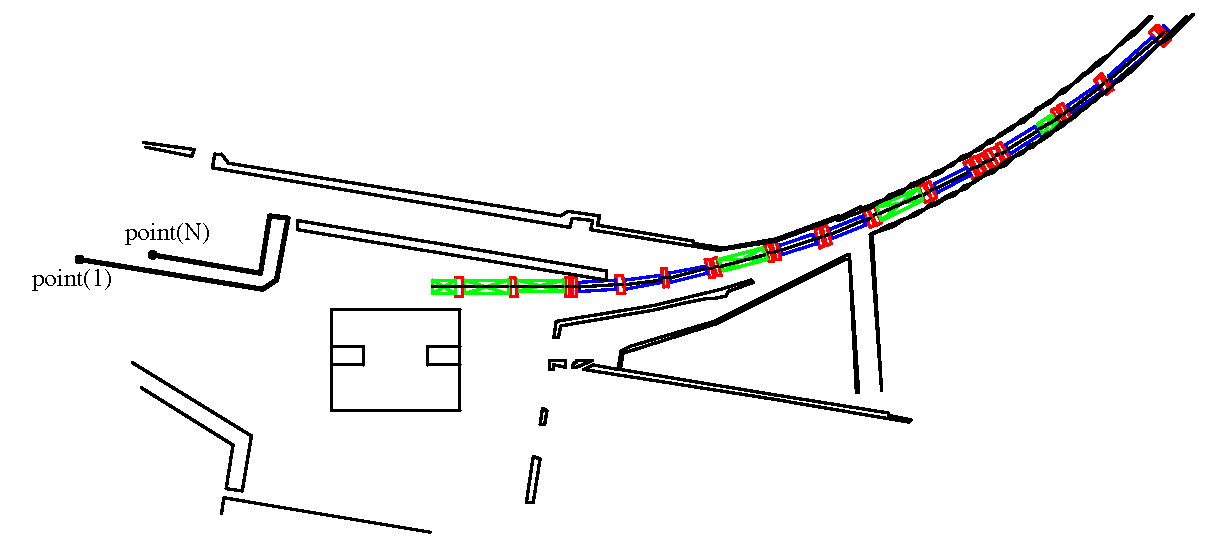
\includegraphics[width=5in]{building-wall.pdf}
  \caption[Floor_plan drawing showing the walls of the building]
{Floor_plan drawing showing the walls of the building (along with a section of a recirculation
arc). Defining building walls can be useful for such things as floor plots and designing a machine
to fit in an existing building.}
  \label{f:building.wall}
\end{figure}

A two dimensional cross-section of the building containing the machine under simulation may be defined in
\tao. This can be useful when drawing \vn{floor_plan} plots of the machine (\sref{s:floor.plan}) or
to design a machine to fit within an existing building by using optimization (\sref{c:opti}).

The wall cross-sections are defined by a set of ``\vn{sections}''. A section is a curve in the
horizontal $Z$-$X$ plane that defines where the face of a wall is. One such section is highlighted in
Figure~\ref{f:building.wall} starting at the point marked ``point(1)'' and ending at the point
marked ``point(N)''. Each section is defined by a set of points which are connected together using
straight lines or circular arcs.

The name of the file containing the building wall definition is given by the \vn{building_wall_file}
variable in the \vn{tao_start} namelist (\sref{s:init.global}). In general, this file will contain a
number of \vn{building_wall_section} namelists. Each \vn{building_wall_section} namelist defines a
single wall section. The syntax of this namelist is
\begin{example}
  &building_wall_section
    \{name = <string>\}
    \{constraint = <type>\}
    point(1) = <z1>, <x1>
    point(2) = <z2>, <x2>, \{<r2>\}
    point(3) = <z3>, <x3>, \{<r3>\}
    ... etc ...
    point(N) = <zN>, <xN>, \{<rN>\}
  /
\end{example}
The optional \vn{name} component allows for matching wall sections to \vn{floor_plan} shapes
(\sref{s:shapes}) when drawing a \vn{floor_plan} so that different portions of the wall can be drawn
in different colors.

The global coordinate system in \bmad (see the \bmad manual) defines the $(Z, X)$ plane as being
horizontal.  [Note: $(Z, X)$ is used instead of $(X, Z)$ since $(Z, X, Y)$ forms a right handed
coordinate system.] The points that define a wall section are specified in this coordinate system.
In the \vn{building_wall_section} namelist, the $(Z, X)$ position of each point defining a wall
section is given along with an optional radius $r$. If a non-zero radius is given for point $j$,
then the segment between point $j-1$ and $j$ is a circular arc of the given radius. If no radius is
given, or if it is zero, the segment is a straight line. A radius for the first point, number 1,
cannot be specified since this does not make sense. Additionally, a radius must be at least half the
distance between the two points that define the end points of the arc.

In general, given two end points and a radius, there are four possible arcs that can be drawn. The
arc chosen follows the following convention:
\begin{enumerate}
\item
The angle subtended by the arc is 180 degrees or less.
\item
If the radius for the arc from $j-1$ to $j$ is positive, the arc curves in a clockwise manner. If
the radius is negative, the arc curves counterclockwise. This convention mimics the convention used
for \vn{rbend} and \vn{sbend} elements.
\end{enumerate}
To define a wall that is circular, use three points with two 180
degree arcs in between.

When designing a machine to fit within the walls of a building, the \vn{constraint} variable of the
namelist is used to designate whether the given wall section is on the $+x$ (left) side of the
machine or the $-x$ (right) side. Here $x$ is the local reference frame transverse coordinate. See
the write up of the \vn{wall.right_side} and \vn{wall.left_side} constraints in \sref{s:data.types}
for more details. Possible values for \vn{constraint} are:
\begin{example}
  "right_side"  ! Section is to be used with wall.right_side constraints
  "left_side"   ! Section is to be used with wall.left_side constraints
  "none"        ! Default. Section is ignored in any constraint calculation.
\end{example}
Using \vn{"none"} for \vn{constraint} is convenient for drawing building components on a
\vn{floor_plan} that are not used as an optimization constraint.

Example:
\begin{example}
  &building_wall_section
    constraint = "left_side"   
    point(1) =  23.2837,    8.2842
    point(2) = -10.9703,   13.8712,   107.345
    point(3) = -10.8229,   14.7737
  /
\end{example}
In this example, point 1 is at $(Z, X) = (23.2837, 8.2842)$, the segment between points 1 and 2 is
an arc with a radius of 107.345 meters, and the segment between points 2 and 3 is a straight
line. Also this wall section is to be used when evaluating any \vn{wall.x+} constraint.

If the machine varies vertically ($y$-direction), vertical constraints may be imposed using the
\vn{floor.y} data type (\sref{s:data.types}).

To see a list of the building wall points when running \tao, use the \vn{show building_wall}
(\sref{s:show.building}) command .

Note: To position a machine in the global coordinate system, the starting point and starting
orientation can be adjusted using \vn{beginning[...]} statements as explained in the \bmad manual.

%-----------------------------------------------------------------
\subsection{Building Orientation}
\label{s:building.orient}

It may be convenient to use a different two-dimensional coordinate system for the horizontal plane
than the global coordinate system used by \bmad and \tao. For example, if the building wall coordinates are
obtained from a blueprint. To help with this, an overall position and angle
shift may be specified by a \vn{building_wall_orientation} namelist in the same file with the
\vn{building_wall_section} namelists. The syntax of the \vn{building_wall_orientation} namelist is:
\begin{example}
  theta = <Real>      ! Angle rotation in radians. Default is 0.
  z_offset = <Real>   ! Z-offset. Default is 0.
  x_offset = <Real>   ! X-offset. Default is 0.
\end{example}
The transformation from the input coordinates of a wall point specified in a \vn{build_wall_section} namelist
to the global coordinate system is
\begin{equation}
  \begin{pmatrix} z \\ x \end{pmatrix}_{global} = 
  \begin{pmatrix} \text{z_offset} \\ \text{x_offset} \end{pmatrix} +
  \begin{pmatrix} \cos(\text{theta}) & -\sin(\text{theta}) \\
                   \sin(\text{theta}) & \cos(\text{theta}) \end{pmatrix} \,
  \begin{pmatrix} z \\ x \end{pmatrix}_{input} 
\end{equation}

%-----------------------------------------------------------------
\section{Dynamic Aperture Calculation Initialization}
\index{dynamic aperture}
\label{s:da.calc}

\begin{figure}
  \centering
  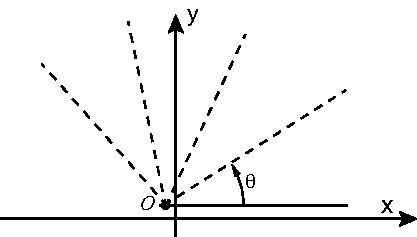
\includegraphics[width=5in]{dynamic-aperture-rays.pdf}
  \caption{
The calculation of a dynamic aperture curve in the $x$-$y$ plane at a given initial $p_z$ value
involves calculating aperture curve points (blue dots) along a set of ``rays'' (dashed lines) having
a common origin point ($\cal O$) which is taken to be the reference orbit. The line segments between
points is simply for visualization purposes. The calculation of an aperture curve point along a
given ray involves iteratively tracking particles with different starting $(x, y)$ position values
to find the boundary between stable (green dots) and unstable (red dots) motion.
  }
  \label{f:da-rays}
\end{figure}

In a storage ring, the ``\vn{dynamic aperture}'' is the region in phase space within which a
particle will stably oscillate. That is, the region within which the motion is bounded. This is in
contrast to the ``\vn{physical aperture}'' which is defined by the vacuum chamber walls. Since it
may take many turns for particle motion to become unstable, calculating the stability region for the
full six-dimensional phase space is a time intensive process.  In light of this, \tao uses a
simplified calculation as discussed below.

In \tao, the motion of a particle is taken to be ``stable'' if the particle survives (does not hit
the physical aperture or does not diverge to large amplitude) in tracking over some set number of
turns.\footnote
  {
If the dynamic aperture is larger than the physical aperture the calculated boundary curve will
reflect the physical aperture and not the dynamic aperture. In practice, this possible confusion is
not a concern since if the dynamic aperture is outside the physical aperture there is no worry that
the dynamic aperture will limit machine performance.
  }
 A typical number is 1000 turns. A dynamic aperture ``scan'' is the calculation of the dynamic
aperture in $(x, y)$ space at some given initial phase space $p_z$ as illustrated in
\fig{f:da-plot}. An $(x, y)$ point represents the initial $x$ and $y$ phase space position of
the particle with the initial $p_x$, $p_y$, and $z$ values being set equal to the closed orbit
values. To calculate an aperture curve for a given initial $p_z$, a set of ``rays" (dashed lines in
the figure) are constructed. The rays have a common origin point ($\cal O$) which is the closed
orbit $(x, y)$ point. On each ray, the boundary point between stable and unstable motion (blue
points in the figure) is found by iteratively tracking particles with initial $(x, y)$ points on the
ray (red and green dots) until the boundary point is determined with the specified accuracy.

The origin point of the rays is taken to be the closed orbit at the given $p_z$ and RF off. This is
true even if the RF is on for the tracking. The reason for this is that with the RF on, there is no
well defined closed orbit at constant $p_z$ (since $p_z$ is not a constant of the motion with the RF
on).

Having the RF off when tracking suppresses synchrotron oscillation effects which may be
important. It is therefore recommended to have the RF on unless there is a good reason for ignoring
synchrotron oscillations. It is also recommended that the lattice element at which the tracking
begins be in a zero dispersion region.

To calculate the dynamic aperture for the $i$\Th universe, the \vn{design(N)%dynamic_aperture_calc}
parameter must be set True in the \vn{tao_design_lattice} namelist (\sref{s:init.lat}). Example:
\begin{example}
  &tao_design_lattice
    design_lattice(1)%file = "lat.bmad"
    design_lattice(1)%dynamic_aperture_calc = T
  /
\end{example}
Alternatively, the aperture calculation can be turned on during running using the \vn{set} command
(\sref{s:set.universe}):
\begin{example}
  set universe 1 dynamic_aperture_calc on
\end{example}
Since aperture calculations take time, once an aperture calculation is done, the calculation is
turned off so to perform multiple scans within a given session, the \vn{set universe} command must
be repeatedly done.

The \vn{show dynamic_aperture} command (\sref{s:show.da}) shows parameter values and the
\vn{set dynamic_aperture} command (\sref{s:set.da}) can be used to change parameter values.

If Tao is compiled with \vn{OpenMP} enabled (\sref{s:openmp}), the dynamic aperture calculation will
be done in parallel.

Parameters for the dynamic aperture simulation are set in the \vn{tao_dynamic_aperture} namelist
(\sref{s:init.global}) in the \tao root initialization file. Multiple \vn{tao_dynamic_aperture}
namelists may be present if different universes need different parameter values. Example:
\begin{example}
  &tao_dynamic_aperture
    ix_universe = -1             ! Universe to apply to. -1 = all universes.
    pz = 0, 0.01, 0.15           ! List of phase space pz to start scans at.
    a_emit = 1e-11               ! A-mode emittance. Used for data calc.
    b_emit = 1e-13               ! B-mode emittance. Used for data calc.
    ellipse_scale = 10           ! Scale for drawing the ellipse in beam sigmas.
    da_param%start_ele = ''      ! Lattice element to start tracking at.
    da_param%n_angle = 21        ! Number of angles in scan of each energy
    da_param%min_angle = 0       ! Starting scan angle (rad).
    da_param%max_angle = 3.1416  ! Ending scan angle (rad).
    da_param%n_turn = 2000       ! Number of turns a particle must survive
    da_param%rel_accuracy = 1e-2 ! Relative accuracy of boundary point.
    da_param%abs_accuracy = 1e-5 ! Absolute accuracy of boundary point (meters).
    da_param%x_init = 1e-3       ! Initial horizontal aperture estimate. Default: 1e-3 meters.
    da_param%y_init = 1e-3       ! Initial vertical aperture estimate. Default: 1e-3 meters.
  /
\end{example}
Parameters:
\begin{description}
\item[ellipse_scale] \Newline
Scale for drawing the beam ellipse. The default value is 10 which will result in an ellipse drawn
at 10 sigma.
%
\item[ix_universe] \Newline
The \vn{ix_universe} parameter set which universe the parameters are applied to. Any universe index
below a value of one results in the parameter values being applied to all universes.
%
\item[pz] \Newline
The \vn{pz} parameter array is a list of $p_z$ values to use. The number of scans (dynamic aperture curves)
that are produced is equal to the number of \vn{pz} values.
%
\item[a_emit, b_emit] \Newline
Emittance values for the $a$ (``horizontal like'') and $b$ (``vertical like'') normal modes. The
emittance values do not affect particle tracking but are used to draw the beam sigma ellipse in
dynamic aperture plots (\sref{s:da.plot}) and to calculate the \vn{dynamic_aperture.$N$} datum values
(\sref{s:data.types}). 
%
\item[da_param\%start_ele] \Newline
This parameter sets the starting element for tracking. If not set, the beginning element of the
root branch is used. \vn{da_param%start_ele} may be set to either the element name or element index.
%
\item[da_param\%n_angle] \Newline
The number of boundary points calculated for a scan is set by the \vn{da_param%n_angle} parameter. 
%
\item[da_param\%min_angle, da_param\%max_angle] \Newline
These parameters set the ray minimum and maximum angles, labeled $\theta$ in \fig{f:da-plot}, in a
scan. In the example above the angle ranges from 0 to $pi$.  That is, the upper half-plane. These
are typical settings since typically storage rings are vertically symmetric so the aperture curves
should vertically symmetric as well.

The angles between adjacent rays is not uniform but are rather calculated to give a roughly
equal spacing between boundary points. This is done by looking at the aperture
points on a horizontal and a vertical ray and then scaling the ray angles appropriately).

%
\item[da_param\%rel_accuracy, da_param\%abs_accuracy] \Newline
These parameters set the relative and absolute accuracies that determine when the search for a
boundary point is considered accurate enough.

If $r = \sqrt{(x-x_0)^2 + (y-y_0)^2}$ is the distance
along any ray of the computed boundary point, where $(x_0, y_0)$ are the coordinates of the origin
point, the search for the boundary point will stop then the accuracy of the boundary point is below
the desired accuracy $\sigma_{cut}$ which is computed from
\begin{equation}
  \sigma_{cut} = \sigma_a + r \, \sigma_r
\end{equation}
with $\sigma_a$ begin the absolute accuracy and $\sigma_r$ being the relative accuracy.
%
\item[da_param\%x_init, da_param\%y_init] \Newline
These parameters set the initial $x$ and $y$ values used in the first two boundary point searches.
The values of these parameters will not affect significantly affect the computed curve but will
affect the computation time. If not set, these parameters will default to 0.001 meter.
\end{description}

To plot the results, an appropriate plot must be defined (\sref{s:da.plot}) and \vn{placed} in the
plotting window (\sref{s:init.plot}). An example dynamic aperture plot is shown in
Fig.~\ref{f:da-plot}.

Example input files for calculating and plotting the dynamic aperture are at (\sref{s:examples}):
\begin{example}
  \$ACC_ROOT_DIR/tao/examples/dynamic_aperture
\end{example}

%-----------------------------------------------------------------
\section{Initializing Plotting}
\index{plotting initializing}
\label{s:init.plot} 

\tao has a graphical display window, called the \vn{plot page} (\sref{s:plot.page.def}) within which
such things as lattice functions, machine layout, beam positions, etc., can be plotted. An example
display is shown in \fig{f:plot.typ}.

Plotting is defined by an initialization file whose name is defined by the \vn{plot_file} component
of the \vn{tao_start} namelist (\sref{s:init.global}).

%-----------------------------------------------------------------
\subsection{Plot Page and Plot Regions}
\label{s:plot.page}
\index{initialization!plotting!plot window}

The \vn{tao_plot_page} namelist (\sref{s:format}) in the plot initialization file
(\sref{s:init.global}) sets \vn{plot page} (\sref{s:plot.page.def}) parameters including \vn{region}
definitions and the initial placement of plots. The syntax of this namelist is:
\index{tao_plot_page}\index{plot_page!n_curve_pts}
\index{plot_page!size}\index{plot_page!border}
\index{plot_page!text_height}\index{plot_page!title}
\index{region!name}\index{region!location}\index{place}
\begin{example}
  &tao_plot_page
    plot_page%title                    = "<string>", <x>, <y>, "<units>", "<justify>"
    plot_page%subtitle                 = "<string>", <x>, <y>, "<units>", "<justify>"
    plot_page%plot_display_type        = "<string>"  ! Display type: "X" or "TK"
    plot_page%size                     = <x_size>, <y_size>  ! size in POINTS 
    plot_page%border                   = <qp_rect_struct>    ! Border around edge
    plot_page%text_height              = <real>   ! height in POINTS. Def = 12
    plot_page%main_title_text_scale    = <real>   ! Rel to text_height. Def = 1.3
    plot_page%graph_title_text_scale   = <real>   ! Rel to text_height. Def = 1.1
    plot_page%axis_number_text_scale   = <real>   ! Rel to text_height. Def = 0.9
    plot_page%axis_label_text_scale    = <real>   ! Rel to text_height. Def = 1.0
    plot_page%legend_text_scale        = <real>   ! Rel to text_height. Def = 0.8
    plot_page%key_table_text_scale     = <real>   ! Rel to text_height. Def = 0.9
    plot_page%floor_plan_shape_scale   = <real>   ! Floor_plan shape size scaling.
    plot_page%lat_layout_shape_scale   = <real>   ! Lat_layout shape size scaling.
    plot_page%n_curve_pts              = <int>    ! Num points used to construct a 
                                                  !   smooth curve. Default = 401
    plot_page%box_plots                = <T/F>    ! For debugging. Default = F.
    plot_page%delete_overlapping_plots = <T/F>    ! Default = T.
    plot_page%draw_graph_title_suffix  = <T/F>    ! Default = T.
    include_default_plots              = <T/F>    ! Include default templates? Def = T.
    region(N) = "<region_name>" <x1>, <x2>, <y1>, <y2>  
    place(N)  = "<region_name>", "<template_name>"
    default_plot%...                            ! See below.
    default_graph%...                           ! See below. 
  /
\end{example}

For example:
\begin{example}
  &tao_plot_page
    plot_page%title = "CESR Lattice", 0.5, 0.996, "%PAGE", "CC"
    plot_page%plot_display_type = "X"        ! X11 window.  "TK" is alternative.
    plot_page%size        = 700, 800         ! Points
    plot_page%border      = 0, 0, 0, 50, "POINTS"  
    plot_page%text_height = 12.0
    region(1) = "top"    0.0, 1.0, 0.5, 1.0
    region(2) = "bottom" 0.0, 1.0, 0.0, 0.5
    place(1)  = "top",    "orbit"
    place(2)  = "bottom", "phase"
    default_graph%x%min = 100
    default_graph%x%max = 200
  /
\end{example}

The \vn{tao_plot_page} namelist has the following parameters:
\begin{description}
%
\item[default_graph] \Newline
The \vn{default_graph} parameter is used to set defaults for any \vn{graph} component
defined in any \vn{tao_template_graph} namelist (\sref{s:template}). Example
\begin{example}
  &tao_plot_page
    default_graph%x%min = 0
    default_graph%x%max = 100
    ...
\end{example}
This sets the default \vn{x}-axis bounds. Also see \vn{default_plot} below.
%
\item[default_plot] \Newline
The \vn{default_plot} parameter is used to set defaults for any \vn{plot} component
defined in any \vn{tao_template_plot} namelist (\sref{s:template}). Example:
\begin{example}
  &tao_plot_page
    default_plot%x_axis_type = "index"
    ...
\end{example}
This sets the default \vn{%x_axis_type}. Also see \vn{default_graph} above.
%
\item[include_default_plots] \Newline
If \vn{include_default_plots} is set to \vn{False}, the collection of template plots
(\sref{s:template}) that \tao constructs by default are not constructed. The default is True.  Note:
If \vn{include_default_plots} is True, and if a user defines a template plot that has the same name
as a default plot, the default plot will not be instantiated.
%
\item[place(N)] \Newline
The \vn{place(N)} parameter, with \vn{N} being an integer, determines the initial placement of
plots (\sref{s:plot.def}).  If no \vn{place} parameters are set, the default \vn{orbit}, \vn{beta},
\vn{dispersion}, and \vn{lat_layout} plots will be displayed. Each \vn{place(N)} has the syntax:
\begin{example}
  &tao_plot_page
    place(N) = "<region_name>" "<plot_template_name>"
    ...
\end{example}
\vn{"<region_name>"} is the region name and \vn{"<plot_template_name>"} is the name of the template
plot to put in the region. Examples:
\begin{example}
  &tao_plot_page
    place(1)  = "top",    "orbit"   ! Orbit plot placed in "top" region
    place(2)  = "bottom", "phase"   ! Phase plot placed in "bottom" region
    ...
\end{example}
%
\item[plot_page\%axis_number_text_scale] \Newline
This along with \vn{plot_page%text_height} sets the font size for the plot page title. See
\vn{plot_page%text_height} for more details.
%
\item[plot_page\%axis_label_text_scale] \Newline
This along with \vn{plot_page%text_height} sets the font size for the plot page title. See
\vn{plot_page%text_height} for more details.
%
\item[plot_page\%border] \Newline
\vn{plot_page%border} sets a border around the edges of the window. As shown in
Figure~\ref{f:plot.page}, the offsets \vn{x1}, \vn{x2} in black (corresponding to \vn{%border%x1}
and \vn{%border%x2}) are the right and left border widths and the offsets \vn{y1} and \vn{y2} in
black (corresponding to \vn{%border%y1} and \vn{%border%y2}) are the bottom and top border widths
respectively. The rectangle within this border is called the \vn{plot area}.
%
\item[plot_page\%curve_legend_line_len] \Newline
Sets the length, in points, of lines drawn for the curve legend (\sref{s:plot.def}). Default is 30.
%
\item[plot_page\%curve_legend_text_offset] \Newline
Sets the space, in points, between the line and text in the curve legend. Default is 6.
%
\item[plot_page\%delete_overlapping_plots] \Newline
When \vn{plot_page%delete_overlapping_plots} is True (the default), Placing a plot (using
the \vn{place} command \sref{s:place}) causes any existing plots that overlap the
placed plot to become invisible. 
%
\item[plot_page\%draw_graph_title_suffix] \Newline
The \vn{plot_page%draw_graph_title_suffix} is used to suppress the drawing of the string that
is printed to the right of a graph title (set by \vn{graph%title}). This string is set by \tao
and has information on what is being plotted (typically the \vn{curve%component}). To suppress
the suffix, set \vn{plot_page%draw_graph_title_suffix} to False.
%
\item[plot_page\%floor_plan_shape_scale] \Newline
This parameter sets the overall scale for drawing shapes for a \vn{floor_plan} drawing
(\sref{s:shapes}). The default value is 1.
%
\item[plot_page\%graph_title_text_scale] \Newline
This along with \vn{plot_page%text_height} sets the font size for the plot page title. See
\vn{plot_page%text_height} for more details.
%
\item[plot_page\%key_table_text_scale] \Newline
This along with \vn{plot_page%text_height} sets the font size for the plot page title. See
\vn{plot_page%text_height} for more details.
%
\item[plot_page\%lat_layout_shape_scale] \Newline
This parameter sets the overall scale for drawing shapes for a \vn{lat_layout} drawing
(\sref{s:shapes}). The default value is 1.
%
\item[plot_page\%legend_text_scale] \Newline
This along with \vn{plot_page%text_height} sets the font size for the plot page title. See
\vn{plot_page%text_height} for more details.
%
\item[plot_page\%main_title_text_scale] \Newline
This along with \vn{plot_page%text_height} sets the font size for the plot page title. See
\vn{plot_page%text_height} for more details.
%
\item[plot_page\%n_curve_pts] \Newline
The \vn{plot_page%n_curve_pts} parameter sets the default number of points to use for drawing
``smooth'' curves. The default is 401. This default may be overridden for individual plots by
setting the \vn{plot%n_curve_pts} component of a plot (\sref{s:template}). If \vn{plot%n_curve_pts}
is set for an individual plot, that value overrides the value of
\vn{plot_page%n_curve_pts}. Warning: \tao will cache intermediate calculations used to compute a
smooth curve to use in the computation of other smooth curves. \tao will only do this for curves
that have \vn{plot_page%n_curve_pts} number of points. Depending upon the circumstances, setting
\vn{plot%n_curve_pts} for individual plots may slow down plotting calculations significantly.
%
\item[plot_page\%plot_display_type] \Newline
The \vn{plot_page%plot_display_type} component sets the type of plot display
window used. possibilities are:
\begin{example}
  "X"      X11 window
  "TK"     tk window
  "QT"     Available only when using PLPLOT (and not the default PGPLOT)
\end{example}
Note: The environmental variable \vn{ACC_PLOT_DISPLAY_TYPE} sets the default display type. You can
set this variable in your login file to avoid having to setup a \tao init file to set this.
%
\item[plot_page\%size] \Newline
The \vn{plot_page%size} parameter sets the horizontal and vertical size of the plot window in
\vn{points} (\sref{s:qp.units}).
%
\item[plot_page\%subtitle] \Newline
Subtitle text of the plot. See the description for \vn{plot_page%title}. The defaults here are the
same as \vn{plot_page%title} except that \vn{y} defaults to 0.97.
%
\item[plot_page\%text_height] \Newline
The \vn{plot_page%text_height} parameter sets the overall height of the text that is
drawn. Relative to this, various parameters can be used to scale
individual types of text:
\begin{example}
  &tao_plot_page
    plot_page%main_title_text_scale  = 1.3 ! Main title height. 
    plot_page%graph_title_text_scale = 1.1 ! Graph title height.
    plot_page%axis_number_text_scale = 0.9 ! Axis number height
    plot_page%axis_label_text_scale  = 1.0 ! Axis label height.
    plot_page%key_table_text_scale   = 0.8 ! Key Table text (\sref{s:key.table}).
    plot_page%legend_text_scale      = 0.9 ! Lat Layout or floor plan text.
    ...
\end{example}
The default values for these scales are given above.
%
\item[plot_page\%title] \Newline
The \vn{plot_page%title} sets the page title which is text that is generally printed at the top of
the page.  This parameter is a structure which has components:
\begin{example}
  string = ""         ! Text to print
  x = 0.50            ! Horizontal position
  y = 0.99            ! Vertical position
  units = "%PAGE"     ! Units of x and y (\sref{s:qp.units})
  justify = "CC"      ! Justification (\sref{s:qp.str.just})
\end{example}
The values shown are the defaults.
Also see \vn{page%subtitle}.
%
\item[region(N)] \Newline
The \vn{region(N)} parameter, with \vn{N} being an integer, is used to create custom regions
(\sref{s:region.def}) in addition to the default regions defined by \tao. 
Each \vn{region(N)} has the syntax:
\begin{example}
    region(N) = "<region_name>" <x1>, <x2>, <y1>, <y2>  
\end{example}
\vn{"<region_name>"} is the region name which may not contain a dot ``.'' or a space.  The other
four elements \vn{<x1>}, \vn{<x2>}, \vn{<y1>}, and \vn{<y2>} define the region position on the plot
page as discussed in \Sref{s:region.def}. There is no upper limit to the number of regions that can
be defined.
\begin{example}
  &tao_plot_page
    region(1) = "top"    0.0, 1.0, 0.5, 1.0
    region(2) = "bottom" 0.0, 1.0, 0.0, 0.5
    ...
\end{example}
%
\end{description}

%-----------------------------------------------------------------
\subsection{Plot Templates}
\label{s:template}
\index{plot templates}

A plot \vn{template} (\sref{s:plot.def}) defines a set of parameters used for constructing a
\vn{displayed} plot. \tao, by default, defines a number of template plots. User defined template
plots are constructed with a \vn{tao_template_plot} namelist in the plot initialization file
(\sref{s:init.global}) along with zero or more \vn{tao_template_graph} namelists, one for each
\vn{graph} associated with the template plot. The syntax for the \vn{tao_template_plot} is:
\index{tao_template_plot}
\index{plot!name}
\index{plot!x}
\index{plot!x_axis_type}
\index{plot!n_graph}
\index{plot!autoscale_gang_x}
\index{plot!autoscale_gang_y}
\index{plot!autoscale_x}
\index{plot!autoscale_y}
\begin{example}
  &tao_template_plot
    plot%name        = "<plot_name>"
    plot%x_axis_type = "<x_axis_type>"   ! "index", "ele_index" "s", "lat", "var", etc. 
    plot%autoscale_gang_x = <logical>    ! Default: True.
    plot%autoscale_gang_y = <logical>    ! Default: True.
    plot%autoscale_x = <logical>         ! Default: False.
    plot%autoscale_y = <logical>         ! Default: False.
    plot%n_curve_pts = <integer>         ! Used to override plot_page%n_curve_pts.
    plot%n_graph     = <n_graphs>
    default_graph%...                    ! See below
    default_curve%...                    ! See below
  /
\end{example}
For example:
\begin{example}
  &tao_template_plot
    plot%name                         = "orbit"
    default_graph%x%major_div_nominal = 10
    default_graph%x%label             = "Index"
    default_graph%y%max               = 10
    plot%n_graph                      = 2
  /
\end{example}

The \vn{tao_plot_page} namelist has the following parameters:
\begin{description}
%
\item[default_curve] \Newline
The \vn{default_curve} sets defaults for \vn{curves} associated with the plot. 
The \vn{default_curve} is a structure with the same components
as the \vn{curve} parameter of the \vn{tao_template_graph} structure discussed below.
%
\item[default_graph] \Newline
The \vn{default_graph} sets defaults for \vn{graphs} associated with the plot. This is useful if
there are multiple associated graphs. The \vn{default_graph} is a structure with the same components
as the \vn{graph} parameter of the \vn{tao_template_graph} structure discussed below.

Settings of \vn{default_graph} in the \vn{tao_template_plot} namelist overrides, for the graphs
associated with the plot, any \vn{default_graph} settings made in the \vn{tao_template_plot}
namelist (\sref{s:init.plot}).
%
\item[plot\%autoscale_gang_x] \Newline
The \vn{plot%autoscale_gang_x} parameter is relavent if the plot has more than one associated
graph. In this case, if set to True (the default), and if the \vn{x_scale} command
(\sref{s:x.scale}) is applied to the plot (as opposed to being applied to an individual graph),
the data of all the graphs is combined to compute a horizontal scale which is used for all the graphs.
If \vn{%autoscale_gang_x} is set to False, graphs are scaled individually.
%
\item[plot\%autoscale_gang_y] \Newline
The \vn{plot%autoscale_gang_y} parameter is relavent if the plot has more than one associated
graph. In this case, if set to True (the default), and if the \vn{scale} command
(\sref{s:scale}) is applied to the plot (as opposed to being applied to an individual graph),
the data of all the graphs is combined to compute a vertical scale which is used for all the graphs.
If \vn{%autoscale_gang_y} is set to False, graphs are scaled individually.
%
\item[plot\%autoscale_x] \Newline
Plots with \vn{plot%autoscale_x} set to True will
automatically rescale the horizontal axis after any calculation. Default is False.
%
\item[plot\%autoscale_y] \Newline
Plots with \vn{plot%autoscale_y} set to True will
automatically rescale the vertical axes after any calculation. Default is False.
%
\item[plot\%n_curve_pts] \Newline
The \vn{plot%n_curve_pts} parameter sets the number of evaluation points to use for drawing
``smooth'' curves (\sref{s:curve.def}). This overrides the setting of \vn{plot_page%n_curve_pts}
(\sref{s:init.plot}). Warning: \tao will cache intermediate calculations used to compute a smooth
curve to use in the computation of other smooth curves. \tao will only do this for curves that have
\vn{plot_page%n_curve_pts} number of points. Depending upon the circumstances, setting
\vn{plot%n_curve_pts} for individual plots may slow down plotting calculations significantly.
%
\item[plot\%n_graph] \Newline
The \vn{plot%n_graph} parameter sets the number of graphs associated with the plot and each one
needs a \vn{tao_template_graph} namelist to define it. These namelists should be placed directly
after their respective \vn{tao_template_graph} namelist.
%
\item[plot\%name] \Newline
The \vn{plot%name} parameter is the name that is used with \tao commands to identify the plot
(\sref{s:plot.def}). It is important that this name not contain any blank spaces since \tao uses
this fact in parsing the command line.
%
\item[plot\%x_axis_type] \Newline
The \vn{plot%x_axis_type} parameter sets what is plotted along the \vn{x_axis}. Possibilities are:
\index{index}\index{ele_index}\index{s}
\begin{example}
    "index"         ! Data Index.
    "ele_index"     ! Element lattice number index.
    "s"             ! Longitudinal position in the lattice.
    "s_expression"  ! s-dependent expression involving lattice parameters.
    "data"          ! From a data array.
    "lat"           ! Lattice variable. See \sref{s:plot.var}.
    "var"           ! Tao variable value. See \sref{s:plot.var}.
    "phase_space"   ! Set by \tao if graph%type = "phase_space".
    "none"          ! Set by \tao if graph%type = "key_table".
    "floor"         ! Set by \tao if graph%type = "floor_plan".
\end{example}

The \vn{ele_index} switch is used when plotting data arrays. In this
case the \vn{index} switch refers to the index of the data array and
\vn{ele_index} refers to the index of the lattice element that the
datum was evaluated at.
%
\end{description}

The number of graphs associated with a template plot is specified by the setting of
\vn{plot%n_graph} in the \vn{tao_template_plot} namelist.  For each associated graph there needs to
be a \vn{tao_template_graph} namelist. These namelists need to be placed directly below the
\vn{tao_template_plot} namelist. Each \vn{tao_template_graph} namelist must have a \vn{graph_index}
parameter with the first \vn{tao_template_graph} namelist below the \vn{tao_template_plot} namelist
having \vn{graph_index} set to \vn{1}, the next \vn{tao_template_graph} having \vn{graph_index} set
to \vn{2}, etc.

The general format of the \vn{tao_template_graph} namelist is:
\index{tao_template_graph}\index{graph!y}\index{curve!name}
\index{graph_index}\index{graph}\index{graph!name}\index{curve}
\index{graph!type}\index{graph!box}\index{graph!title}\index{graph!margin}
\index{graph!y2}\index{graph!n_curve}\index{graph!clip}\index{graph!component}
\index{graph!symbol_size_scale}
\index{curve!data_type}\index{curve!data_source}
\index{curve!x_axis_units_factor}\index{curve!y_axis_units_factor}
\index{curve!use_y2}\index{curve!line}\index{curve!ele_ref_name}
\index{curve!draw_line}\index{curve!draw_symbols}\index{curve!ix_universe}
\index{curve!symbol}\index{curve!symbol_every}\index{curve!convert}
\index{curve!ix_bunch}\index{curve!data_type_x}
\begin{example}
  &tao_template_graph
    graph_index              = <integer>          ! Graph index. 1 = first graph, etc.
    graph%name               = "<string>"         ! Default is  "g<n>" <n> = graph_index. 
    graph%type               = "<string>"         ! "data", "floor_plan", etc.
    graph%box                = <ix>, <iy>, <ix_tot>, <iy_tot>
    graph%title              = "<string>"         ! Title above the graph.
    graph%text_legend(n)     = "<string>"         ! Set legend text
    graph%text_legend_origin  = <qp_point_struct> ! Placement of the text legend
    graph%curve_legend_origin = <qp_point_struct> ! Placement of the curve legend
    graph%margin             =  <ix1>, <ix2>, <iy1>, <iy2>, "<Units>"
    graph%scale_margin       =  <ix1>, <ix2>, <iy1>, <iy2>, "<Units>"
    graph%x                  = <qp_axis_struct>   ! Horizontal axis.
    graph%y                  = <qp_axis_struct>   ! Left axis.
    graph%y2                 = <qp_axis_struct>   ! Right axis.
    graph%y2_mirrors_y       = <logical>          ! y2 min/max the same as y-axis? Default = T
    graph%clip               = <logical>          ! Clip curves at boundary? Default = T
    graph%draw_axes          = <logical>          ! Default = T
    graph%draw_grid          = <logical>          ! Default = T
    graph%draw_curve_legend  = <logical>          ! Default = T
    graph%draw_title         = <logical>          ! Default = T
    graph%allow_wrap_around  = <logical>          ! Wrap curves around lattice ends?
    graph%symbol_size_scale  = <real>             ! Phase_space plots symbol scale factor
    graph%ix_universe        = <integer>          ! Default = -1 => Use default universe
    graph%ix_branch          = <integer>          ! Lattice branch index.
    graph%floor_plan         = <floor_plan_struct> ! Floor_plan parameters (\sref{s:floor.plan}).
    graph%draw_only_good_user_data_or_vars        ! Veto data or variables with good_user = F?
                                 = <logical>      !   Default = T.
    graph%x_axis_scale_factor    = <factor>       ! Scale the x-axis by this.
    graph%n_curve                = <integer>      ! Limit number of curves.
    curve(N)%name                = "<string>"     ! Default is "c<i>", <i> = curve num.
    curve(N)%data_type           = "<string>"     ! EG: "orbit.x"
    curve(N)%data_source         = "<string>"     ! Source for the data curve points
    curve(N)%data_type_x         = "<string>"     ! Used with plot%x_axis_type = "data" or "var".
    curve(N)%component           = "<string>"     ! Eg: "model - design". 
    curve(N)%data_index          = "<string>"     ! Index number for data points.
    curve(N)%legend_text         = "<string>"     ! Text for curve legend. 
    curve(N)%y_axis_scale_factor = <factor>       ! Scale the y-axis by this.
    curve(N)%use_y2              = <logical>      ! Use left-axis scale?
    curve(N)%draw_line           = <logical>      ! Connect data with lines?
    curve(N)%draw_symbols        = <logical>      ! Draw data symbols?
    curve(N)%draw_symbol_index   = <logical>      ! Print index number next to the data symbol?
    curve(N)%draw_error_bars     = <logical>      ! Draw error bars with data?
    curve(N)%ix_universe         = <integer>      ! Default = -1 => Use graph%ix_universe.
    curve(N)%ix_branch           = <integer>      ! Default = 0  => Use main lattice.  
    curve(N)%ix_bunch            = <integer>      ! Bunch index. Default = 0 (all bunches).
    curve(N)%n_turn              = <integer>      ! For phase space multi_turn_orbit.
    curve(N)%line     = <qp_line_struct>          ! Line spec (color, width, etc.)
    curve(N)%symbol   = <qp_symbol_struct>        ! Symbol spec (color size, etc.)
    curve(N)%symbol_every      = <integer>        ! Plot symbol every # datums
    curve(N)%ele_ref_name      = "<string>"       ! Name of reference element.
    curve(N)%smooth_line_calc  = <Logical>        ! Calc data between symbol points? 
    curve(N)%orbit   = <tao_graph_orbit_struct>   ! For E & B field plots
    curve(N)%hist    = <tao_histogram_struct>     ! For histograms
    curve(N)%z_color = <tao_curve_color_struct>   ! For phase space plotting
  /
\end{example}
For example:
\begin{example}
  &tao_template_graph
    graph_index               = 1
    graph%name                = "x"
    graph%type                = "data"
    graph%box                 = 1, 1, 1, 2
    graph%title               = "Horizontal Orbit (mm)"
    graph%margin              =  60, 200, 30, 30, "POINTS"
    graph%y%label             = "X"
    graph%y%major_div_nominal = 4
    curve(1)%component        = "model - design"
    curve(1)%data_source      = "data"
    curve(1)%data_type        = "orbit.x"
    curve(1)%units_factor     = 1000
    curve(1)%use_y2           = F
  /
\end{example}

The \vn{tao_template_graph} namelist has the following parameters:
\begin{description}
%
\item[curve(N)\%component] \Newline
The \vn{%component} sets from where data is derived from (\sref{s:curve.comp}).
%
\item[curve(N)\%data_index] \Newline
When used with graphing a data slice (\sref{s:graph.data.slice}), the \vn{%data_index}
parameter sets the index number for the symbol points. The symbol index number can then be displayed
next to the symbol.

When used with graphing the dynamic aperture (\sref{s:da.plot}), the \vn{%data_index} parameter
is used to associate a curve with a given dynamic aperture scan.
%
\item[curve(N)\%data_source] \Newline
The \vn{%data_source} parameter sets where information is drawn in computing curve points
(\sref{s:curve.source}). Used in conjunction with \vn{%data_type} and \vn{%component}. 
%
\item[curve(N)\%data_type] \Newline
The \vn{%data_type} parameter sets what is being computed (\sref{s:curve.type}). Used in
conjunction with \vn{%data_type} and \vn{%component}.
%
\item[curve(N)\%data_type_x] \Newline
Used with data slices (\sref{s:graph.data.slice}).
%
\item[curve(N)\%draw_error_bars] \Newline
The \vn{%draw_error_bars} logical determines whether error bars are drawn when plotting data
(\vn{%data_source} set to \vn{data}). The half height of the error bars is determined by the
\vn{error_rms} values of the data associated with the curve (\sref{s:data.anatomy}).  To keep things
simple, \tao ignores the setting of \vn{%component} when drawing error bars. This must be kept
in mind since for example, the measurement error associated with a difference plot of measured data
minus reference data (when \vn{%component} is set to \vn{meas-ref}) is different from just plotting
measured data, which in turn is different from a plot of the data as calculated from the \vn{model}
(the measurement error associated with this is zero).
%
\item[curve(N)\%draw_line] \Newline
Used to toggle drawing of the curved line associated with a curve (\sref{s:curve.line}). Default is True.
%
\item[curve(N)\%draw_symbol_index] \Newline
Used to toggle drawing of the symbol index. Default is False.
%
\item[curve(N)\%draw_symbols] \Newline
Used to toggle drawing of symbols. Default is True.
%
\item[curve(N)\%ele_ref_name] \Newline
The \vn{%ele_ref_name} component is only used if \vn{%data_source} is set to \vn{"lat"}.
If \vn{%ele_ref_name} is set, the curve will be shifted by subtracting the value of the
parameter being plotted evaluated at the reference element. For example, if \vn{orbit.x} is being
plotted, and \vn{%ele_ref_name} is set to "\vn{Q10W}", the plotted curve will be shifted by
subtracting the value of the horizontal orbit at Q10W. Notice that the shifting is done for each
curve component. For example, if \vn{%component} is set to "\vn{model - design}", the curve
will be shifted by subtracting the difference between the \vn{model} and \vn{design} values
evaluated at the reference element.
%
\item[curve(N)\%hist] \Newline
The \vn{%hist} parameter is a structure used for setting histogram parameters (\sref{s:histogram}).
%
\item[curve(N)\%ix_branch] \Newline
The \vn{%ix_branch} sets which lattice branch data (beta function, orbit, etc.) is taken.
from. Default is branch 0 (the root branch). 
%
\item[curve(N)\%ix_bunch] \Newline
The \vn{%ix_bunch} parameter sets which particle bunch data is taken from if \vn{%data_source}
(\sref{s:curve.source}) is set to \vn{"beam"}. Default is 1.
%
\item[curve(N)\%ix_universe] \Newline
The \vn{%ix_universe} parameter sets which universe (\sref{s:universe}) data is taken from. Default
is -1 which means that the data will be drawn from the current default universe.
%
\item[curve(N)\%legend_text] \Newline
The \vn{%legend_text} parameter sets the text that is displayed in the curve legend
(\sref{s:curve.legend}) for the curve.
%
\item[curve(N)\%line] \Newline
The \vn{%line} parameter sets parameters associated with curved line associated with the curve
(\sref{s:curve.line}).  This parameter is a structure of type \vn{qp_line_struct}
(\sref{s:qp.line}).
%
\item[curve(N)\%name] \Newline
The identifying name of the curve (\sref{s:curve.name}). Used in \tao commands that manipulate curves.
%
\item[curve(N)\%orbit] \Newline
The \vn{%orbit} parameter, used when plotting electric and magnetic fields, defines the orbit with
constant transverse offset along which the fields are evaluated. This parameter is used when the
\vn{%data_type} is one of the following:
\begin{example}
  b0_field.x,  b0_field.y,  b0_field.z,  b0_curl.x,  b0_curl.y,  b0_curl.z,  b0_div
  e0_field.x,  e0_field.y,  e0_field.z,  e0_curl.x,  e0_curl.y,  e0_curl.z,  e0_div
\end{example}
Note: The data types with names starting with ``b_'' and ``e_'' evaluate the field along the single
particle trajectory.

The \vn{%orbit} is a structure with the following subcomponents:
\begin{example}
  x         ! horizontal $x$-position of orbit.
  y         ! vertical $y$-position of orbit.
  t         ! time to evaluate fields at.
\end{example}
%
\item[curve(N)\%smooth_line_calc] \Newline
Sets if additional points are used to evaluate the curve at so that the drawn line has a ``smooth''
appearance (\sref{s:curve.line}). Default is True.
%
\item[curve(N)\%symbol] \Newline
The \vn{%symbol} parameter sets parameters associated with the symbols to be drawn
(\sref{s:curve.sym}). This parameter is a structure of type \vn{qp_symbol_struct} (\sref{s:qp.sym}).
%
\item[curve(N)\%symbol_every] \Newline
When drawing a set of symbols of a curve, if the density of symbols is too large so that the drawing
is too crowded, The number can be reduced by a factor equal to the value of \vn{%symbol_every}. For
example, a setting of \vn{3} will result in every third symbol being drawn. This is especially
helpful in phase space plots. The default is \vn{1}.
%
\item[curve(N)\%use_y2] \Newline
Use the \vn{y2} axis (\sref{s:axes}) for the curve? Default is False.
%
\item[curve(N)\%y_axis_scale_factor] \Newline
Curve vertical \vn{y} and \vn{y2} axes scale factor. For a given ``datum'' value, the plotted value will be:
\begin{example}
  y(plotted) = scale_factor * y(datum)
\end{example}
The default value is \vn{1}. For example, a \vn{%y_axis_scale_factor} of 1000 will draw a 1.0~mm orbit at the
1.0 mark on the vertical scale. That is, the vertical scale will be in millimeters.
\vn{graph%x_axis_scale_factor}.
%
\item[curve(N)\%z_color] \Newline
The \vn{%z_color} parameter is a structure used for setting false color parameters for phase space
plotting. See \Sref{s:phase.space} for more details.
%
\item[graph\%allow_wrap_around] \Newline
If \vn{plot%x_axis_type} is set to \vn{"s"}, and if the plotted data is from a lattice branch with a
closed geometry, and if \vn{graph%x%min} is negative, then the \vn{graph%allow_wrap_around}
parameter sets if the curves contained in the graph are ``wrapped around'' the beginning of the
lattice so that the curves are not cut off at $s = 0$. The default is \vn{True}.
%
\item[graph\%box] \Newline
The \vn{graph%box} parameter sets the layout of the box which the \vn{graph} is placed in
\sref{s:box.def}. In the above example, the graph divides the \vn{region} the plot is placed in into
two vertically stacked rectangles and the graph will be placed into the bottom one. The default
is \vn{1,1,1,1} which scales a graph to cover the entire \vn{region} the plot is placed in.
%
\item[graph\%clip] \Newline
Clip the graph curves at the graph top and bottom boundaries? Default is \vn{True}.
%
\item[graph\%curve_legend_origin]\Newline
The curve legend displays which curves are associated with which of the plotted lines and symbols. Two
examples are given \fig{f:plot.typ}. The \vn{%curve_legend_origin} defines where the upper left hand
corner of the legend is. The default is:
\begin{example}
  graph%curve_legend_origin%x =  5.0
  graph%curve_legend_origin%y = -2.0
  graph%curve_legend_origin%units = "POINTS/GRAPH/LT"
\end{example}
The \vn{%curve_legend_origin} is of type \vn{qp_point_struct}. See \sref{s:qp.point} for details on this
structure. Also see \vn{graph%draw_curve_legend}
%
\item[graph\%draw_axes] \Newline
Draw the graph axes? Default is \vn{True}. 
%
\item[graph\%draw_curve_legend] \Newline
Draw the curve legend? Default is \vn{True}. The curve legend displays which curves are associated
with which of the plotted lines and symbols. Two examples are given \fig{f:plot.typ}. Also see
\vn{graph%curve_legend_origin}.
%
\item[graph\%draw_grid] \Newline
Draw the graph grid? Default is \vn{True}.
%
\item[graph\%draw_only_good_user_data_or_vars] \Newline
When plotting \tao data (\sref{c:data}) or variables (\sref{c:var}): If
\vn{%draw_only_good_user_data_or_vars} is set to True (the default), symbol points of curves in the
graph associated with data or variables whose \vn{good_user} parameter is set to \vn{False} will be
ignored. That is, data and variables that will not be used in an optimization will be ignored. If
\vn{%draw_only_good_user_data_or_vars} is set to False, data or variables that have a valid value
will be plotted.
%
\item[graph\%draw_title] \Newline
Draw the graph title? Default is True.
%
\item[graph\%floor_plan] \Newline
This parameter is a structure whose components are used when drawing a \vn{floor_plan}. See
\Sref{s:floor.plan} for more details.
%
\item[graph\%ix_branch] \Newline
The \vn{graph%ix_branch} parameter sets the default branch for curves of the graph. The default will
be overridden by \vn{curve(N)%ix_branch}. 
%
\item[graph\%ix_universe] \Newline
The \vn{graph%ix_universe} parameter sets the default universe for curves of the graph.
%
\item[graph\%margin] \Newline
\vn{graph%margin} sets the margin between the \vn{graph} and the \vn{box}
it is drawn in.
%
\item[graph\%n_curve] \Newline
If not present, \tao will count the number of curves associated with a graph based on if
\vn{curve(N)%data_type} is set. In the case where \vn{default_curve%data_type} in the
\vn{tao_template_plot} namelist is set, the \vn{graph%n_curve} parameter can be set to
limit the number of curves created.
%
\item[graph\%name] \Newline
\vn{graph%name} and \vn{curve%name} define names to be used with commands. The default names are
just the letter \vn{g} or \vn{c} with the index of the graph or curve. Thus, in the example above,
the name of the curve defaults to \vn{c1} and it would be referred to as \vn{orbit.x.c1}.  It is
important that these names do not contain any blank spaces since \tao uses this fact in parsing the
command line.
%
\item[graph\%scale_margin] \Newline
\vn{graph%scale_margin} is used to set the minimum space between what is being drawn and the edges
of the \vn{graph} when a \vn{scale}, \vn{x_scale}, or a \vn{xy_scale} command is issued. Normally
this is zero but is useful for \vn{floor plan} drawings.
%
\item[graph\%symbol_size_scale] \Newline
%
\item[graph\%text_legend]\Newline
%
\item[graph\%text_legend_origin]\Newline
%
\item[graph\%title] \Newline
The \vn{graph%title} component is the string printed just above the graph box. The full string will also
include information about what is being plotted and the horizontal axis type. To fully suppress the
title leave it blank. Note: A graph also has a \vn{graph%title_suffix} which \tao uses to hold the
string which is printed to the right of the \vn{graph%title}. This string contains information like
what \vn{curve%component} is being plotted. The \vn{graph%title_suffix} cannot be set by the user.
%
\item[graph\%type] \Newline
\vn{graph%type} is the type of graph. \tao knows about the
following types:
\index{data}\index{lat_layout}\index{key_table}\index{phase_space}
\index{floor_plan}\index{beam_chamber_wall}
\begin{example}
  "data"               ! Lattice parameters, data and/or variable plots (default).
  "dynamic_aperture"   ! Dynamic aperture plot (\sref{s:da.plot}).
  "floor_plan"         ! A 2-dimensional birds-eye view of the machine (\sref{s:floor.plan}).
  "histogram"          ! Histogram of plot (\sref{s:histogram}).
  "key_table"          ! Key binding table for single mode (\sref{s:key.table}).
  "lat_layout"         ! Schematic showing placement of the lattice elements (\sref{s:lat.layout}).
  "phase_space"        ! Phase space plots (\sref{s:phase.space}).
\end{example}

With \vn{graph%type} set to \vn{"data"} (\sref{s:graph.types}), data such as orbits and/or variable
values such as quadrupole strengths are plotted. Here ``data'' can be data from a defined data
structure (\sref{c:data}) or computed directly from the lattice, beam tracking, etc. A \vn{"data"}
graph type will contain a number of \vn{curves} and multiple data and variable curves can be drawn
in one graph.

With \vn{graph%type} set to \vn{floor_plan} (\sref{s:floor.plan}), the two dimensional layout of the
machine is drawn.

With \vn{graph%type} set to \vn{histogram} (\sref{s:histogram}), such things such as beam densities
can be histogrammed.

With \vn{graph%type} set to \vn{"key_table"} (\sref{s:key.table}), the key bindings for use in
single mode (\sref{s:key.bind}) are displayed.  Note: The \vn{"key_table"} graph type does not have
any associated \vn{curve}s.

With \vn{graph%type} set to \vn{lat_layout} (\sref{s:lat.layout}), the elements of the lattice are
symbolical drawn in a one dimensional line as a function of the longitudinal distance along the
machine centerline.

With \vn{graph%type} set to \vn{phase_space} (\sref{s:phase.space}), phase space plots are produced.
%
\item[graph\%x] \Newline
The \vn{%x} parameter sets parameters for the \vn{x}-axis (\sref{s:axes}). This parameter is a
structure of type \vn{qp_axis_struct}. See \Sref{s:qp.axis} for more details.
%
\item[graph\%x_axis_scale_factor] \Newline
Sets the horizontal \vn{x}-axis scale factor. For a given ``datum'' value, the plotted value will
be:
\begin{example}
  x(plotted) = scale_factor * x(datum)
\end{example}
The default value is \vn{1}. For example, a \vn{%x_axis_scale_factor} of 1000 will draw a 1.0~mm
phase space $z$ value at the 1.0 mark on the horizontal scale. That is, the horizontal scale will be
in millimeters. Also see \vn{curve(N)%y_axis_scale_factor}.
%
\item[graph\%y] \Newline
The \vn{%y} parameter sets parameters for the \vn{y}-axis (\sref{s:axes}). This parameter is a
structure of type \vn{qp_axis_struct}. See \Sref{s:qp.axis} for more details.
%
\item[graph\%y2] \Newline
The \vn{%y2} parameter sets parameters for the \vn{y2}-axis (\sref{s:axes}). This parameter is a
structure of type \vn{qp_axis_struct}. See \Sref{s:qp.axis} for more details.
%
\item[graph_index] \Newline
The first \vn{tao_template_graph} namelist after the associated \vn{tao_template_plot} namelist must
have the \vn{graph_index} component set to \vn{1}. The next must have \vn{graph_index} set to
\vn{2}, etc. \tao uses the \vn{graph_index} component to check for errors.
%
\end{description}

%-----------------------------------------------------------------
\subsection{Graphing Lattice Parameters}\index{plot!lattice functions}
\label{s:graph.lat.fun}

Templates for plotting lattice parameters such as Twiss parameters or the orbit can be defined by setting
the \vn{data_type} of a curve appropriately. Example:
\begin{example}
  &tao_template_plot
    plot%name = "my_orbit"
    plot%x_axis_type = "s"
    plot%n_graph = 1
    default_curve%y_axis_scale_factor = 1000  ! mm
  /

  &tao_template_graph
    graph_index = 1
    graph%name = "g"
    curve(1:2)%data_type = "orbit.x", "orbit.y"
  /
\end{example}
lattice parameter names correspond to data type name  as listed in \Sref{s:data.table}.

If the \vn{plot%x_axis_type} is set to \vn{"index"}, the horizontal axis will be the lattice element
index.

If the \vn{curve(N)%source} parameter is set to \vn{"beam"} (The default is \vn{"lat"}), beam
tracking must be done (\sref{s:beam.init}) to have a visible plot. Additionally, due to the way \tao
does beam tracking, \tao is only able to evaluate the plotted parameter at the boundaries between
lattice elements. This means that \tao is not able to do the ``smooth'' line calculation.

%-----------------------------------------------------------------
\subsection{Graphing a Data Slice}\index{plot!data slice}
\label{s:graph.data.slice}

Note: Data slicing is a type of parametric plotting. For parametric plotting using curve data see
section~\sref{s:param.plot}.

The standard data graph, as presented in the previous subsection, plots data from a given
\vn{d1_data} array. It is also possible to graph data that has been ``sliced'' in other ways. For
example, suppose a number of universes have been established, with each universe representing the
same machine but with different steerings powered. If in each universe an \vn{orbit} \vn{d2_data}
structure has been defined, an example of a data slice is the collection of points (x, y) where:
\begin{example}
  (x, y) = (<n>@orbit.x[23], <n>@orbit.y[23]),  <n> = 1, ..., n_universe
\end{example}
When defining a template for graphing a data slice, the \vn{plot%x_axis_type} is set to \vn{"data"}, and
the \vn{graph%type} must be set to \vn{"data"}, the \vn{curve(:)%data_source} must be set to
\vn{"data"} and the \vn{curve(:)%data_type_x} and \vn{curve%data_type} are used to define the $x$ and
$y$ axes respectively.  In the strings given by \vn{<curve%data_type_x} or \vn{<curve%data_type}, all
substrings that look like \vn{\#ref} are eliminated and the string given by \vn{curve%ele_ref_name}
is substituted in its place.  Similarly, a \vn{\#comp} string is used as a place holder for the
\vn{curve%component} Example:
\begin{example}
  &tao_template_plot
    plot%name = "at_bpm"
    plot%x_axis_type = "data"
    plot%n_graph = 1
  /

  &tao_template_graph
    graph_index = 1
    graph%title = "Orbit at BPM"
    graph%y%label = "y"
    graph%type = "data"
    graph%x_axis_scale_factor = 1000
    graph%x%label = "x"
    curve(1)%component   = "meas - ref"
    curve(1)%data_source = "data"
    curve(1)%data_type_x = "[2:57]@orbit.x[#ref]|#comp"
    curve(1)%data_type   = "[2:57]@orbit.y[#ref]|#comp"
    curve(1)%data_index  = "[2:57]@orbit.y[#ref]|ix_uni"
    curve(1)%y_axis_scale_factor = 1000
    curve(1)%ele_ref_name = "23"
    curve(1)%draw_line = F
  /
\end{example}
In this example, \vn{curve(1)%data_type_x} expands to \vn{"[2:57]@orbit.x[23]|meas-ref"}. That is,
the \vn{meas - ref} values of \vn{orbit.x[23]} from universes 2 through 57 is used for the x-axis.
Similarly, \vn{orbit.y[23]} is used for the y-axis. The \vn{set} command (\sref{s:set}) can be used
to change \vn{curve%ele_ref_name} and \vn{curve(1)%component} strings.

\vn{curve%data_index} sets the index number for the symbol points (\sref{s:template}). In the above
example, \vn{curve%data_index} is set to \vn{"[2:57]@orbit.y[\#ref]|ix_uni"}. The \vn{|ix_uni}
component will result in the symbol index number being the universe number.  Additionally, the
component \vn{|ix_d1} can be used to specify the index in the \vn{d1_data} array, and the component
\vn{|ix_ele} can be used to specify the lattice element index. Setting the symbol index number is
important when \vn{curve%draw_symbol_index} is set to True so that the symbol index is drawn with
the curve. Additionally, the command \vn{show curve -symbol} (\sref{s:show}) will print the symbol
index number along with the $(x, y)$ coordinates of the symbols.

Arithmetic expressions (\sref{s:arithmetic.exp}) may be mixed with explicit datum components in the
specification of \vn{curve(:)%data_type_x} and \vn{curve(:)%data_type}. Example:
\begin{example}
  curve(1)%data_type_x = "[#ref]@orbit.x|model"
  curve(1)%data_type   = "[#ref]@orbit.x|meas-ref"
  curve(1)%ele_ref_name = "3"
\end{example}
The plots the \vn{model} values of \vn{orbit.x} verses \vn{meas - ref} of \vn{orbit.x} for the data
in universe 3. Note: Whenever explicit components are specified, the \vn{curve%component} settings
are ignored for that expression.

%-----------------------------------------------------------------
\subsection{Parametric Plotting}
\label{s:param.plot}

With parametric plotting, both the $x$ and the $y$ values of the points on a curve are dependent
upon an independent parameter. An example could be plotting $\alpha_a(s)$ versus $\sqrt{\beta_b(s)}$ over
some range of the independent parameter $s$. One way to do parametric plotting is to use data slices
as discussed in section~\sref{s:graph.data.slice}. Another way to do parametric plotting, which is
discussed in this section, is to setup two plot curves whose $y$ values are the desired dependent
parameters ($\alpha_x(s)$ and $\beta_y(s)$ say) and then define a parametric curve which uses the
data from these curves.

The two curves from which the data is to be taken must be in the same graph. The $y$ values from the
first curve will be taken to define the $x$ coordinate of the parametric curve and the $y$ values
from the second curve will be taken to define the $y$ coordinate of the parametric curve. The plot
that holds these curves will be called the ``\vn{source}'' plot. Example:
\begin{example}
  &tao_template_plot
   plot%name = "src"
   plot%x_axis_type = "s"
   plot%n_graph = 1
  /

  &tao_template_graph
   graph_index = 1
   graph%name = "g"
   curve(1)%data_source = "lat"
   curve(1)%data_type = "alpha.a"
   curve(2)%data_source = "lat"
   curve(2)%data_type = "expression: sqrt(beta.b)"
\end{example}
This defines a source plot called \vn{src} with two curves which will be used in the parametric plot. 

The parametric plot curve references the source curves by setting the parametric curve's
\vn{data_source} parameter equal to \vn{"curve"} and the parametric curve's \vn{data_type} to the
graph in the source plot which contains the source curves. For example:
\begin{example}
  &tao_template_plot
    plot%name = "parametric"
    plot%n_graph = 1
    plot%x_axis_type = "curve"
  /

  &tao_template_graph
    graph_index = 1
    graph%name = "g1"
    curve(1)%data_source = "curve"
    curve(1)%data_type = "src.g"
  /
\end{example}
The parametric plot's \vn{x_axis_type} needs to be set to \vn{"curve"} along with the parametric
curve's \vn{data_source}.

When the parametric plot is \vn{placed} in the plot window, \tao will look for a suitable source
plot to connect with. If \tao does not find a suitable source plot, \tao will place a source plot in
an unused plot \vn{region} and set the plot to be invisible. The region name will be set to
\begin{example}
  <source-plot-name>_<parametric-plot-region>
\end{example}
where \vn{<source-plot-name>} is the name of the source plot and \vn{<parametric-plot-region>} is
the name of the region where the parametric plot has been placed. For example, if the above
parametric plot is placed in a region called ``\vn{r12}'', the name of the region where the source
plot is placed will be named ``\vn{src_r12}''. Note: The \vn{show plot} command will show if a plot
in a given region is visible. The \vn{set plot} (\sref{s:set.plot}) command can be used to toggle 
plot visibility.

%-----------------------------------------------------------------
\subsection{Plotting With a Variable Parameter on the X-Axis}
\index{plot!plotting as a function of a variable}
\label{s:plot.var}

Data can be plotted as a function of a lattice parameter by setting \vn{plot%x_axis_type} to
\vn{"lat"} (for lattice variables) or \vn{"var"} (for \tao variables) and setting
\vn{curve(:)%data_type_x} to the name of the variable. In this case, the \vn{curve(:)%data_type}
must evaluate to a single number.

Example:
\begin{example}
  &tao_template_plot
    plot%x_axis_type = "lat"
    plot%n_curve_pts = 50
    ...
  /

  &tao_template_graph
    ...
    curve(1)%data_type_x = "particle_start[x]"  ! X-axis values.
    curve(1)%data_type   = "orbit.x[10]"        ! Y-axis values.
    ...
  /
\end{example}
Here the number of curve points has been set to 50 to reduce the evaluation overhead.

Note: \tao treats the \vn{design} and \vn{base} lattices as static so that varying a variable will
not affect these lattices. Thus, constructing a plot with \vn{curve%component} set to, for example,
\vn{"model - design"} will {\em not} produce a plot that is the difference between varying a
variable in both \vn{model} and \vn{design} lattices. In the case where such a plot is desired, a
second universe needs to be established. In this case, one would set \vn{curve(:)%data_type} to
something like
\begin{example}
    curve(1)%data_type   = "1@orbit.x[10] - 2@orbit.x[10]"    
\end{example}
where the universe \#2 \vn{model} lattice would be setup to be equal to the universe \#1 \vn{design}
lattice.

%-----------------------------------------------------------------
\subsection{Drawing a Lattice Layout}
\index{lattice layout}
\label{s:lat.layout}

\begin{figure}
  \centering
  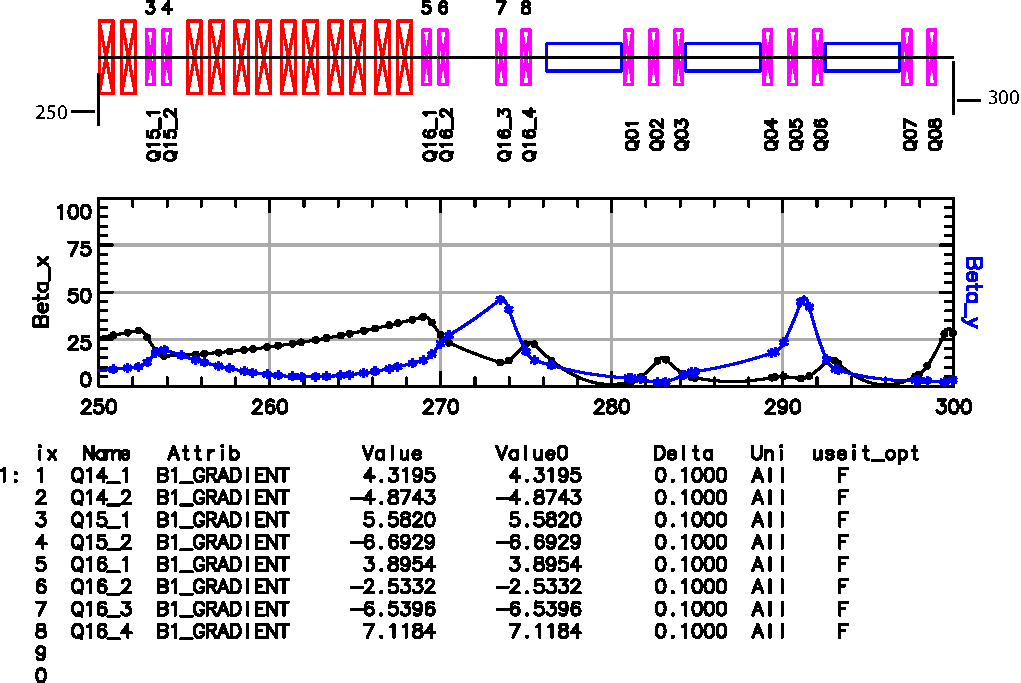
\includegraphics[width=5in]{layout-graph-table.pdf}
  \caption[Example lattice layout and data plots]
{A lattice layout plot (top) above a data plot (middle) which in turn is above a key table plot
(bottom). The points on the curves in the data plot mark the edges of the elements displayed in the
lattice layout. Elements that have attributes that are varied as shown in the key table have the
corresponding key table number printed above the element's glyph in the lattice layout.}
  \label{f:layout.table}
\end{figure}

A lattice layout plot draws the lattice along a straight line with colored rectangles representing
the various elements.  An example is shown in Figure~\ref{f:layout.table}.  The
\vn{tao_template_plot} needed to define a lattice layout looks like:
\index{tao_template_plot}\index{plot!name}
\index{plot!x!min}\index{plot!x!max}\index{plot!n_graph}
\index{tao_template_graph}\index{graph_index}\index{graph!name}
\index{graph!type}\index{graph!title}\index{graph!box}
\index{graph!ix_universe}\index{graph!margin}\index{graph!n_curve}
\begin{example}
  &tao_template_plot
    plot%name        = "<plot_name>"
    plot%n_graph     = <integer>
    plot%x_axis_type = "s"
  /
  &tao_template_graph
    graph_index       = <integer>
    graph%name        = <name>
    graph%type        = "lat_layout"
    graph%title       = "Layout Title"
    plot%box          = <ix>, <iy>, <ix_tot>, <iy_tot>
    graph%ix_universe = <integer> ! -1 => use current default universe
    graph%ix_branch   = <integer> !  0 => use main lattice.
    graph%margin      = <ix1>, <ix2>, <iy1>, <iy2>, "<Units>"
    graph%x%min       = <real>  
    graph%x%max       = <real>  
    graph%y%min       = <real>    ! Default: -100
    graph%y%max       = <real>    ! Default:  100
  /
\end{example}
Example:
\begin{example}
  &tao_template_plot
    plot%name        = "layout"
    plot%n_graph     = 1
    plot%x_axis_type = "s"
  /

  &tao_template_graph
    graph_index       = 1
    graph%name        = "u1"
    graph%type        = "lat_layout"
    graph%box         = 1, 1, 1, 1
    graph%ix_universe = -1  ! Use default universe
    graph%margin      = 0.12, 0.12, 0.30, 0.06, "%BOX"
  /
\end{example}

Which elements are drawn is under user control and is defined using an \vn{lat_layout_drawing}
namelist. See Section~\sref{s:shapes} for more details.

Setting \vn{graph%ix_universe} to -1 means the current default universe will be drawn. Normally, if
there are element shapes that are associated with data or variable shapes (\sref{s:shapes}), these
shapes will be drawn if there are lattice elements associated with the data or variables that live
in the universe with index \vn{graph%ix_universe} and if the associated elements fall within the
range of elements plotted. The exception is that if \vn{graph%ix_universe} is set to -2, the universe
of the associated lattice elements is ignored. Using a value of -2 here only makes sense if the design
lattices of all the universes is the same.

The longitudinal distance markers at either end of the lattice layout can be suppressed by setting
\begin{example}
  graph%x%draw_numbers = F
\end{example}

%-----------------------------------------------------------------
\subsection{Drawing a Floor Plan}
\index{floor plan drawing}
\label{s:floor.plan}

\begin{figure}[b]
  \centering
  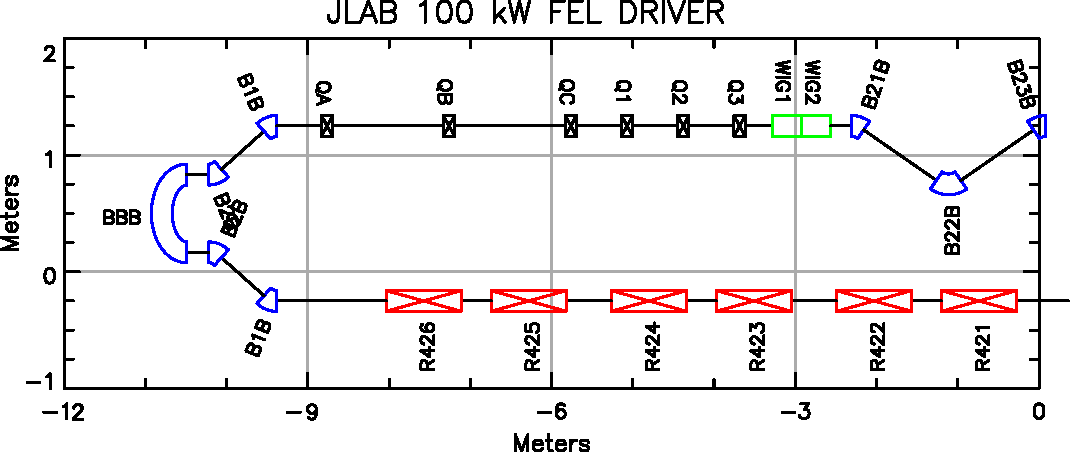
\includegraphics[width=5in]{floor-plan.pdf}
  \caption{Example Floor Plan drawing.}
  \label{f:floor.plan}
\end{figure}

A \vn{floor plan} drawing gives a display of the machine projected onto the horizontal plane.  An
example is shown in Figure~\ref{f:floor.plan}. Like a \vn{Lattice Layout} (\sref{s:lat.layout}),
Elements are represented by colored rectangles and which elements are drawn is determined by a
\vn{floor_plan_drawing} namelist (see~\sref{s:shapes}). Additionally, a cross-section of the walls
of the building containing the machine (\sref{s:building.wall}) can be drawn along with the
reference orbit (which is the closed orbit for machines with a closed geometry). This is illustrated
in Figure~\ref{f:floor.orbit}.

The placement of a lattice element in the drawing is determined by the element's coordinates in the
\vn{global reference system}.  See the Bmad manual for more information on the \vn{global reference
system}.  In the \vn{global reference system}, the $(Z, X)$ plane is the horizontal plane. 

A floor plan orbit is associated with a \vn{graph} of a \vn{plot} (\sref{s:template}). A \vn{graph}
has a \vn{floor_plan} parameter which is a structure of type \vn{tao_floor_plan_struct}. Components
of this structure can be set to control how a floor plan is drawn. The components of a
\vn{tao_floor_plan_struct} are:
\begin{example}
  type tao_floor_plan_struct:
    rotation             = <real>      ! Rotation of floor plan plot: 1.0 -> 360 deg. 
    view                 = "<string>"  ! View plane for floor plan plot. default = "zx"
    correct_distortion   = <logical>   ! For Floor Plan plots: Default = F
    flip_label_side      = <logical>   ! Draw element label on other side of element?
    size_is_absolute     = <logical>   ! Shape sizes scaled to absolute dimensions?
    draw_only_first_pass = <logical>   ! Draw only first pass with multipass elements?
    orbit_scale          = <real>      ! Scale for the orbit. Default = 0 => No orbit drawn.
    orbit_color          = "<color>"   ! Line color. Default = "red".
    orbit_pattern        = "<pattern>" ! Line pattern. Default = "solid_line".
    orbit_width          = <integer>   ! Line width. Default = 1.
\end{example}
A graph is initialized with a \vn{tao_template_graph} namelist (\sref{s:template}). Example:
\begin{example}
  &tao_template_graph
    ...
    graph%floor_plan%rotation = 0.5  ! Rotate 180 degrees
    graph%floor_plan%orbit_scale = 100
    graph%floor_plan%orbit_color = "red"
    graph%floor_plan%orbit_width = 3
  /
\end{example}

The \vn{scale} component scales the displacement of the orbit from the lattice reference coordinate
system (which is the centerline of the lattice elements if there are no misalignments). So a value
of 100.0, a 1~cm orbit is drawn 1~meter from the centerline. A setting of zero (the default) means
that the orbit is now drawn. Note: If \vn{scale} is not unity, the plotted orbit when going through
a \vn{patch} element with a finite transverse offset will show a discontinuity due to the
discontinuity of the reference orbit.

What plane a floor plan is projected onto is determined by the setting of the
\vn{graph%floor_plan%view} switch. This switch is a two character string.  Each character is either
"x", "y", or "z" and the characters must not be both the same. Default is "zx". The first character
determines which global coordinate is mapped to the horizontal axis of the graph and the second
character determines which global coordinate is mapped to the vertical axis of the graph. There are
six possible two character combinations. The default "zx" setting represents looking at the
horizontal plane from above. A setting of "xz" represents looking at the horizontal plane from
below. The other combinations involving "y" are only potentially useful if the machine has a significant
vertical extent.

%----------------
\begin{figure}[b]
  \centering
  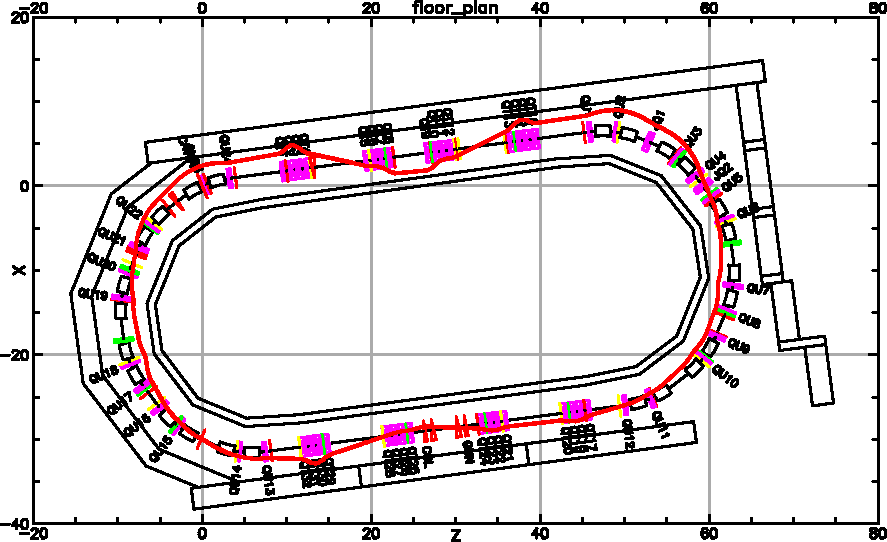
\includegraphics[width=5in]{floor-plan-orbit.pdf}
  \caption[Floor plan with orbit and building walls.]{Example Floor plan drawing with the closed orbit 
(red line) and building walls included.}
  \label{f:floor.orbit}
\end{figure}
%----------------

If element labels are to be drawn, on which side the labels are drawn can be flipped by setting 
\vn{graph%floor_plan%flip_label_side} to True.

The \vn{size_is_absolute} logical is combined with the \vn{<size>} setting for a shape to determine the
size transverse to the center line curve of the drawn shape (\sref{s:shapes}).
If \vn{size_is_absolute} is False (the default), \vn{<size>} is taken to be the size of
the shape in points (72 points is approximately 1 inch). If \vn{size_is_absolute} is True,
\vn{<size>} is taken to be the size in meters. That is, if \vn{size_is_absolute} is
False, zooming in or out will not affect the size of an element shape while if
\vn{size_is_absolute} is True, the size of an element will scale when zooming.

An overall rotation of the floor plan can be controlled by setting \vn{rotation} parameter. A
setting of 1.0 corresponds to 360$^\circ$. Positive values correspond to counter-clockwise
rotations.  Alternatively, the global coordinates at the start of the lattice can be defined in the
lattice file and this can rotate the floor plan.  Unless there is an offset specified in the lattice
file, a lattice will start at $(x, y) = (0, 0)$. Assuming that the machine lies in the horizontal
plane with no negative bends, the reference orbit will start out pointing in the negative $x$
direction and will circle clockwise in the $(x, y)$ plane.

The \vn{draw_only_first_pass} logical, if set True, suppresses drawing of \vn{multipass_slave}
lattice elements that are associated with the second and higher passes. This logical defaults to
False. Setting to True is only useful in some extreme circumstances where the plotting of additional
passes leads to large pdf/ps file sizes.

Note: If \vn{graph%ix_universe} is set to -1 the current viewed universe is used. If
\vn{graph%ix_universe} is set to -2, all universes are plotted.

Example Floor Plan template:
\begin{example}
  &tao_template_plot
    plot%name = "floor"
    plot%n_graph = 1
  /

  &tao_template_graph
    graph_index = 1
    graph%name = "1"
    graph%type = "floor_plan"
    graph%box = 1, 1, 1, 1
    graph%margin = 0.10, 0.10, 0.10, 0.10, "%BOX"
    graph%ix_universe = -2   ! Draw all universes.
    graph%x%min = -12  
    graph%x%max = 0    
    graph%x%major_div_nominal = 4
    graph%x%minor_div = 3
    graph%x%label = "SMART LABEL"
    graph%y%label = "SMART LABEL"
    graph%y%max = 2  
    graph%y%min = -1 
    graph%floor_plan%correct_distortion = T
    graph%floor_plan%size_is_absolute = T
    graph%floor_plan%view = "xz"  ! Looking from beneath
    graph%floor_plan%orbit_scale = 100
  /
\end{example}

Having \vn{graph%x%label} and \vn{graph%y%label} set to ``\vn{SMART LABEL}'' means that the actual axis labels will be 
picked appropriately based upon the setting of \vn{graph%floor_plan%view}.

To prevent the drawing of the axes set \vn{graph%draw_axes} to False.  To prevent the drawing of a
grid at the major division points set \vn{graph%draw_grid} to False.

By default, the horizontal or vertical margins of the graph will be increased so that the horizontal
scale (meters per plotting inch) is equal to the vertical scale.  If
\vn{graph%floor_plan%correct_distortion} is set to \vn{False}, this scaling will not be done.

Note: The \vn{show ele -floor} command (\sref{s:show}) can be used to view an element's global
coordinates.

%-----------------------------------------------------------------
\subsection{Defining Shapes for Lat_layout and Floor_plan Drawings}
\label{s:shapes}
\index{lat_layout drawings}
\index{floor_plan drawings}

\vn{Floor plan} (\sref{s:floor.plan}) and \vn{lattice layout} drawings use various shapes, sizes,
and colors to represent lattice elements. The association of a particular element with a given shape
is determined via two namelists: \vn{lat_layout_drawing} for the lattice layout and
\vn{floor_plan_drawing} for floor plan drawings.  Two different namelists are used since, for
example, a size that is good for a layout will not necessarily be good for a floor plan.

The file that \tao looks in to find these two namelists is set by the first file specified in the
\vn{plot_file} array set in the \vn{tao_start} namelist (\sref{s:init.global}). The default, if
\vn{plot_file} is not set, is the root initialization file.

The namelist syntax is the same for both:
\begin{example}
  &lat_layout_drawing
    include_default_shapes = <logical>
    ele_shape(N) = "<ele_id>" "<shape>" "<color>" "<size>" "<label>" <draw> 
                                                                <multi> <line_width>
  /

  &floor_plan_drawing
    ... same as lat_layout_drawing ...
  /
\end{example}
For Example:
\begin{example}
  &floor_plan_drawing
    include_default_shapes = T
    !               ele_id                  Shape        Color     Size  Label  ..etc..
    ele_shape(1) = "quadrupole::q*"         "box"        "red"     0.75  "name"  
    ele_shape(2) = "quadrupole::*"          "xbox"       "red"     0.75  "none" 
    ele_shape(3) = "sbend::sb*"             "box"        "blue"    0.37  "none"
    ele_shape(4) = "sbend::*"               "box"        "blue"    0.37  "none"  
    ele_shape(5) = "wiggler::*"             "xbox"       "green"   0.50  "name"
    ele_shape(6) = "var::quad_k1"           "circle"     "purple"  0.25  "name"
    ele_shape(7) = "data::orbit.x|design"   "vvar:box"   "orange"  0.25  "name"
    ele_shape(8) = "building_wall::*"       "solid_line" "black"    0    "none"
    ele_shape(3)%multi = T
    ele_shape(5:6)%line_width = 5, 6
  /
\end{example}
A figure is drawn for each lattice element in the lattice that matches the \vn{<ele_id>} field
(\sref{s:ele.list.format}). Thus, in the example above, \vn{ele_shape(1)} will match to all
quadrupoles whose name begins with ``q'' and \vn{ele_shape(2)} will match all quadrupoles.

Besides the usual element class prefixes (\vn{quadrupole::}, \vn{sbend::}, etc.), other prefixes
that can be used with an \vn{<ele_id>} are
\begin{example}
  data::            ! Match to \tao datum name.
  var::             ! Match to \tao variable name.
  alias::           ! Match to lattice element alias parameter.
  type::            ! Match to lattice element type parameter.
  building_wall::   ! Used in floor_plan plots.
\end{example}
The \vn{data::} prefix is used to match to data that will be used in an optimization. Thus, in the
above example, \vn{ele_shape(7)} specifies that an ``x'' will be drawn at points where there is
valid \vn{orbit.x} data. For this to work, an \vn{orbit.x} data array must be defined
(\sref{s:init.data}).

The \vn{var::} prefix is used for drawing variable locations for variables used in an
optimization. In the above example, it is assumed that a \vn{quad_k1} variable array has been
setup. A circle will be drawn at each element under control of a \vn{quad_k1} variable.

For \vn{floor_plan} drawings, the building wall (\sref{s:building.wall}) can be drawn by specifying
an \vn{ele_shape} whose name is \vn{"building_wall::<name>"} where \vn{<name>} is used to match to
the building wall section name. Use ``\vn{*}'' for \vn{<name>} to match to all names. For the
building wall, the only attribute that is relevant is the \vn{<color>} attribute.

The \vn{alias::} and \vn{type::} prefixes for \vn{<ele_id>} are used to match to the \vn{alias} and
\vn{type} string parameters of that can be set in the lattice file for each individual element.

If an element matches more than one shape,
what is drawn depends upon the setting of \vn{<multi>}. If \vn{<multi>} is False (the default) for
the first shape matched in the list of shapes, only this shape will be used.  If \vn{<multi>} is
True, \tao will draw this shape and then look for additional matches. Each time an additional match
is found, the shape is drawn and the setting of \vn{<multi>} for that shape will be used to
determine whether additional shapes are searched for. Thus \vn{<multi>} can be use to draw, for
example, a \vn{circle} shape superimposed upon a \vn{bow_tie} shape.

\tao defines a set of default shapes in case no shapes are defined in the plot file. If the
optional \vn{include_default_shapes} logical, which can be set for either \vn{floor_plan} and/or
\vn{lat_layout} shape namelists, is set to False (the default), the default shapes are not used.
If \vn{include_default_shapes} is set to True, the default shapes are appended to the list of 
shapes.

Use the \vn{show plot -floor_plan} and \vn{show plot -lat_layout} commands to see the defined
shapes. Use the \vn{set floor_plan} and \vn{set lat_layout} commands (\sref{s:set})) to set shape
parameters on the command line.

The width of a drawn shape is the width of the associated element. The exception is the \vn{"x"}
shape whose width is always the same as the height determined by the \vn{<size>} setting.

\vn{<size>} is the half height of the shape. That is, the size transverse to the longitudinal
dimension. For \vn{lat_layout} drawings, \vn{<size>} = 1.0 corresponds to full scale if the default
\vn{graph%y%min} = -1 and \vn{graph%y%max} = 1 are used. For {floor_plan} drawings, the drawn size
is also affected by the setting of \vn{graph%floor_plan%size_is_absolute} See \sref{s:floor.plan}
for more details.

The overall size of all the shapes can be scaled using the \vn{plot_page} (\sref{s:init.plot})
parameters
\begin{example}
  floor_plan_shape_scale     ! For floor_plan drawings. Default = 1
  lat_layout_shape_scale     ! For lat_layout drawings. Default = 1
\end{example}

The text size in both \vn{floor_plan} and \vn{lat_layout}
plots can be scaled by using the \vn{plot_page} parameter
\begin{example}
  legend_text_scale          ! Default = 1
\end{example}
Use the \vn{show plot} command to view these parameters. Use the
\vn{set plot_page} command to set these parameters.

\vn{<color>} is the color of the shape. Good colors to use are:
\index{element shape!color}
\begin{example}
  "black"
  "blue"
  "cyan"
  "green"
  "magenta"
  "orange"
  "purple"
  "red"
  "yellow"
\end{example}

The \vn{<line_width>} parameter is an integer that specifies the width of the lines drawn. The
default is 1.

The \vn{<label>} indicates what type of label to print next to the corresponding
element glyph. Possibilities are:
\begin{example}
  name            -- The element name (default).
  none            -- No label is drawn.
  s               -- Draw longitudinal s position.
\end{example}
The default is \vn{"name"}

The \vn{<draw>} field determines if a shape is drawn or not. The default is \vn{T}. This can be
useful for toggling on and off the drawing of shapes using the \vn{set shape} command
(\sref{s:set}).

Note: There is an old, deprecated syntax where both the lattice layout and floor plan drawings are
specified via one \vn{element_shapes} namelist.

The \vn{<shape>} parameter is the shape of the figure drawn. The \vn{<shape>} string will have the
form:
\begin{example}
  <shape-name>  or
  <prefix>:<shape-name>  
\end{example}
Valid \vn{shape-name}s are: 
\index{box}\index{xbox}
\begin{example}
  "box"            -- Rectangular box
  "bow_tie"        -- Bow-tie shape.
  "circle"         -- Circle centered at center of element.
  "diamond"        -- Diamond shape.
  <pattern_name>   -- Custom shape specified by <name>. Used with "pattern" prefix.
  "rbow_tie"       -- Bow-tie shape rotated 90 degrees.
  "d_triangle"     -- Triangle pointing ``down''.
  "l_triangle"     -- Triangle pointing ``left'' (upstream).
  "r_triangle"     -- Triangle pointing ``right'' (downstream).
  "u_triangle"     -- Triangle pointing ``up''. 
  "x"              -- "X" centered at center of element
  "xbox"           -- Rectangular box with an x through it.
  "dashed_line"    -- Only used with ele_id set to "building_wall".
  "dash_dot_line"  -- Only used with ele_id set to "building_wall".
  "dotted_line"    -- Only used with ele_id set to "building_wall".
  "solid_line"     -- Only used with ele_id set to "building_wall".
\end{example}
Valid prefixes are:
\begin{example}
  "asym_var"   -- Like "var" prefix but is not symmetric about the center line.
  "asym_vvar"  -- Like asym_var except scaled to associated variable or datum.
  "pattern"    -- Custom shape. <shape-name> here is a pattern name.
  "var"        -- Shape with variable height. 
                       The shape size is symmetric about the center line.
  "vvar"       -- Like "var" prefix except scaled to associated variable or datum.
\end{example}

For example, if an element's shape is set to \vn{var:box} or \vn{asym_var:box}, the drawn size of the
element is proportional to the element's magnetic or electric strength. The associated
\vn{<size>} setting is the multiplier used to scale from element strength to height. For
example, for a quadrupole the height is proportional to the \vn{K1} focusing strength. The
difference between \vn{var:box} or \vn{asym_var:box} is that with \vn{var:box} the drawn
box is symmetric with respect to the centerline with a size independent of the sign of the
element strength. On the other hand, with \vn{asym_var:box}, the drawn box will terminate
with one side on the centerline and the side on which it is drawn will depend upon the the
sign of the element strength. Note: Not all lattice elements can be used with a
\vn{var:box} or \vn{asym_var:box}.

A \vn{vvar:box} shape is like a \vn{var:box} and a \vn{asym_vvar:box} is like a
\vn{asym_var:box}. The difference is that \vn{vvar:box} and \vn{asym_vvar:box} shapes may only be
used when the \vn{<ele_id>} is associated with data or variables. That is, when the \vn{<ele_id>}
string starts with ``\vn{data::}'' or ``\vn{var::}''. In this case, the height of the box, instead
of being proportional to the strength of the element, is proportional to the value of the associated
datum or variable. If no datum or variable component is specified in the \vn{ele_id}, the model
value will be used. Thus, in the above example, where \vn{<ele_id>} was set to
\vn{"data::orbit.x|design"}, the design value is used.

The \vn{solid_line}, \vn{dashed_line}, \vn{dash_dot_line}, and \vn{solid_line} settings for
\vn{<shape>} is used when \vn{<ele_id>} is set to \vn{building_wall} to indicate what type of line
is to be drawn.

The \vn{pattern:<pattern_name>} shape allows for a custom pattern to be specified. Custom
patterns are specified by a \vn{shape_pattern} namelist:
\begin{example}
  &shape_pattern
    name = "<curve_name>"
    line%width = <line_width>
    pt(1) = <s>, <x>
    pt(2) = <s>, <x>
    pt(3) = ...
  /
\end{example}
Example:
\begin{example}
  &floor_plan_drawing
    ...
    ele_shape(2) = "quadrupole::*"     "pattern:q_pat"     "red"     0.75     "none" 
    ...
  /

  &shape_pattern
    name = "q_pat"
    pt(1) = 0, -1
    pt(2) = 1, -1
    pt(3) = 0.9, 1
    pt(4) = 0.1, 1
    pt(5) = 0, -1
  /
\end{example}
The \vn{name} of the \vn{shape_pattern} namelist (in this example it is "q_pat") must match the name
given by \vn{"pattern:<pattern_name>"}. The pattern is specified by a number of points. Between the
points, a line segment is drawn. In the above example, the pattern is an isosceles trapezoid.  When
drawn, the \vn{s} coordinate is scaled so that $s = 0$ corresponds to the entrance end of the
element and $s = 1$ corresponds to the exit end. The \vn{x} coordinate is scaled by the \vn{size}
attribute of the \vn{ele_shape}. The color of the line segments is set by the definition and the width
of the line segments is set by the pattern definition.

%-----------------------------------------------------------------
\subsection{Drawing Apertures}
\index{aperture drawing}
\label{s:draw.ap}

\begin{figure}
  \centering
  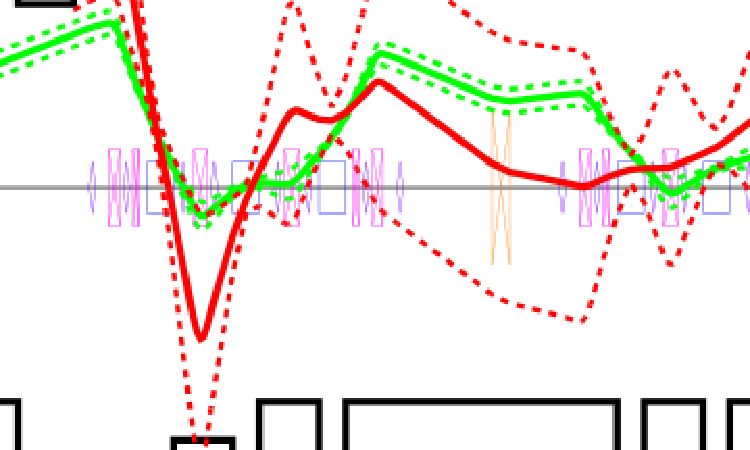
\includegraphics[width=6in]{aperture-plot.pdf}
  \caption[Example beam aperture plot.]
{Example plot of the beam aperture. In this drawing, two turns of three injected particles are drawn. The
particles start at different positions and illustrate what the size of an injected beam would be. Also drawn
(a bit faint) is a \vn{lat_layout} showing lattice element positions.}
  \label{f:aperture}
\end{figure}

Beam apertures can be defined in the \bmad lattice file. Apertures can be defined in one of three
ways. The most common is to set limit or aperture parameters for an element. Another possibility 
is to use a \vn{mask} element (which can be used to define an aperture of arbitrary shape). The
third possibility involves defining a continuous three-dimensional wall. This third possibility 
is only used with Runge-Kutta type tracking. 

To simplify things, the drawing of the beam aperture ignores any \vn{mask} elements (since the
geometry can be very complicated here) and ignores any three-dimensional walls (which are only
used for Runge-Kutta type tracking). \fig{f:aperture} shows an example of a aperture drawing.

To draw an aperture, a curve's \vn{data_source} parameter must be set to \vn{"aperture"} and the \vn{data_type} parameter is set to one of
\begin{example}
  "+x"     ! Aperture in +X direction
  "-x"     ! Aperture in -X direction
  "+y"     ! Aperture in +Y direction
  "-y"     ! Aperture in -Y direction
\end{example}
The apertures in the $+x$ and $+y$ directions will have positive values and the apertures in the
$-x$ and $-y$ directions will have negative values. Set the curve's \vn{y_axis_scale_factor} to scale
the aperture curve if needed.

The following example will graphs the horizontal orbit along with the horizontal apertures.
\begin{example}
  &tao_template_plot
    plot%name        = "x_orbit"
    plot%x_axis_type = "s"
    plot%n_graph     = 1
  /

  &tao_template_graph
    graph%name    = "x"
    graph_index   = 1

    curve(1)%data_source  = "aperture"
    curve(1)%data_type    = "+x"
    curve(1)%draw_symbols = T
    curve(1)%draw_line    = F
    curve(1)%data_source  = "aperture"
    curve(2)%data_type    = "-x"
    curve(2)%draw_symbols = T
    curve(2)%draw_line    = F
    curve(3)%data_type = "orbit.x"
  /
\end{example}
Note: Aperture curves will ignore the \vn{curve%component} parameter.

\begin{figure}
  \centering
  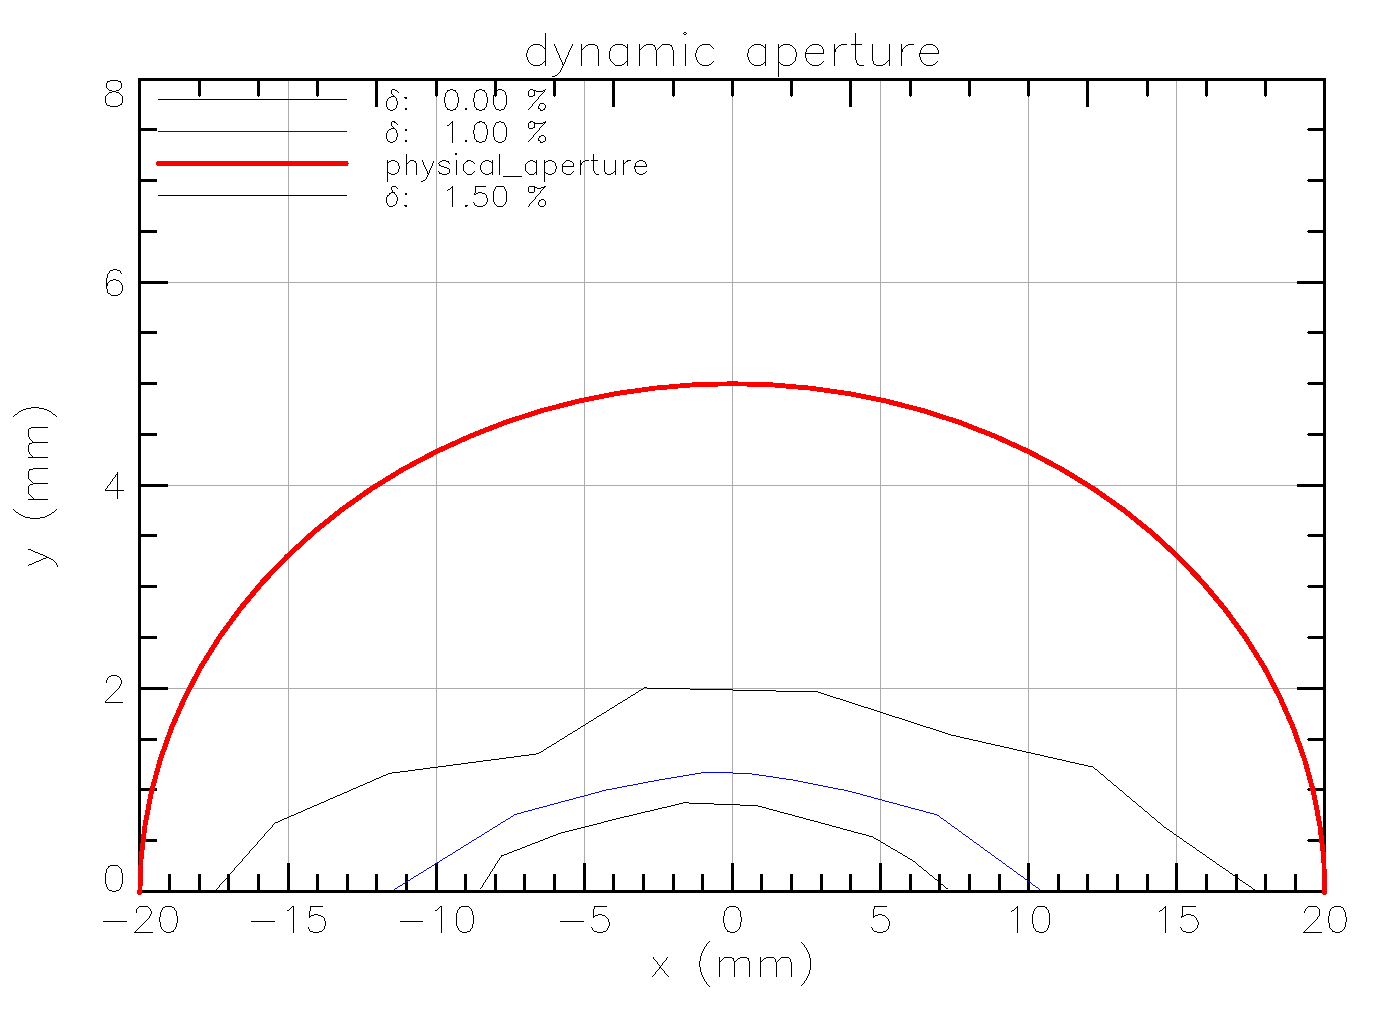
\includegraphics[width=5in]{dynamic-aperture.pdf}
  \caption{Example dynamic aperture plot.}
  \label{f:da-plot}
\end{figure}

%-----------------------------------------------------------------
\subsection{Drawing Dynamic Aperture Curves}
\index{dynamic aperture drawing}
\label{s:da.plot}

A \vn{dynamic_aperture} drawing displays the results of the dynamic aperture calculation (\sref{s:da.calc}).
Example plot setup:
\begin{example}
&tao_template_plot
  plot%name = "da"
  plot%x_axis_type = "phase_space"
  plot%n_graph = 1
/

&tao_template_graph
  graph%name = "g1"
  graph%type = "dynamic_aperture"
  graph_index = 1
  graph%x%label = "x (mm)"
  graph%x_axis_scale_factor = 1000  ! Plot in mm.
  graph%y%label = "y (mm)"
  curve(1)%line%color = "red"
  curve(1)%data_type = 'beam_ellipse'
  curve(1)%line%width = 5
  curve(1)%legend_text = '10 sigma beam ellipse'
  curve(1)%draw_symbols = F
  curve(1:10)%y_axis_scale_factor = 10*1000  ! Plot in mm.
  curve(2:10)%draw_symbols = 9*T
  curve(2:10)%data_type = 9*"dynamic_aperture"
  curve(2:10)%data_index = 1, 2, 3, 4, 5, 6, 7, 8, 9
  curve(3)%symbol%color = "purple"
  curve(3)%line%color = "purple"
/
\end{example}
This will produce a plot similar to Fig.~\ref{f:da-plot}.  Each curve represents a dynamic aperture
scan at fixed initial momentum $p_z$.

Dynamic aperture curves can have the following \vn{%data_type} parameters:
\begin{example}
  "dynamic_aperture"        ! Curve points are with respect to the closed orbit (x,y).
  "dynamic_aperture_ref0"   ! Curve points are with respect to x = y = 0.
  "beam_ellipse"            ! Draws the beam ellipse within the [min_angle, max_angle] range.
  "beam_ellipse_full"       ! Draws the entire beam ellipse.
\end{example}

In the above example, the first curve has \vn{%data_type} set to \vn{"beam_ellipse"}. This results
in the half ellipse in red since the [min_angle, max_angle] set in the \vn{tao_dynamic_aperture}
namelist for this example was [0, pi]. If the entire ellipse is desired to be drawn, the
\vn{%data_type} can be set to \vn{"beam_ellipse_full"}. The scale of the ellipse drawn is set by the
\vn{ellipse_scale} parameter of the \vn{tao_dynamic_aperture} namelist (\sref{s:da.calc}). The default value is
10 so that a $10 \, \sigma$ ellipse will be drawn by default. Also used in calculating the ellipse
curve are the settings of \vn{a_emit} and \vn{b_emit} emittances also set in the same namelist.

There are 10 curves defined in the example. Curves 2 through 10 have \vn{%data_type} set to
\vn{"dynamic_aperture"}. Each curve here represents one dynamic aperture scan. The scan index is set
by a curve's \vn{%data_index} parameter. An index of "1" denotes the first scan with the initial
momentum set by the first value in the \vn{pz} array set in the \vn{tao_dynamic_aperture} namelist
(\sref{s:da.calc}). If a curve has an index that is greater than the number of scans, that curve is ignored.

%-----------------------------------------------------------------
\subsection{Drawing a Histogram}
\index{histogram drawing}
\label{s:histogram}

A \vn{histogram} drawing displays a histogram of phase space beam density. Histogram plotting is
associated with a \vn{graph} by setting \vn{graph%type} equal to \vn{"histogram"}. The concepts here
are similar to \vn{phase space} plotting (\sref{s:phase.space}). An example is shown in
Fig.~\ref{f:histogram}, using the example histogram template:
\begin{example}
&tao_template_plot
  plot%name = "zhist"
  plot%n_graph = 1
/

&tao_template_graph
  graph_index = 1
  graph%name = "z"
  graph%type = "histogram"
  graph%box = 1, 1, 1, 1
  graph%title = "Bunch Histogram: Z"
  graph%margin =  0.15, 0.06, 0.12, 0.12, "%BOX"
  graph%x%min = -6
  graph%x%max =  6
  graph%x%label = "z (mm)"
  graph%y%label = "Current (A)"
  graph%y%label_offset = .1
  graph%x_axis_scale_factor = 1000.00 !m->mm

  curve(1)%hist%density_normalized = T
  curve(1)%hist%weight_by_charge = T
  curve(1)%hist%number = 100
  curve(1)%line%color = "blue"
  curve(1)%line%pattern = "dashed"
  curve(1)%y_axis_scale_factor = 299792458  !Q/m * c_light
  curve(1)%data_type = "z" 
  curve(1)%data_source = "beam_tracking"
  curve(1)%ele_ref_name = "BEGINNING"
  curve(1)%symbol%type = "dot"
/
\end{example}

\begin{figure}
  \centering
  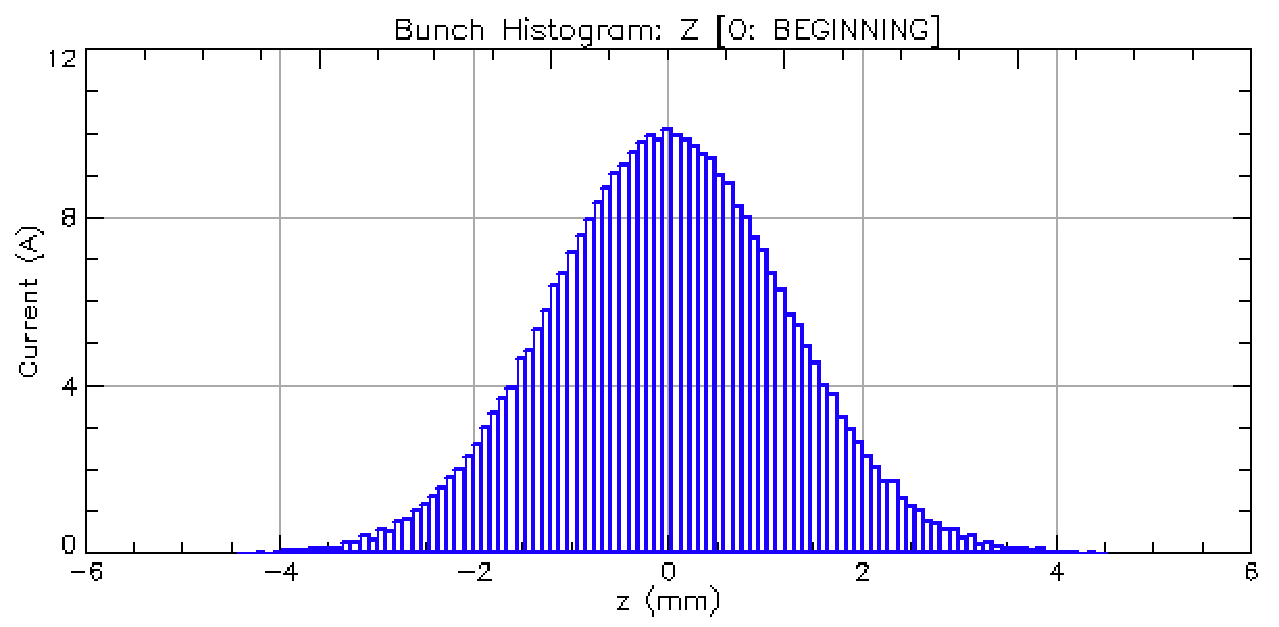
\includegraphics[width=5in]{histogram.pdf}
  \caption{Example histogram plot.}
  \label{f:histogram}
\end{figure}

For a \vn{"histogram"} type graph, \vn{curve%data_type} determines what coordinate is plotted along
the x-axis.  Valid \vn{curve%data_type} values are:
\index{x}\index{px}\index{y}\index{py}\index{z}\index{pz}
\begin{example}
  "x"
  "px"
  "y"
  "py"
  "z"
  "pz"
  "intensity"       -- Photon total intensity 
  "intensity_x"     -- Photon intensity along x-axis 
  "intensity_y"     -- Photon intensity along y-axis
  "phase_x"         -- Photon phase along x-axis
  "phase_y"         -- Photon phase along y-axis
\end{example}
In this example above, the $x$-axis of the plot will correspond to the $z$ phase space coordinate.

The maximum and minimum of the bins is set automatically to fit the data.  The
\vn{curve%hist%number} establishes the number of bins. Alternatively, if \vn{curve%hist%number = 0},
then \vn{curve%hist%width} establishes the width of the histogram bins and sets the number
automatically.

If \vn{curve%hist%density_normalized = T}, then the height of a bin will be divided by its width. If
\vn{curve%hist%weight_by_charge = T}, then the particle charge will be used to bin, otherwise the
particle count will be used to bin.

The \vn{curve%hist%center} will insure that a bin will be centered at this location.

\index{curve!ele_ref_name}
To change the place in the lattice where the data for the \vn{histogram} is evaluated, use the
\vn{set curve ele_ref_name} command.

If \vn{graph%type} is \vn{"histogram"} then \vn{curve%data_source} 
must be either:
\begin{example}
  "beam"
  "multi_turn_orbit"
  "rel_multi_turn_orbit"
\end{example} 
\vn{"beam"} indicates that the points of the histogram plot will be obtained correspond to the
positions of the particles within a tracked beam. 

Setting \vn{curve%data_source} to \vn{"multi_turn_orbit"} or \vn{"rel_multi_turn_orbit"} is used for
rings where a single particle is tracked multiple turns and the position of this particle is
recorded each turn. The number of turns is determined by the setting of \vn{curve%n_turn}. The
starting position for the tracking is set by setting the \vn{particle_start[x]},
\vn{particle_start[px]}, etc.  parameters in the lattice file (see the \bmad manual for
details). The difference between \vn{"multi_turn_orbit"} and \vn{"rel_multi_turn_orbit"} is that
\vn{"rel_multi_turn_orbit"} is drawn relative to the phase space point
\begin{equation}
  p_{z0} \cdot (\eta_x, \eta'_x, \eta_y, eta'_y, 0, 0)
\end{equation}
where $p_{z0}$ is the value of the particle's initial $p_z$ and $\eta$ is the dispersion at the
reference element where the orbit is being evaluated for the plot.

%%-----------------------------------------------------------------
%\subsection{Drawing the Beam Chamber Wall}
%\index{beam chamber wall}
%\label{s:beam.wall.draw}
%
%If a beam chamber wall has been defined in the lattice file, This wall can be drawn in a \vn{curve}
%by setting \vn{curve%type} to \vn{"beam_chamber_wall"}.
%
%Beam chamber walls are drawn, like a \vn{lat_layout}, on a one dimensional line as a function of
%longitudinal position along the machine centerline.
%
%Note: Use the command \vn{show ele -wall} to print information about the beam chamber wall for a
%particular element.

%%-----------------------------------------------------------------
%\subsection{Drawing Controller Element Curves}
%\index{drawing controller element curves}
%\label{s:draw.control}
%
%A controller element is a \bmad lattice element that controls the parameters of other elements.
%There are three types of controller elements: \vn{groups}, \vn{overlays}, and \vn{rampers}. See 
%the Bmad manual for more details. A controller has one or more independent variables that control
%parameters of other elements. The response of a controlled parameter as a function of any one of 
%controller variables may be plotted.

%% Put under graph%type:
%%  "control_curve"      ! Plot slave response for a controller lattice element (\sref{s:draw.control})


%-----------------------------------------------------------------
\subsection{Drawing a Key Table}
\index{key table}
\label{s:key.table}

A \vn{key table} displays information about variables bound to keyboard keys \sref{s:key.bind}. Key
bindings are used in \vn{single mode}. An example is shown in Figure~\ref{f:layout.table}. A
template to create a key table looks like:
\begin{example}
  &tao_template_plot
    plot%name = "table" 
    plot%n_graph = 1
  /

  &tao_template_graph
    graph%type = "key_table" 
    graph_index = 1
  /
\end{example}

The number in the upper left corner, to the left of the first column, (\vn{1} in
Fig.~\ref{f:layout.table}) shows the active \vn{key bank}. The columns in the Key Table are:
\begin{example}
  Ix         ! Key index.
  Name       ! Element name whose attribute is bound.
  Attrib     ! Name of the element attribute that is bound.
  Value      ! Current value of bound attribute.
  Value0     ! Initial value of bound attribute.
  Delta      ! Change in value when the appropriate key is pressed.
  Uni        ! Universe that contains the element.
  Opt        ! Shows if bound attribute is used in an optimization.
\end{example}

Note that in a \vn{Lattice Layout}, if a displayed element has a bound attribute, then the key index
number will be displayed just above the element's glyph.

The \vn{key_table} is drawn with respect to the upper left hand corner of the region in which it is
placed.

%-----------------------------------------------------------------
\subsection{Phase Space Plotting}
\index{phase space plotting}
\label{s:phase.space}

\begin{figure}
  \centering
  \begin{subfigure}[b]{0.45\textwidth}
    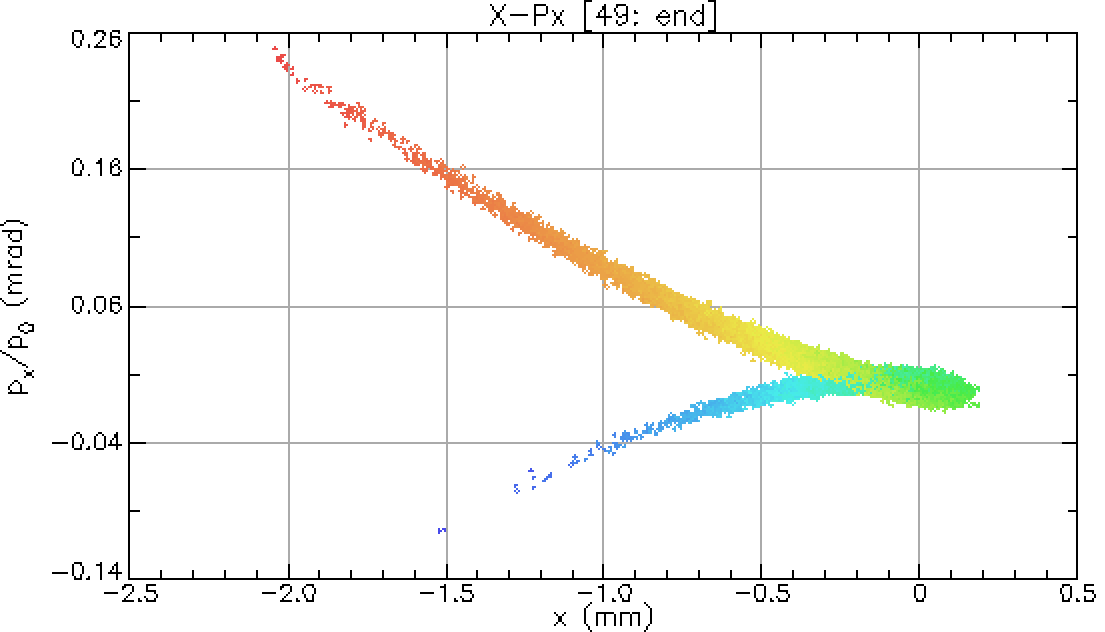
\includegraphics[width=\textwidth]{plot-color-xpx}
    \caption{Horizontal phase space}
  \end{subfigure}
  \begin{subfigure}[b]{0.45\textwidth}
    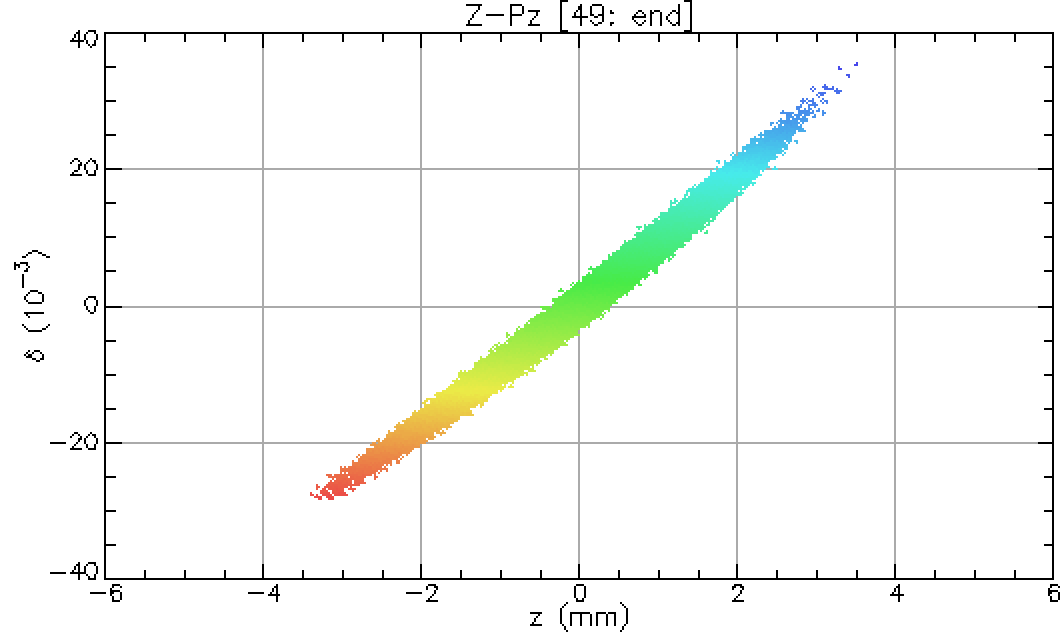
\includegraphics[width=\textwidth]{plot-color-zpz}
    \caption{Longitudinal phase space}
  \end{subfigure}  
  \caption{Example Phase Space plot, with points colored by the \vn{pz} coordinate.}
  \label{f:phase.space}
\end{figure}

A \vn{phase space} plot displays a particle or particles phase space coordinates at a given
location. Phase space plotting is associated with a \vn{graph} by setting \vn{graph%type} equal to
\vn{"phase_space"}. The concepts here are similar to \vn{data} plotting (\sref{s:graph.types}). An
example is show in Figure~\ref{f:phase.space}.  Example Phase Space template:
\begin{example}
&tao_template_plot
  plot%name = "xphase"
  plot%n_graph = 1
/

&tao_template_graph
  graph_index = 1
  graph%name = "x"
  graph%type = "phase_space"
  graph%box = 1, 1, 1, 1
  graph%title = "X-Px"
  graph%margin =  0.15, 0.06, 0.12, 0.12, "%BOX"
  graph%x%min =   -2.5
  graph%x%max = 0.5
  graph%x%label = "x (mm)"
  graph%x_axis_scale_factor = 1000.00 !m->mm
  graph%y%label =  "p\textbackslash{}dx\textbackslash{}u/p\textbackslash{}d0\textbackslash{}u (mrad)"
  graph%y%major_div = 4
  graph%y%label_offset=.4
  curve(1)%data_type_x = "x" 
  curve(1)%data_type   = "px" 
  curve(1)%y_axis_scale_factor = 1000 !rad->mrad
  curve(1)%data_source = "beam_tracking"
  curve(1)%ele_ref_name = "END"
  curve(1)%symbol%type = 1
  curve(1)%z_color%data_type = "pz"
  curve(1)%z_color%is_on = T
  /
\end{example}

For a \vn{"phase_space"} type graph, \vn{curve%data_type_x} determines what phase space coordinate
is plotted along the x-axis and \vn{curve%data_type} determines what phase space coordinate is
plotted along the y-axis. Phase space coordinates are one of:
\index{x}\index{px}\index{y}\index{py}\index{z}\index{pz}
\begin{example}
  "x",  "px",  "y",  "py",  "z",  "pz",
  "intensity",  "intensity_x",  "intensity_y"     ! Photon intensity
  "phase_x", "phase_y"                            ! Photon coherent phase
\end{example}
In this example above, the $x$-axis of the plot will correspond to the $z$ phase space coordinate
and the $pz$-axis will correspond to the $px$ coordinate.

\index{curve!ele_ref_name}
To change the place in the lattice where the data for the \vn{phase_space} curve is evaluated, use
the \vn{set curve ele_ref_name} command.

Points can be colored by another phase space coordinate by activating \vn{z_color%is_on = T}.  The
available curve options and defaults for \vn{curve(N)%z_color} components are:
\begin{example}
  %is_on = F
  %data_type = "" 
  %min = 0
  %max = 0
  %autoscale = T
\end{example}
These can be the init file, or in Tao using the \vn{set curve} command.  The \vn{%data_type} can be
set to any of the available phase space coordinates.  \vn{%min} and \vn{%max} specify the
minimum and maximum of this coordinate to be used in the color range. Values above or below this
range will be colored Black or Grey, respectively.  If \vn{%autoscale} = True, then these will be
set automatically based on the limits of the \vn{%data_type} coordinate.

If \vn{graph%type} is \vn{"phase_space"} then \vn{curve%data_source} 
must be either:
\begin{example}
  "beam"
  "multi_turn_orbit"
  "twiss"
\end{example} 
\vn{"beam"} indicates that the points of the phase space plot will be obtained correspond to the
positions of the particles within a tracked beam. \vn{multi_turn_orbit"} is used for rings where a
single particle is tracked multiple turns and the position of this particle is recorded each
turn. In this case, a \vn{d2_data} structure must have been set up to hold the turn--by--turn
orbit. This \vn{d2_data} structure must be called \vn{multi_turn_orbit} and must have \vn{d1_data}
data arrays for the phase space planes to be plotted. For example, if the phase space plot is \vn{x}
versus \vn{px}, then there must be \vn{d1_data} arrays named \vn{"x"} and \vn{"px"}. The number of
turns is determined by the setting of \vn{ix_max_data} in the \vn{tao_d1_data} namelist
(\sref{s:init.data}). Using \vn{"twiss"} as the \vn{curve%data_source} indicates that the phase
space plot will be an ellipse whose shape is based upon the Twiss and coupling parameters, and the
normal mode emittances. If the normal mode emittances have not been computed then a nominal value of
1~$\mu$m-rad is used.
